% Problems, Chapter 15: Legendre Functions
% Arfken, Weber & Harris, Mathematical Methods for Physicists, 7th ed.
% Requires: amsmath, amssymb, tikz

\section*{Problems}

\Needspace{8\baselineskip}
\subsection*{15.1 Legendre Polynomials}

\Needspace{5\baselineskip}
\par\bigskip
\noindent\textbf{15.1.1}\quad Derive the Legendre ODE by manipulation
of the Legendre polynomial recurrence relations. Suggested starting
point: Eqs.~(15.24) and (15.25).
\solution
The two needed recurrences, Eqs.~(15.24) and (15.25), are
\[
P'_{n-1}=-nP_n+xP'_n,\qquad
(1-x^2)P'_n=nP_{n-1}-nxP_n.
\]
Differentiate the second, including both product derivatives:
\[
(1-x^2)P_n''-2xP_n'
=nP'_{n-1}-nP_n-nxP_n'.
\]
Insert $n$ times the first recurrence for $nP'_{n-1}$ on the right; the
terms $\pm nxP_n'$ cancel:
\[
n(-nP_n+xP_n')-nP_n-nxP_n'=-n^2P_n-nP_n=-n(n+1)P_n.
\]
Moving this term to the left gives
\[
\boxed{(1-x^2)P_n''-2xP_n'+n(n+1)P_n=0}.
\]
For $n=0$, $P_0=1$ verifies the equation directly, so no undefined
$P_{-1}$ is needed at that endpoint.

\Needspace{5\baselineskip}
\par\bigskip
\noindent\textbf{15.1.2}\quad Derive the following closed formula for
the Legendre polynomials $P_{n}(x)$,
\[
P_{n}(x)=\sum_{k=0}^{[n/2]}(-1)^{k}
\frac{(2n-2k)!}{2^{n}k!(n-k)!(n-2k)!}\,x^{n-2k},
\]
where $[n/2]$ stands for the integer part of $n/2$.
\par\emph{Hint.}~Further expand Eq.~(15.12) and rearrange the
resulting double sum.
\solution
Start in a sufficiently small disk about $t=0$, where the binomial
series converges:
\[
(1-2xt+t^2)^{-1/2}
=\sum_{j=0}^\infty\binom{-1/2}{j}(-2xt+t^2)^j.
\]
Expand each power by the binomial theorem,
$(t^2-2xt)^j=\sum_{k=0}^j\binom jk(t^2)^k(-2xt)^{j-k}$: choosing $k$
copies of $t^2$ from the $j$ factors, the other $j-k$ copies contribute
$(-2xt)^{j-k}$, so the resulting term is
\[
\binom{-1/2}{j}\binom jk(-2x)^{j-k}t^{j+k}.
\]
For $2|xt|+|t|^2<1$ this double series converges absolutely (with every
term replaced by its absolute value it sums to $(1-2|xt|-|t|^2)^{-1/2}$),
so its terms may be collected by powers of $t$.
To obtain $t^n$, set $j=n-k$. The condition $0\le k\le j$
becomes $2k\le n$, i.e., $0\le k\le\lfloor n/2\rfloor$. Therefore
\[
P_n(x)=\sum_{k=0}^{\lfloor n/2\rfloor}
\binom{-1/2}{n-k}\binom{n-k}{k}(-2x)^{n-2k}.
\]
Use
\[
\binom{-1/2}{j}=\frac{(-\frac12)(-\frac32)\cdots(-\frac{2j-1}2)}{j!}
=(-1)^j\frac{(2j-1)!!}{2^jj!}=(-1)^j\frac{(2j)!}{2^{2j}(j!)^2}
\]
(since $(2j-1)!!=(2j)!/(2^jj!)$) with $j=n-k$, together with
$\binom{n-k}{k}=(n-k)!/[k!(n-2k)!]$.
The sign becomes $(-1)^{n-k+n-2k}=(-1)^k$ and the power of two is
$2^{n-2k-2(n-k)}=2^{-n}$. The remaining factorials combine as
\[
\frac{(2n-2k)!}{[(n-k)!]^2}\,\frac{(n-k)!}{k!(n-2k)!}
=\frac{(2n-2k)!}{k!(n-k)!(n-2k)!},
\]
so that
\[
\boxed{P_n(x)=\sum_{k=0}^{\lfloor n/2\rfloor}
(-1)^k\frac{(2n-2k)!}{2^nk!(n-k)!(n-2k)!}x^{n-2k}}.
\]
Although the generating series was used locally in $t$, the coefficient
is a polynomial identity and holds for every finite complex $x$.

\Needspace{5\baselineskip}
\par\bigskip
\noindent\textbf{15.1.3}\quad By differentiation and direct
substitution of the series form given in Exercise~15.1.2, show that
$P_{n}(x)$ satisfies the Legendre ODE. Note that there is no
restriction on $x$. We may have any $x$, $-\infty<x<\infty$, and
indeed any $z$ in the entire finite complex plane.
\solution
Write $P_n=\sum_{k=0}^{\lfloor n/2\rfloor}A_kx^{n-2k}$, with
$A_k=(-1)^k(2n-2k)!/[2^nk!(n-k)!(n-2k)!]$
as in Exercise 15.1.2. With $D=d/dx$, the Legendre operator
$L_n=(1-x^2)D^2-2xD+n(n+1)$ acts on a monomial as
\[
L_n[x^j]=(1-x^2)j(j-1)x^{j-2}-2jx^j+n(n+1)x^j
=j(j-1)x^{j-2}+[n(n+1)-j(j+1)]x^j,
\]
since $-j(j-1)-2j=-j(j+1)$.
For $1\le k\le\lfloor n/2\rfloor$, the power $x^{n-2k}$ in $L_n[P_n]$
receives the second term of $L_n[A_kx^{n-2k}]$ and the first term of
$L_n[A_{k-1}x^{n-2k+2}]$ (with $j=n-2k+2$). Its total coefficient is
\[
(n-2k+2)(n-2k+1)A_{k-1}
+2k(2n-2k+1)A_k,
\]
because
$n(n+1)-(n-2k)(n-2k+1)=4kn-4k^2+2k=2k(2n-2k+1)$.
The ratio of consecutive coefficients is
\begin{align*}
\frac{A_k}{A_{k-1}}
&=-\frac{(2n-2k)!}{(2n-2k+2)!}\,\frac{(k-1)!}{k!}\,
\frac{(n-k+1)!}{(n-k)!}\,\frac{(n-2k+2)!}{(n-2k)!}\\
&=-\frac{(n-k+1)(n-2k+2)(n-2k+1)}{k(2n-2k+2)(2n-2k+1)}
=-\frac{(n-2k+2)(n-2k+1)}{2k(2n-2k+1)},
\end{align*}
where the last step uses $2n-2k+2=2(n-k+1)$.
Thus every displayed coefficient is zero. The leading coefficient
($k=0$) is multiplied by $n(n+1)-n(n+1)=0$.
At the bottom, the last monomial is either $1$ or $x$, whose second
derivative is zero, so no lower power remains. Hence $L_n[P_n]=0$
identically. All manipulations concern finite polynomials, which proves
the claim on the entire finite complex plane.

\Needspace{5\baselineskip}
\par\bigskip
\noindent\textbf{15.1.4}\quad The shifted Legendre polynomials,
designated by the symbol $P_{n}^{*}(x)$ (where the asterisk does not
mean complex conjugate) are orthogonal with unit weight on $[0,1]$,
with normalization integral
$\langle P_{n}^{*}|P_{n}^{*}\rangle=1/(2n+1)$. The $P_{n}^{*}$ through
$n=6$ are shown in Table~15.2.
\begin{center}
\begin{tabular}{l}
\multicolumn{1}{c}{Table 15.2\quad Shifted Legendre Polynomials}\\[4pt]
\toprule
$P_{0}^{*}(x)=1$\\
$P_{1}^{*}(x)=2x-1$\\
$P_{2}^{*}(x)=6x^{2}-6x+1$\\
$P_{3}^{*}(x)=20x^{3}-30x^{2}+12x-1$\\
$P_{4}^{*}(x)=70x^{4}-140x^{3}+90x^{2}-20x+1$\\
$P_{5}^{*}(x)=252x^{5}-630x^{4}+560x^{3}-210x^{2}+30x-1$\\
$P_{6}^{*}(x)=924x^{6}-2772x^{5}+3150x^{4}-1680x^{3}+420x^{2}-42x+1$\\
\bottomrule
\end{tabular}
\end{center}
\begin{enumerate}
\item[(a)] Find the recurrence relation satisfied by the $P_{n}^{*}$.
\item[(b)] Show that all the coefficients of the $P_{n}^{*}$ are
integers.
\end{enumerate}
\par\emph{Hint.}~Look at the closed formula in Exercise~15.1.2.
\solution
The listed normalization and signs are obtained by
$P_n^*(x)=P_n(2x-1)$. Indeed, $y=2x-1$ (so $dx=dy/2$, and $x=0,1$
become $y=-1,1$) gives
\[
\int_0^1P_n^*P_m^*dx
=\frac12\int_{-1}^1P_n(y)P_m(y)dy
=\frac12\,\frac{2\delta_{nm}}{2n+1}
=\frac{\delta_{nm}}{2n+1}.
\]
\erratum{The Instructor's Manual's last expression on p.~232 retains an
extra factor $1/2$. The change of variable contributes $1/2$, but the
unshifted norm contributes $2/(2n+1)$, leaving $1/(2n+1)$ as stated
correctly in the textbook.}
(a) Replace the argument in
$(n+1)P_{n+1}(y)=(2n+1)yP_n(y)-nP_{n-1}(y)$ by $y=2x-1$:
\[
\boxed{(n+1)P_{n+1}^*(x)
=(2n+1)(2x-1)P_n^*(x)-nP_{n-1}^*(x)}.
\]
The initial polynomials are $P_0^*=1$, $P_1^*=2x-1$. For example,
$n=1$ gives $2P_2^*=3(2x-1)^2-1=12x^2-12x+2$, i.e.,
$P_2^*=6x^2-6x+1$, as in the table.

(b) The recurrence alone involves division by $n+1$, so an explicit
coefficient formula is more useful for proving integrality.
Transform Rodrigues's formula
$P_n(y)=D_y^n(y^2-1)^n/(2^nn!)$, where $D_y=d/dy$, using
$D_y=\tfrac12D_x$ (with $D_x=d/dx$, since $dy=2\,dx$) and
$y^2-1=4x^2-4x=4x(x-1)$:
\[
P_n^*(x)=\frac1{2^nn!}\,\frac1{2^n}D_x^n[4^nx^n(x-1)^n]
=\frac1{n!}D_x^n[x^n(x-1)^n].
\]
Expand $(x-1)^n=\sum_{k=0}^n(-1)^{n-k}\binom nk x^k$, so that
$x^n(x-1)^n=\sum_{k=0}^n(-1)^{n-k}\binom nk x^{n+k}$, and differentiate
with $D_x^nx^{n+k}=\frac{(n+k)!}{k!}x^k$:
\[
P_n^*(x)=\sum_{k=0}^n(-1)^{n-k}
\binom nk\frac{(n+k)!}{n!k!}x^k
=\boxed{\sum_{k=0}^n(-1)^{n-k}\binom nk\binom{n+k}{k}x^k}.
\]
Every coefficient is a signed product of integers.

\Needspace{5\baselineskip}
\par\bigskip
\noindent\textbf{15.1.5}\quad Given the series
\[
\alpha_{0}+\alpha_{2}\cos^{2}\theta+\alpha_{4}\cos^{4}\theta
+\alpha_{6}\cos^{6}\theta=a_{0}P_{0}+a_{2}P_{2}+a_{4}P_{4}+a_{6}P_{6},
\]
where the arguments of the $P_{n}$ are $\cos\theta$, express the
coefficients $\alpha_{i}$ as a column vector $\boldsymbol{\alpha}$ and
the coefficients $a_{i}$ as a column vector $\mathbf{a}$ and determine
the matrices $\mathsf{A}$ and $\mathsf{B}$ such that
\[
\mathsf{A}\boldsymbol{\alpha}=\mathbf{a}
\quad\text{and}\quad\mathsf{B}\mathbf{a}=\boldsymbol{\alpha}.
\]
Check your computation by showing that $\mathsf{AB}=\mathbf{1}$ (unit
matrix). Repeat for the odd case
\[
\alpha_{1}\cos\theta+\alpha_{3}\cos^{3}\theta+\alpha_{5}\cos^{5}\theta
+\alpha_{7}\cos^{7}\theta=a_{1}P_{1}+a_{3}P_{3}+a_{5}P_{5}+a_{7}P_{7}.
\]
\par\emph{Note.}~$P_{n}(\cos\theta)$ and $\cos^{n}\theta$ are
tabulated in terms of each other in AMS-55 (see Additional Readings
for the complete reference).
\solution
Put $x=\cos\theta$ and order the even columns as
$\boldsymbol\alpha=(\alpha_0,\alpha_2,\alpha_4,\alpha_6)^T$,
$\mathbf a=(a_0,a_2,a_4,a_6)^T$. The coefficients of
$P_0,P_2,P_4,P_6$ in ascending powers of $x$ give the columns of
$\mathsf B_e$:
\[
\boxed{\mathsf B_e=
\begin{pmatrix}
1&-1/2&3/8&-5/16\\
0&3/2&-15/4&105/16\\
0&0&35/8&-315/16\\
0&0&0&231/16
\end{pmatrix}}.
\]
The rows of $\boldsymbol\alpha=\mathsf B_e\mathbf a$ read
\begin{align*}
\alpha_6&=\tfrac{231}{16}a_6,\qquad
\alpha_4=\tfrac{35}8a_4-\tfrac{315}{16}a_6,\\
\alpha_2&=\tfrac32a_2-\tfrac{15}4a_4+\tfrac{105}{16}a_6,\qquad
\alpha_0=a_0-\tfrac12a_2+\tfrac38a_4-\tfrac5{16}a_6.
\end{align*}
Solve them from the last one upward, inserting each result in the next:
\begin{align*}
a_6&=\tfrac{16}{231}\alpha_6,\\
a_4&=\tfrac8{35}\bigl(\alpha_4+\tfrac{315}{16}a_6\bigr)
=\tfrac8{35}\alpha_4+\tfrac{24}{77}\alpha_6,\\
a_2&=\tfrac23\bigl(\alpha_2+\tfrac{15}4a_4-\tfrac{105}{16}a_6\bigr)
=\tfrac23\bigl(\alpha_2+\tfrac67\alpha_4+\tfrac57\alpha_6\bigr)
=\tfrac23\alpha_2+\tfrac47\alpha_4+\tfrac{10}{21}\alpha_6,\\
a_0&=\alpha_0+\tfrac12a_2-\tfrac38a_4+\tfrac5{16}a_6
=\alpha_0+\tfrac13\alpha_2+\tfrac15\alpha_4+\tfrac17\alpha_6.
\end{align*}
Inside the parentheses of $a_2$, the coefficient of $\alpha_6$ is
$\frac{15}4\cdot\frac{24}{77}-\frac{105}{16}\cdot\frac{16}{231}
=\frac{90}{77}-\frac{35}{77}=\frac57$; in $a_0$, those of $\alpha_4$ and
$\alpha_6$ are $\frac27-\frac3{35}=\frac15$ and
$\frac5{21}-\frac9{77}+\frac5{231}=\frac{33}{231}=\frac17$.
Thus
\[
\boxed{\mathsf A_e=
\begin{pmatrix}
1&1/3&1/5&1/7\\
0&2/3&4/7&10/21\\
0&0&8/35&24/77\\
0&0&0&16/231
\end{pmatrix}}.
\]
Read by columns, $\mathsf A_e$ gives the Legendre expansions
$x^2=\frac13P_0+\frac23P_2$, $x^4=\frac15P_0+\frac47P_2+\frac8{35}P_4$,
and $x^6=\frac17P_0+\frac{10}{21}P_2+\frac{24}{77}P_4+\frac{16}{231}P_6$.
The diagonal entries of $\mathsf A_e\mathsf B_e$ are products of
diagonal entries, $1\cdot1$, $\frac23\cdot\frac32$,
$\frac8{35}\cdot\frac{35}8$, $\frac{16}{231}\cdot\frac{231}{16}$, all
equal to one. The six upper off-diagonal entries (row $i$ of
$\mathsf A_e$ times column $j$ of $\mathsf B_e$, $i<j$, in the order
$(1,2),(1,3),(1,4)$ and $(2,3),(2,4),(3,4)$) are, explicitly,
\[
-\tfrac12+\tfrac12,\quad
\tfrac38-\tfrac54+\tfrac78,\quad
-\tfrac5{16}+\tfrac{35}{16}-\tfrac{63}{16}+\tfrac{33}{16},
\]
\[
-\tfrac52+\tfrac52,\quad
\tfrac{35}{8}-\tfrac{45}{4}+\tfrac{55}{8},\quad
-\tfrac92+\tfrac92.
\]
All vanish, and entries below the diagonal vanish by triangularity.
Hence $\mathsf A_e\mathsf B_e=\mathsf1$.

For the odd case use the order $1,3,5,7$. The coefficients of
$P_1,P_3,P_5,P_7$ give the columns of $\mathsf B_o$ below, and the same
back substitution, from
$\alpha_7=\frac{429}{16}a_7$,
$\alpha_5=\frac{63}8a_5-\frac{693}{16}a_7$,
$\alpha_3=\frac52a_3-\frac{35}4a_5+\frac{315}{16}a_7$,
$\alpha_1=a_1-\frac32a_3+\frac{15}8a_5-\frac{35}{16}a_7$, gives
\begin{align*}
a_7&=\tfrac{16}{429}\alpha_7,\qquad
a_5=\tfrac8{63}\bigl(\alpha_5+\tfrac{693}{16}a_7\bigr)
=\tfrac8{63}\alpha_5+\tfrac8{39}\alpha_7,\\
a_3&=\tfrac25\bigl(\alpha_3+\tfrac{35}4a_5-\tfrac{315}{16}a_7\bigr)
=\tfrac25\bigl(\alpha_3+\tfrac{10}9\alpha_5+\tfrac{35}{33}\alpha_7\bigr)
=\tfrac25\alpha_3+\tfrac49\alpha_5+\tfrac{14}{33}\alpha_7,\\
a_1&=\alpha_1+\tfrac32a_3-\tfrac{15}8a_5+\tfrac{35}{16}a_7
=\alpha_1+\tfrac35\alpha_3+\tfrac37\alpha_5+\tfrac13\alpha_7.
\end{align*}
Inside the parentheses of $a_3$, the coefficient of $\alpha_7$ is
$\frac{35}4\cdot\frac8{39}-\frac{315}{16}\cdot\frac{16}{429}
=\frac{770-315}{429}=\frac{35}{33}$, and in $a_1$ the coefficients of
$\alpha_5$ and $\alpha_7$ are $\frac23-\frac5{21}=\frac37$ and
$\frac7{11}-\frac5{13}+\frac{35}{429}=\frac{143}{429}=\frac13$.
Therefore
\[
\boxed{\mathsf B_o=
\begin{pmatrix}
1&-3/2&15/8&-35/16\\
0&5/2&-35/4&315/16\\
0&0&63/8&-693/16\\
0&0&0&429/16
\end{pmatrix}},\qquad
\boxed{\mathsf A_o=
\begin{pmatrix}
1&3/5&3/7&1/3\\
0&2/5&4/9&14/33\\
0&0&8/63&8/39\\
0&0&0&16/429
\end{pmatrix}}.
\]
In the same order as for the even case, the six upper off-diagonal
entries of $\mathsf A_o\mathsf B_o$ are
\[
-\tfrac32+\tfrac32,\quad
\tfrac{15}8-\tfrac{21}4+\tfrac{27}8,\quad
-\tfrac{35}{16}+\tfrac{189}{16}-\tfrac{297}{16}+\tfrac{143}{16},
\]
\[
-\tfrac72+\tfrac72,\quad
\tfrac{63}8-\tfrac{77}4+\tfrac{91}8,\quad
-\tfrac{11}2+\tfrac{11}2,
\]
again zero, with diagonal entries $1\cdot1$, $\frac25\cdot\frac52$,
$\frac8{63}\cdot\frac{63}8$, $\frac{16}{429}\cdot\frac{429}{16}$, all one.
Therefore $\mathsf A_o\mathsf B_o=\mathsf1$. In both cases
$\mathbf a=\mathsf A\boldsymbol\alpha$ and
$\boldsymbol\alpha=\mathsf B\mathbf a$.

\Needspace{5\baselineskip}
\par\bigskip
\noindent\textbf{15.1.6}\quad By differentiating the generating
function $g(x,t)$ with respect to $t$, multiplying by $2t$, and then
adding $g(x,t)$, show that \erratum{inside the generating function's
Taylor disk (in particular, for $-1\le x\le1$ and $|t|<1$)}
\[
\frac{1-t^{2}}{(1-2tx+t^{2})^{3/2}}
=\sum_{n=0}^{\infty}(2n+1)P_{n}(x)t^{n}.
\]
This result is useful in calculating the charge induced on a grounded
metal sphere by a nearby point charge.
\solution
Write $Q=1-2xt+t^2$ and $g=Q^{-1/2}$. Then
\[
g_t=-\frac12Q^{-3/2}(-2x+2t)=(x-t)Q^{-3/2}.
\]
Consequently, since $2t(x-t)+Q=2xt-2t^2+1-2xt+t^2=1-t^2$,
\[
2tg_t+g
=\frac{2t(x-t)+Q}{Q^{3/2}}
=\frac{1-t^2}{(1-2xt+t^2)^{3/2}}.
\]
Termwise differentiation of the generating series
$g=\sum_{n\ge0}P_n(x)t^n$ in its convergence disk gives
$2tg_t=\sum_{n\ge0}2nP_n(x)t^n$, hence
$2tg_t+g=\sum_{n\ge0}(2n+1)P_n(x)t^n$.
Equating the two expressions proves the identity. In particular,
for real $-1\le x\le1$ the zeros $t=x\pm i\sqrt{1-x^2}$ of $Q$ have
$|t|^2=x^2+(1-x^2)=1$, so $g$ is analytic in $|t|<1$, its Taylor
series converges there, and the identity holds for $|t|<1$.

\Needspace{5\baselineskip}
\par\bigskip
\noindent\textbf{15.1.7}
\begin{enumerate}
\item[(a)] Derive Eq.~(15.26),
\[
(1-x^{2})P'_{n}(x)=(n+1)xP_{n}(x)-(n+1)P_{n+1}(x).
\]
\item[(b)] Write out the relation of Eq.~(15.26) to preceding
equations in symbolic form analogous to the symbolic forms for
Eqs.~(15.22) to (15.25).
\end{enumerate}
\solution
(a) Begin with Eq.~(15.25), $(1-x^2)P_n'=nP_{n-1}-nxP_n$, and
eliminate $nP_{n-1}$ using the three-term recurrence
$(2n+1)xP_n=(n+1)P_{n+1}+nP_{n-1}$:
\[
nP_{n-1}=(2n+1)xP_n-(n+1)P_{n+1}.
\]
It follows that
\[
(1-x^2)P_n'=[(2n+1)-n]xP_n-(n+1)P_{n+1}
=\boxed{(n+1)(xP_n-P_{n+1})}.
\]
This elimination uses $n\ge1$. For $n=0$, $P_0=1$ and $P_1=x$
give $0=x-x$ directly, so no $P_{-1}$ is required.
\erratum{The Instructor's Manual drops the factor $x$ from
$(n+1)xP_n$ in its last line for part (a), p.~233. The textbook
equation and the derivation above retain it.}
(b) To express the result in the same symbolic style as the textbook,
use $(15.24)_{n\mapsto n+1}$ and $x(15.23)$:
\[
P_n'=-(n+1)P_{n+1}+xP_{n+1}',\qquad
xP_{n+1}'=(n+1)xP_n+x^2P_n'.
\]
Substitute the second equation into the first,
\[
P_n'=-(n+1)P_{n+1}+(n+1)xP_n+x^2P_n',
\]
and move $x^2P_n'$ to the left; this is Eq.~(15.26).
Thus the indicated combination is
\[
\boxed{(15.24)_{n\mapsto n+1}+x(15.23)\ \Longrightarrow\ (15.26)},
\]
where the notation means eliminating their common $xP_{n+1}'$ term.

\Needspace{5\baselineskip}
\par\bigskip
\noindent\textbf{15.1.8}\quad Prove that
\[
P'_{n}(1)=\frac{d}{dx}P_{n}(x)\Big|_{x=1}=\frac{1}{2}n(n+1).
\]
\solution
Since $P_n$ is a polynomial, substitute $x=1$ directly into its ODE:
\[
(1-1)P_n''(1)-2P_n'(1)+n(n+1)P_n(1)=0.
\]
The first term vanishes, so $2P_n'(1)=n(n+1)P_n(1)$.
The generating function at $x=1$ is
$(1-2t+t^2)^{-1/2}=(1-t)^{-1}=\sum_{n\ge0}t^n$ for $|t|<1$, so
$P_n(1)=1$. Therefore
\[
\boxed{P_n'(1)=\frac{n(n+1)}2}.
\]
There is no singular limiting derivative here: the factor $1-x^2$
multiplies a finite polynomial derivative. The formula also gives
$P_0'(1)=0$.

\Needspace{5\baselineskip}
\par\bigskip
\noindent\textbf{15.1.9}\quad Show that
$P_{n}(\cos\theta)=(-1)^{n}P_{n}(-\cos\theta)$ by use of the
recurrence relation relating $P_{n}$, $P_{n+1}$, and $P_{n-1}$ and
your knowledge of $P_{0}$ and $P_{1}$.
\solution
The base cases are $P_0(-x)=1=P_0(x)$ and
$P_1(-x)=-x=-P_1(x)$. Assume
$P_n(-x)=(-1)^nP_n(x)$ and $P_{n-1}(-x)=(-1)^{n-1}P_{n-1}(x)$.
Evaluate the three-term recurrence
$(n+1)P_{n+1}(x)=(2n+1)xP_n(x)-nP_{n-1}(x)$ at $-x$ and insert the
induction hypothesis; then use $-(-1)^n=(-1)^{n+1}$ and
$(-1)^{n-1}=(-1)^{n+1}$:
\begin{align*}
(n+1)P_{n+1}(-x)
&=(2n+1)(-x)P_n(-x)-nP_{n-1}(-x)\\
&=-(2n+1)x(-1)^nP_n(x)-n(-1)^{n-1}P_{n-1}(x)\\
&=(-1)^{n+1}[(2n+1)xP_n(x)-nP_{n-1}(x)]\\
&=(-1)^{n+1}(n+1)P_{n+1}(x).
\end{align*}
Divide by $n+1$ and apply induction. Thus
$P_n(-x)=(-1)^nP_n(x)$ for every $n\ge0$.
Putting $x=\cos\theta$ gives the requested form.

\Needspace{5\baselineskip}
\par\bigskip
\noindent\textbf{15.1.10}\quad From Eq.~(15.27) write out the
coefficient of $t^{2}$ in terms of $\cos n\theta$, $n\le2$. This
coefficient is $P_{2}(\cos\theta)$.
\solution
Since $1-2t\cos\theta+t^2=(1-te^{i\theta})(1-te^{-i\theta})$,
Eq.~(15.27) factors the generating function as
\[
(1-te^{i\theta})^{-1/2}(1-te^{-i\theta})^{-1/2}.
\]
Each factor has the binomial series
$(1-u)^{-1/2}=1+\frac12u+\frac38u^2+\cdots$ with $u=te^{\pm i\theta}$.
The coefficient of $t^2$ in the product therefore receives exactly
three contributions: the $u^2$ term of either factor times the
constant $1$ of the other, and the product of the two linear terms:
\[
\frac38e^{2i\theta}
+\left(\frac12e^{i\theta}\right)
 \left(\frac12e^{-i\theta}\right)
+\frac38e^{-2i\theta}.
\]
Since $e^{2i\theta}+e^{-2i\theta}=2\cos2\theta$ and
$\cos2\theta=2\cos^2\theta-1$,
\[
\boxed{P_2(\cos\theta)=\frac14+\frac34\cos2\theta
=\frac12(3\cos^2\theta-1)}.
\]
The only angular frequencies are $0$ and $2$.

\Needspace{5\baselineskip}
\par\bigskip
\noindent\textbf{15.1.11}\quad Derive, \erratum{for integers $n\ge1$}, the recurrence relation
\[
(1-x^{2})P'_{n}(x)=nP_{n-1}(x)-nxP_{n}(x)
\]
from the Legendre polynomial generating function.
\solution
Let $g=(1-2xt+t^2)^{-1/2}=\sum P_n(x)t^n$ and $Q=1-2xt+t^2$.
Termwise differentiation gives $tg_t=\sum_{n\ge0}nP_nt^n$. Put $j=n-1$
in the first part of the proposed right-hand side and use
$\sum_{j\ge0}(j+1)P_jt^j=tg_t+g$:
\begin{align*}
\sum_{n\ge1}(nP_{n-1}-nxP_n)t^n
&=t\sum_{j\ge0}(j+1)P_jt^j-xtg_t\\
&=t(tg_t+g)-xtg_t=tg+t(t-x)g_t.
\end{align*}
On the other hand, differentiating $Q^{-1/2}$ gives
$g_x=-\frac12Q^{-3/2}(-2t)=tQ^{-3/2}$ and
$g_t=-\frac12Q^{-3/2}(2t-2x)=(x-t)Q^{-3/2}$. With
$Q-(x-t)^2=1-2xt+t^2-x^2+2xt-t^2=1-x^2$,
\[
tg+t(t-x)g_t
=\frac{t[Q-(x-t)^2]}{Q^{3/2}}
=\frac{t(1-x^2)}{Q^{3/2}}=(1-x^2)g_x.
\]
Since $(1-x^2)g_x=\sum_{n\ge0}(1-x^2)P_n'(x)t^n$, compare coefficients
of $t^n$:
\[
\boxed{(1-x^2)P_n'=nP_{n-1}-nxP_n},\qquad n\ge1.
\]
The $n=0$ coefficient is the separate identity $P_0'=0$.

\Needspace{5\baselineskip}
\par\bigskip
\noindent\textbf{15.1.12}\quad Evaluate
$\displaystyle\int_{0}^{1}P_{n}(x)\,dx$.
\par\nobreak\hfill\emph{ANS.}\enspace
$n=2s$, \quad 1 for $s=0$, 0 for $s>0$;\par\nobreak
\hfill$n=2s+1$, \quad
$P_{2s}(0)/(2s+2)=(-1)^{s}(2s-1)!!/\erratum{(2s+2)!!}$.
\par\emph{Hint.}~Use a recurrence relation to replace $P_{n}(x)$ by
derivatives and then integrate by inspection. Alternatively, you can
integrate the generating function.
\solution
For $n\ge1$, use $P'_{n+1}-P'_{n-1}=(2n+1)P_n$ and integrate:
\[
I_n:=\int_0^1P_n(x)dx
=\frac{[P_{n+1}-P_{n-1}]_0^1}{2n+1}
=\frac{P_{n-1}(0)-P_{n+1}(0)}{2n+1},
\]
because both endpoint values at one equal one.
If $n=2s>0$, both polynomials in the numerator are odd and vanish
at zero, so $I_{2s}=0$. Separately, $I_0=1$.
If $n=2s+1$, the recurrence $(m+1)P_{m+1}=(2m+1)xP_m-mP_{m-1}$ at
$x=0$ with $m=2s+1$ gives
\[
P_{2s+2}(0)=-\frac{2s+1}{2s+2}P_{2s}(0).
\]
Thus
\[
I_{2s+1}=\frac{P_{2s}(0)-P_{2s+2}(0)}{4s+3}
=\frac{P_{2s}(0)}{4s+3}\left(1+\frac{2s+1}{2s+2}\right)
=\frac{P_{2s}(0)}{2s+2}.
\]
Starting with $P_0(0)=1$ and repeating the same recurrence yields
\[
P_{2s}(0)=\prod_{j=1}^s\left(-\frac{2j-1}{2j}\right)
=(-1)^s\frac{1\cdot3\cdots(2s-1)}{2\cdot4\cdots(2s)}
=(-1)^s\frac{(2s-1)!!}{(2s)!!},
\]
whence, with $(2s)!!\,(2s+2)=(2s+2)!!$,
\[
\boxed{I_{2s+1}=(-1)^s\frac{(2s-1)!!}{(2s+2)!!}}.
\]
Use $(-1)!!=0!!=1$; at $s=0$ the formula gives $I_1=1/2$.
\erratum{The denominator shown in dark red in the answer applies the
published correction for textbook p.~723 in the Instructor's Manual
errata dated 6 April 2012.}

\Needspace{5\baselineskip}
\par\bigskip
\noindent\textbf{15.1.13}\quad Show that each term in the summation
\[
\sum_{r=[n/2]+1}^{n}\left(\frac{d}{dx}\right)^{n}
\frac{(-1)^{r}n!}{r!\,(n-r)!}\,x^{2n-2r}
\]
vanishes ($r$ and $n$ integral). Here $[n/2]$ is the largest integer
$\le n/2$.
\solution
For every integer $r\ge\lfloor n/2\rfloor+1$, one has $2r>n$,
because $\lfloor n/2\rfloor>n/2-1$; so the exponent $d=2n-2r$
satisfies $0\le d<n$ when $r\le n$.
The derivative of a monomial of degree $d$ is zero after $d+1$
derivatives, and hence, with $D=d/dx$,
\[
D^nx^{2n-2r}=0.
\]
The scalar factorial coefficient cannot change this result. Therefore
each individual summand vanishes, not only their sum.
For $n=0$ the indicated index set is empty, with sum zero.

\Needspace{5\baselineskip}
\par\bigskip
\noindent\textbf{15.1.14}\quad Show that
$\displaystyle\int_{-1}^{1}x^{m}P_{n}(x)\,dx=0$ when \erratum{$m,n$ are integers with $0\le m<n$}.
\par\emph{Hint.}~Use Rodrigues formula or expand $x^{m}$ in Legendre
polynomials.
\solution
Take nonnegative integers $m<n$. Rodrigues's formula,
$P_n=D^n(x^2-1)^n/(2^nn!)$ with $D=d/dx$, gives
\[
I=\frac1{2^nn!}\int_{-1}^1x^mD^n(x^2-1)^n\,dx.
\]
The polynomial $F=(x^2-1)^n=(x-1)^n(x+1)^n$ and all its derivatives
of orders $0,\ldots,n-1$ vanish at both endpoints. Each integration by
parts has the form
\[
\int_{-1}^1u\,D^kF\,dx=\Bigl[u\,D^{k-1}F\Bigr]_{-1}^1
-\int_{-1}^1u'\,D^{k-1}F\,dx,\qquad 1\le k\le n,
\]
with $u$ a derivative of $x^m$, so every boundary term from the $n$
integrations by parts is zero. Moving all derivatives onto $x^m$ in
this way leaves
\[
I=\frac{(-1)^n}{2^nn!}\int_{-1}^1(D^nx^m)(x^2-1)^n\,dx=0,
\]
because $D^nx^m=0$. This proves the required orthogonality.

\Needspace{5\baselineskip}
\par\bigskip
\noindent\textbf{15.1.15}\quad Show that
\[
\int_{-1}^{1}x^{n}P_{n}(x)\,dx=\frac{2n!}{(2n+1)!!}.
\]
\par\emph{Note.}~You are expected to use the Rodrigues formula and
integrate by parts, but also see if you can get the result from
Eq.~(15.14) by inspection.
\solution
Here $2n!$ means $2\cdot n!$, not $(2n)!$: for example, at $n=2$ the
integral is $\int_{-1}^1x^2\cdot\frac12(3x^2-1)\,dx=\frac35-\frac13
=\frac4{15}=2\cdot2!/5!!$, whereas $(2n)!/(2n+1)!!$ would give
$\frac{24}{15}$.
Move the $n$ Rodrigues derivatives onto $x^n$ as in Exercise 15.1.14,
using $D^nx^n=n!$ and $(-1)^n(x^2-1)^n=(1-x^2)^n$:
\[
I_n=\frac1{2^nn!}\int_{-1}^1x^nD^n(x^2-1)^n\,dx
=\frac{(-1)^n}{2^nn!}\int_{-1}^1n!(x^2-1)^n\,dx
=\frac1{2^n}\int_{-1}^1(1-x^2)^n\,dx.
\]
The integrand is even. Put $u=x^2$ on the positive half, so
$x=\sqrt u$ and $dx=du/(2\sqrt u)$:
\[
\int_{-1}^1(1-x^2)^ndx
=2\int_0^1(1-x^2)^ndx
=\int_0^1u^{-1/2}(1-u)^n\,du
=B(\tfrac12,n+1)=\frac{\Gamma(1/2)n!}{\Gamma(n+3/2)}.
\]
Using $\Gamma(1/2)=\sqrt\pi$, $\Gamma(n+3/2)=(2n+1)!!\sqrt\pi/2^{n+1}$,
and $(2n+1)!=(2n+1)!!\,2^nn!$,
\[
\int_{-1}^1(1-x^2)^ndx=\frac{2^{n+1}n!}{(2n+1)!!}
=\frac{2^{2n+1}(n!)^2}{(2n+1)!}.
\]
Dividing by $2^n$ yields
\[
\boxed{I_n=\frac{2n!}{(2n+1)!!}
=\frac{2^{n+1}(n!)^2}{(2n+1)!}}.
\]
For the alternative inspection argument, the leading coefficient of
$P_n$ (the $k=0$ term of Exercise 15.1.2) is
$(2n)!/[2^n(n!)^2]=(2n-1)!!/n!$, so
$x^n=n!P_n/(2n-1)!!+$ a polynomial of degree below $n$.
The lower-degree polynomial is orthogonal to $P_n$
(Exercise 15.1.14), and $\int P_n^2dx=2/(2n+1)$ gives the same result:
\[
\int_{-1}^1x^nP_n\,dx=\frac{n!}{(2n-1)!!}\,\frac2{2n+1}
=\frac{2n!}{(2n+1)!!}.
\]

\Needspace{5\baselineskip}
\par\bigskip
\noindent\textbf{15.1.16}\quad Show that
\[
\int_{-1}^{1}x^{2r}P_{2n}(x)\,dx
=\frac{2^{2n+1}(2r)!\,(r+n)!}{(2r+2n+1)!\,(r-n)!},\qquad \erratum{r,n\in\mathbb Z,\quad r\ge n\ge0}.
\]
\solution
For integers $r\ge n\ge0$, apply Rodrigues,
$P_{2n}=D^{2n}(x^2-1)^{2n}/[2^{2n}(2n)!]$, and integrate by parts $2n$
times as in Exercise 15.1.14. The endpoint terms vanish because
$(x^2-1)^{2n}$ has zeros of order $2n$ at both ends. With
$D^{2n}x^{2r}=\frac{(2r)!}{(2r-2n)!}x^{2r-2n}$ and
$(-1)^{2n}(x^2-1)^{2n}=(1-x^2)^{2n}$,
\[
I=\frac{(2r)!}{2^{2n}(2n)!(2r-2n)!}
\int_{-1}^1x^{2r-2n}(1-x^2)^{2n}dx.
\]
The integrand is even, so the integral is twice that over $[0,1]$;
with $u=x^2$, $dx=du/(2\sqrt u)$, it becomes
\[
\int_0^1u^{r-n-1/2}(1-u)^{2n}du=B(r-n+\tfrac12,2n+1)
=\frac{\Gamma(r-n+1/2)(2n)!}{\Gamma(r+n+3/2)}.
\]
For a nonnegative integer $j$,
$\Gamma(j+1/2)=(2j)!\sqrt\pi/(4^jj!)$; use it with $j=r-n$ and
$j=r+n+1$. Substitution, after cancelling $(2n)!$, gives
\begin{align*}
I&=\frac{(2r)!}{2^{2n}(2r-2n)!}
\frac{(2r-2n)!\sqrt\pi}{4^{r-n}(r-n)!}
\frac{4^{r+n+1}(r+n+1)!}{(2r+2n+2)!\sqrt\pi}
=\frac{2^{2n+2}(2r)!(r+n+1)!}{(r-n)!(2r+2n+2)!}\\
&=\boxed{\frac{2^{2n+1}(2r)!(r+n)!}
{(2r+2n+1)!(r-n)!}}.
\end{align*}
The powers of two combine as
$4^{r+n+1}/(2^{2n}4^{r-n})=2^{2n+2}$. The last step uses
$(2r+2n+2)!=2(r+n+1)(2r+2n+1)!$ and $(r+n+1)!=(r+n+1)(r+n)!$, so the
factor $2(r+n+1)$ cancels.

\Needspace{5\baselineskip}
\par\bigskip
\noindent\textbf{15.1.17}\quad As a generalization of Exercises 15.1.15
and 15.1.16, show that, \erratum{for nonnegative integers $r$},
the Legendre expansions of $x^{s}$ are
\begin{enumerate}
\item[(a)] $x^{2r}=\displaystyle\sum_{n=0}^{r}
\dfrac{2^{2n}(4n+1)(2r)!\,(r+n)!}{(2r+2n+1)!\,(r-n)!}\,P_{2n}(x)$,
\quad$s=2r$,
\item[(b)] $x^{2r+1}=\displaystyle\sum_{n=0}^{r}
\dfrac{2^{2n+1}(4n+3)(2r+1)!\,(r+n+1)!}{(2r+2n+3)!\,(r-n)!}\,P_{2n+1}(x)$,
\quad$s=2r+1$.
\end{enumerate}
\solution
For a polynomial of degree $s$, the expansion terminates at $P_s$,
because the nonzero leading coefficients of $P_0,\ldots,P_s$ make
them a basis for polynomials of degree at most $s$.
Orthogonality gives
\[
a_j=\frac{2j+1}{2}\int_{-1}^1x^sP_j(x)dx.
\]
Parity eliminates all $j$ of parity opposite to $s$.

(a) With $s=2r$, $j=2n$, use Exercise 15.1.16 and multiply by
$(4n+1)/2$:
\[
\boxed{x^{2r}=\sum_{n=0}^r
\frac{2^{2n}(4n+1)(2r)!(r+n)!}
{(2r+2n+1)!(r-n)!}P_{2n}(x)}.
\]

(b) For clarity, evaluate the odd moment separately. Moving $2n+1$
Rodrigues derivatives onto $x^{2r+1}$, with
$D^{2n+1}x^{2r+1}=\frac{(2r+1)!}{(2r-2n)!}x^{2r-2n}$, and substituting
$u=x^2$ as in Exercise 15.1.16 gives
\[
\int_{-1}^1x^{2r+1}P_{2n+1}(x)dx
=\frac{(2r+1)!}{2^{2n+1}(2n+1)!(2r-2n)!}
 B(r-n+\tfrac12,2n+2).
\]
The two signs, $(-1)^{2n+1}$ from integration by parts and
$(x^2-1)^{2n+1}=-(1-x^2)^{2n+1}$, cancel. Now
$B(r-n+\frac12,2n+2)=\Gamma(r-n+\frac12)(2n+1)!/\Gamma(r+n+\frac52)$.
Evaluating both gammas by the same half-integer formula as before
(with $j=r-n$ and $j=r+n+2$) and cancelling $(2n+1)!$ gives
\begin{align*}
\int_{-1}^1x^{2r+1}P_{2n+1}(x)dx
&=\frac{(2r+1)!}{2^{2n+1}(2r-2n)!}
\frac{(2r-2n)!\sqrt\pi}{4^{r-n}(r-n)!}
\frac{4^{r+n+2}(r+n+2)!}{(2r+2n+4)!\sqrt\pi}\\
&=\frac{2^{2n+3}(2r+1)!(r+n+2)!}{(r-n)!(2r+2n+4)!}
=\frac{2^{2n+2}(2r+1)!(r+n+1)!}
{(2r+2n+3)!(r-n)!},
\end{align*}
where $4^{r+n+2}/(2^{2n+1}4^{r-n})=2^{2n+3}$ and the last step cancels
$2(r+n+2)$ between $(2r+2n+4)!$ and $(r+n+2)!$.
Multiplication by $(4n+3)/2$ therefore yields
\[
\boxed{x^{2r+1}=\sum_{n=0}^r
\frac{2^{2n+1}(4n+3)(2r+1)!(r+n+1)!}
{(2r+2n+3)!(r-n)!}P_{2n+1}(x)}.
\]

\Needspace{5\baselineskip}
\par\bigskip
\noindent\textbf{15.1.18}\quad In numerical work (for e.g., the
Gauss-Legendre quadrature), it is useful to establish that $P_{n}(x)$
has $n$ real zeros in the interior of $[-1,1]$. Show that this is so.
\par\emph{Hint.}~Rolle's theorem shows that the first derivative of
$(x^{2}-1)^{\erratum{n}}$ has one zero in the interior of $[-1,1]$. Extend this
argument to the second, third, and ultimately the $n$th derivative.
\solution
\erratum{To connect the proposed Rolle argument with Rodrigues's
formula, start with $(x^2-1)^n$, not the printed $(x^2-1)^{2n}$.
The $n$th derivative of the latter is not proportional to $P_n$.}
Let $F(x)=(x^2-1)^n$, $n\ge1$. Its endpoints are zeros of
multiplicity $n$. We prove inductively that $F^{(k)}$ has at least
$k$ distinct zeros strictly between $-1$ and $1$, for $0\le k\le n$.
The assertion for $k=0$ is empty. If it holds for $k-1<n$, then
$F^{(k-1)}$ still vanishes at both endpoints, because their
multiplicities are $n-k+1\ge1$. Its $k-1$ interior zeros, together
with the two endpoints, determine $k$ disjoint open intervals.
Rolle's theorem supplies a zero of $F^{(k)}$ in each interval.
At $k=n$, Rodrigues gives $F^{(n)}=2^nn!P_n$, so $P_n$ has at least
$n$ distinct interior zeros. Its degree is exactly $n$, so these are
all its zeros and each is simple. For $n=0$ the statement means no zeros,
consistent with $P_0=1$.

\Needspace{8\baselineskip}
\subsection*{15.2 Orthogonality}

\Needspace{5\baselineskip}
\par\bigskip
\noindent\textbf{15.2.1}\quad Using a Rodrigues formula, show that the
$P_{n}(x)$ are orthogonal and that
\[
\int_{-1}^{1}[P_{n}(x)]^{2}\,dx=\frac{2}{2n+1}.
\]
\par\emph{Hint.}~Integrate by parts.
\solution
Suppose $m<n$. Rodrigues's formula
$P_n=D^n(x^2-1)^n/(2^nn!)$, with $D=d/dx$, and $n$ integrations by
parts, as in
Exercise 15.1.14, give
\[
\int_{-1}^1P_mP_n\,dx
=\frac{(-1)^n}{2^nn!}\int_{-1}^1P_m^{(n)}(x)(x^2-1)^n\,dx=0.
\]
Every boundary term vanishes because $(x^2-1)^n$ and its first $n-1$
derivatives vanish at $\pm1$; the remaining derivative of $P_m$ is zero,
since $P_m$ has degree $m<n$. Symmetry covers $m>n$.

For $m=n$, the leading coefficient
$c_n=(2n)!/[2^n(n!)^2]$ of $P_n$ (the $k=0$ term of Exercise 15.1.2)
gives $P_n^{(n)}=n!c_n$.
The same integrations by parts yield
\[
\int_{-1}^1P_n^2dx
=\frac{(-1)^n}{2^nn!}\int_{-1}^1n!c_n(x^2-1)^n\,dx
=\frac{c_n}{2^n}\int_{-1}^1(1-x^2)^n dx.
\]
The beta integral in Exercise 15.1.15 is
$\int_{-1}^1(1-x^2)^ndx=2^{2n+1}(n!)^2/(2n+1)!$. Therefore
\[
\int_{-1}^1P_n^2dx
=\frac{(2n)!}{2^{2n}(n!)^2}
\frac{2^{2n+1}(n!)^2}{(2n+1)!}
=\frac{2\,(2n)!}{(2n+1)!}
=\boxed{\frac2{2n+1}}.
\]
Together these establish $\int P_mP_n=2\delta_{mn}/(2n+1)$.

\Needspace{5\baselineskip}
\par\bigskip
\noindent\textbf{15.2.2}\quad You have constructed a set of orthogonal
functions by the Gram-Schmidt process (Section~5.2), taking
$u_{n}(x)=x^{n}$, $n=0,1,2,\ldots$, in increasing order with $w(x)=1$
and an interval $-1\le x\le1$. Prove that the $n$th such function
constructed in this way is proportional to $P_{n}(x)$.
\par\emph{Hint.}~Use mathematical induction (Section~1.4).
\solution
Without normalization, let the Gram--Schmidt output be
\[
g_n=x^n-\sum_{j=0}^{n-1}
\frac{\langle g_j,x^n\rangle}{\langle g_j,g_j\rangle}g_j.
\]
Its leading coefficient is one, since every subtracted polynomial has
degree below $n$. For $n=0$, $g_0=1=P_0$.
Assume the earlier $g_j$ are proportional to $P_j$.
Both $g_n$ and $P_n$ are orthogonal to all polynomials of degree
less than $n$. For $g_n$ this follows from the construction and the
induction hypothesis: $g_0,\ldots,g_{n-1}$ are proportional to
$P_0,\ldots,P_{n-1}$ and hence mutually orthogonal (Exercise 15.2.1),
so for $k<n$ only the term $j=k$ of the sum survives in
\[
\langle g_k,g_n\rangle=\langle g_k,x^n\rangle-\sum_{j=0}^{n-1}
\frac{\langle g_j,x^n\rangle}{\langle g_j,g_j\rangle}
\langle g_k,g_j\rangle
=\langle g_k,x^n\rangle-\langle g_k,x^n\rangle=0.
\]
Thus $g_n$ is orthogonal to $g_0,\ldots,g_{n-1}$, which are monic of
degrees $0,\ldots,n-1$ and hence span the polynomials of degree less
than $n$.
For $P_n$ it follows from Rodrigues's formula (Exercise 15.1.14).
Put $c_n=(2n)!/[2^n(n!)^2]$, the leading coefficient of $P_n$ (the
$k=0$ term of Exercise 15.1.2).
Then $h=g_n-P_n/c_n$ has degree below $n$ and is orthogonal to all
such polynomials, including itself. Thus
$\int_{-1}^1h(x)^2dx=0$, so the continuous polynomial $h$ is zero.
Consequently
\[
\boxed{g_n=\frac{2^n(n!)^2}{(2n)!}P_n}.
\]
Any optional nonzero normalization in Gram--Schmidt changes only this
scalar factor. This completes the induction.

\Needspace{5\baselineskip}
\par\bigskip
\noindent\textbf{15.2.3}\quad Expand the Dirac delta function
$\delta(x)$ in a series of Legendre polynomials using the interval
$-1\le x\le1$, \erratum{with convergence understood in the
distributional sense}.
\solution
The coefficient of $P_n$ is obtained by pairing the delta distribution
with the polynomial:
\[
a_n=\frac{2n+1}{2}\langle\delta,P_n\rangle
=\frac{2n+1}{2}P_n(0).
\]
Odd $n$ vanish. For $n=2s$, use
$P_{2s}(0)=(-1)^s(2s-1)!!/(2s)!!$:
\[
\boxed{\delta(x)=\sum_{s=0}^\infty
(-1)^s\frac{4s+1}{2}\frac{(2s-1)!!}{(2s)!!}P_{2s}(x)}.
\]
\erratum{This is a distributional expansion, not a pointwise function
series for the delta distribution.}
To verify it, let $\phi$ be smooth on $[-1,1]$, with Legendre
coefficients $c_n=(2n+1)\int\phi P_n/2$, i.e.,
$\int_{-1}^1\phi P_ndx=2c_n/(2n+1)$. Pairing the proposed series
with $\phi$ term by term gives
\[
\sum_{n=0}^\infty\frac{2n+1}2P_n(0)\int_{-1}^1\phi P_n\,dx
=\sum_{n=0}^\infty c_nP_n(0)=\phi(0),
\]
where the last equality is the Legendre expansion of $\phi$ evaluated
at $x=0$.
Here is the convergence justification for that pointwise evaluation.
Set $L=-D[(1-x^2)D]$, with $D=d/dx$, so $LP_n=n(n+1)P_n$ by the
Legendre ODE. For
$n\ge1$, transfer $L$ from $P_n$ to $\phi$ by two integrations by parts:
\[
\int_{-1}^1\phi\,LP_n\,dx
=\Bigl[(1-x^2)(\phi'P_n-\phi P_n')\Bigr]_{-1}^1
+\int_{-1}^1(L\phi)P_n\,dx
=\int_{-1}^1(L\phi)P_n\,dx,
\]
because both boundary terms contain $1-x^2$ and vanish. Hence
$c_n=\frac{2n+1}{2n(n+1)}\int_{-1}^1(L\phi)P_n\,dx$, and repeating
this $k$ times gives
\[
c_n=\frac{2n+1}{2[n(n+1)]^k}\int_{-1}^1(L^k\phi)(x)P_n(x)\,dx.
\]
Since $|P_n(x)|\le1$ on this interval, with
$\|L^k\phi\|_\infty=\max_{-1\le x\le1}|L^k\phi(x)|$,
\[
\Bigl|\int_{-1}^1(L^k\phi)P_n\,dx\Bigr|\le2\|L^k\phi\|_\infty,
\qquad\text{hence}\qquad
|c_n|\le\frac{(2n+1)\|L^k\phi\|_\infty}{[n(n+1)]^k}=O(n^{1-2k}).
\]
Taking $k=2$ makes $\sum|c_n|$ converge, so
$\sum c_nP_n$ converges uniformly. Its $L^2$ limit is $\phi$ by
polynomial completeness, and continuity then gives equality at every
point. Evaluation at zero therefore proves the required delta action.

\Needspace{5\baselineskip}
\par\bigskip
\noindent\textbf{15.2.4}\quad Verify the Dirac delta function
expansions \erratum{as distributions on $[-1,1]$}
\begin{align*}
\delta(1-x)&=\sum_{n=0}^{\infty}\frac{2n+1}{2}P_{n}(x),\\
\delta(1+x)&=\sum_{n=0}^{\infty}(-1)^{n}\frac{2n+1}{2}P_{n}(x).
\end{align*}
These expressions appear in a resolution of the Rayleigh plane wave
expansion (Exercise~15.2.24) into incoming and outgoing spherical
waves.
\par\emph{Note.}~Assume that the entire Dirac delta function is
covered when integrating over $[-1,1]$.
\solution
Use the full endpoint-mass convention specified in the question.
Orthogonal projection gives
\[
a_n^{(+)}=\frac{2n+1}{2}P_n(1)=\frac{2n+1}{2},\qquad
a_n^{(-)}=\frac{2n+1}{2}P_n(-1)=(-1)^n\frac{2n+1}{2}.
\]
Therefore the two proposed expansions follow.
For a direct distributional verification, expand a smooth test
function as $\phi=\sum c_nP_n$, with
$c_n=\frac{2n+1}2\int_{-1}^1\phi P_n\,dx$ as in Exercise 15.2.3.
Pairing the first series with $\phi$ gives
$\sum c_n=\sum c_nP_n(1)=\phi(1)$, while pairing the second gives
$\sum(-1)^nc_n=\sum c_nP_n(-1)=\phi(-1)$, since $P_n(1)=1$ and
$P_n(-1)=(-1)^n$. These are precisely the actions of
$\delta(1-x)$ and $\delta(1+x)$, respectively. The uniform convergence proved in Exercise 15.2.3
justifies both endpoint evaluations.
The endpoint convention matters: inserting a half-weight convention
would change both coefficients by a factor of two. These are
distributional identities, with no assertion of pointwise convergence.

\Needspace{5\baselineskip}
\par\bigskip
\noindent\textbf{15.2.5}\quad Neutrons (mass 1) are being scattered by
a nucleus of mass $A$ ($A>1$). In the center-of-mass system the
scattering is isotropic. Then, in the laboratory system the average of
the cosine of the angle of deflection of the neutron is
\[
\langle\cos\psi\rangle=\frac{1}{2}\int_{0}^{\pi}
\frac{A\cos\theta+1}{(A^{2}+2A\cos\theta+1)^{1/2}}\sin\theta\,d\theta.
\]
Show, by expansion of the denominator, that
$\langle\cos\psi\rangle=2/(3A)$.
\solution
Set $x=\cos\theta$, so $\sin\theta\,d\theta=-dx$; the limits
$\theta=0,\pi$ become $x=1,-1$, and the minus sign reverses them.
Then divide numerator and denominator by $A>1$, i.e., factor
$A$ out of $Ax+1$ and $A$ out of the square root:
\[
\langle\cos\psi\rangle
=\frac12\int_{-1}^1\frac{Ax+1}{(A^2+2Ax+1)^{1/2}}\,dx
=\frac12\int_{-1}^1(x+A^{-1})
(1+2x/A+A^{-2})^{-1/2}dx.
\]
The generating function at $t=-1/A$ gives
\[
(1+2x/A+A^{-2})^{-1/2}
=\sum_{n=0}^\infty(-A^{-1})^nP_n(x).
\]
Since $|P_n(x)|\le1$ and $\sum A^{-n}$ converges, the series converges
uniformly on $[-1,1]$ (Weierstrass M-test), so it may be integrated
termwise. As $1=P_0$ and $x=P_1$, orthogonality kills every term
except $n=0$ in the constant part and $n=1$ in the $x$ part:
\[
\langle\cos\psi\rangle
=\frac12\left[\frac1A\int_{-1}^1P_0^2dx
-\frac1A\int_{-1}^1P_1^2dx\right]
=\frac12\left(\frac2A-\frac2{3A}\right)
=\boxed{\frac2{3A}}.
\]

\Needspace{5\baselineskip}
\par\bigskip
\noindent\textbf{15.2.6}\quad A particular function \erratum{$f\in L^2[-1,1]$} is
expanded in a Legendre series over this same interval,
\erratum{converging in $L^2$}. Show that the expansion is unique.
\solution
In the usual $L^2[-1,1]$ interpretation of a Legendre expansion,
suppose
$f=\sum a_nP_n=\sum b_nP_n$, both sums converging in $L^2$.
Taking the inner product with a fixed $P_m$ is continuous in that
norm, by the Cauchy--Schwarz inequality: for the partial sums
$S_N=\sum_{n\le N}a_nP_n$ with $N\ge m$, orthogonality gives
$\int_{-1}^1S_NP_m\,dx=2a_m/(2m+1)$, and
$|\int_{-1}^1(f-S_N)P_m\,dx|\le\|f-S_N\|_2\|P_m\|_2\to0$, where
$\|g\|_2=(\int_{-1}^1|g|^2dx)^{1/2}$.
The same holds for the $b_n$. Hence
\[
\int_{-1}^1fP_mdx=\frac{2a_m}{2m+1}
=\frac{2b_m}{2m+1},
\]
so $a_m=b_m$ for every $m$.
The same proof applies to any stronger convergence that permits
these integrations. Thus the unique coefficients are
\[
\boxed{a_m=\frac{2m+1}{2}\int_{-1}^1f(x)P_m(x)dx}.
\]
\erratum{A convergence class is needed to justify extracting a
coefficient from an infinite series; the argument above uses the
standard square-integrable Fourier--Legendre setting.}

\Needspace{5\baselineskip}
\par\bigskip
\noindent\textbf{15.2.7}\quad A \erratum{real function $f\in L^2[-1,1]$} is expanded in
its \erratum{$L^2$-convergent} Legendre series
$f(x)=\displaystyle\sum_{n=0}^{\infty}a_{n}P_{n}(x)$. Show that
\[
\int_{-1}^{1}[f(x)]^{2}\,dx=\sum_{n=0}^{\infty}\frac{2a_{n}^{2}}{2n+1}.
\]
This is a statement that the Legendre polynomials form a complete set.
\solution
For a finite partial sum $S_N=\sum_{n=0}^Na_nP_n$, orthogonality
gives, with the cross terms written explicitly,
\[
\int_{-1}^1S_N^2dx
=\sum_{n,m=0}^Na_na_m\int_{-1}^1P_nP_mdx
=\sum_{n=0}^N\frac{2a_n^2}{2n+1}.
\]
For a real square-integrable $f$, its Legendre projections converge
in $L^2$. One way to establish completeness is that polynomials
approximate continuous functions uniformly on the compact interval,
continuous functions are dense in $L^2$, and the $P_n$ span all
polynomials. Density gives convergence of the $S_N$ because $S_N$ is
the best approximation to $f$ among the polynomials $p$ of degree at
most $N$. By the coefficient formula of Exercise 15.2.6,
$\int_{-1}^1(f-S_N)P_m\,dx=\int_{-1}^1fP_m\,dx-2a_m/(2m+1)=0$ for
$m\le N$, so $f-S_N$ is orthogonal to $P_0,\ldots,P_N$ and hence to
$S_N-p$, and
\[
\|f-p\|_2^2=\|f-S_N\|_2^2+\|S_N-p\|_2^2\ge\|f-S_N\|_2^2.
\]
Given $\varepsilon>0$, choose a polynomial $p$ with
$\|f-p\|_2<\varepsilon$; then $\|f-S_N\|_2<\varepsilon$ for every
$N\ge\deg p$. Moreover, writing $f^2-S_N^2=(f-S_N)(f+S_N)$ and using
the Cauchy--Schwarz and triangle inequalities,
\[
\left|\int_{-1}^1(f^2-S_N^2)\,dx\right|
\le\|f-S_N\|_2(\|f\|_2+\|S_N\|_2)\longrightarrow0,
\]
since $\|S_N\|_2\le\|f\|_2+\|f-S_N\|_2$ stays bounded.
Taking the limit proves
\[
\boxed{\int_{-1}^1f^2dx=\sum_{n=0}^\infty\frac{2a_n^2}{2n+1}}.
\]
\erratum{The norm identity for complex $f$ uses $|f|^2$ and $|a_n|^2$.
The printed bilinear identity with squares also holds for complex
$L^2$ functions, but is then not the nonnegative norm formula.}

\Needspace{5\baselineskip}
\par\bigskip
\noindent\textbf{15.2.8}
\begin{enumerate}
\item[(a)] For
\[
f(x)=\begin{cases}+1,&0<x<1,\\-1,&-1<x<0,\end{cases}
\]
show that
\[
\int_{-1}^{1}[f(x)]^{2}\,dx
=2\sum_{n=0}^{\infty}(4n+3)\left[\frac{(2n-1)!!}{(2n+2)!!}\right]^{2}.
\]
\item[(b)] By testing the series, prove that it is convergent.
\item[(c)] The value of the integral in part (a) is 2. Check the rate
at which the series converges by summing its first 10 terms.
\end{enumerate}
\solution
(a) The function is odd, so only odd Legendre coefficients occur.
For $j=2n+1$,
\[
a_{2n+1}=\frac{4n+3}{2}\int_{-1}^1\operatorname{sgn}(x)P_{2n+1}(x)dx
=(4n+3)\int_0^1P_{2n+1}(x)dx,
\]
because $\operatorname{sgn}(x)P_{2n+1}(x)$ is even.
Exercise 15.1.12 gives
$a_{2n+1}=(-1)^n(4n+3)(2n-1)!!/(2n+2)!!$.
Insert this in Parseval (Exercise 15.2.7), whose $j=2n+1$ term is
$2a_{2n+1}^2/(4n+3)=2(4n+3)[(2n-1)!!/(2n+2)!!]^2$:
\[
\int_{-1}^1f^2dx
=2\sum_{n=0}^\infty(4n+3)
\left[\frac{(2n-1)!!}{(2n+2)!!}\right]^2.
\]

(b) Since $(2n-1)!!/(2n)!!=(2n)!/[(2n)!!]^2=(2n)!/[4^n(n!)^2]$ and
$(2n+2)!!=2(n+1)(2n)!!$, write
\[
\frac{(2n-1)!!}{(2n+2)!!}
=\frac1{2(n+1)}\frac{\binom{2n}{n}}{4^n}.
\]
Stirling's formula gives $\binom{2n}{n}/4^n\sim(\pi n)^{-1/2}$.
Thus the entire summand, including its leading factor $2$, is
\[
\frac{2(4n+3)}{4(n+1)^2}\left[\frac{\binom{2n}{n}}{4^n}\right]^2
\sim\frac{8n}{4n^2}\,\frac1{\pi n}=\frac2{\pi n^2}.
\]
Comparison with $\sum n^{-2}$
proves convergence independently of invoking Parseval.
It also predicts a tail $\sum_{n\ge N}2/(\pi n^2)\approx2/(\pi N)$,
of order $1/N$.

(c) The terms are $\frac32$, $\frac7{32}$, $\frac{11}{128}$,
$\frac{375}{8192}$, \ldots, and the partial sums $S_N$ of the first $N$
terms are, for $N=1,\ldots,9$,
\[
1.5,\ 1.71875,\ 1.80469,\ 1.85046,\ 1.87888,\ 1.89822,\ 1.91224,\
1.92287,\ 1.93120.
\]
The first ten terms ($n=0,\ldots,9$), evaluated by exact rational
arithmetic, give
\[
\boxed{S_{10}=\frac{66586053015}{34359738368}
=1.9379091977316420525\ldots}.
\]
The missing amount is $2-S_{10}=0.0620908022683579475\ldots$,
or about $3.105\%$ of the integral, close to the estimate
$2/(10\pi)\approx0.064$ of part (b). The slow $1/N$ tail is visible
even though all terms are positive.
\erratum{The Instructor's Manual, p.~237, prints $1.943\ldots$ for ten
terms.
That is instead the eleven-term value
$S_{11}=267102370903/137438953472=1.943425529338128\ldots$.
The requested ten terms run from $n=0$ through $n=9$.}

\Needspace{5\baselineskip}
\par\bigskip
\noindent\textbf{15.2.9}\quad Prove that
\[
\int_{-1}^{1}x(1-x^{2})P'_{n}P'_{m}\,dx
=\frac{2n(n^{2}-1)}{4n^{2}-1}\,\delta_{m,n-1}
+\frac{2n(n+2)(n+1)}{(2n+1)(2n+3)}\,\delta_{m,n+1}.
\]
\solution
Let $I_{nm}$ denote the integral. Integrate by parts with
$u=x(1-x^2)P_n'$ and $dv=P_m'dx$, $v=P_m$. The boundary term vanishes
because $x(1-x^2)P_n'P_m$ is zero at $x=\pm1$, and
$u'=(1-x^2)P_n'+x\{(1-x^2)P_n'\}'$, so
\[
I_{nm}=-\int_{-1}^1P_m
\left[(1-x^2)P_n'+x\{(1-x^2)P_n'\}'\right]dx.
\]
The ODE says $\{(1-x^2)P_n'\}'=-n(n+1)P_n$.
Also $(1-x^2)P_n'=nP_{n-1}-nxP_n$. The bracket is therefore
$nP_{n-1}-nxP_n-n(n+1)xP_n=nP_{n-1}-n(n+2)xP_n$. Consequently
\[
I_{nm}=\int_{-1}^1P_m[n(n+2)xP_n-nP_{n-1}]dx.
\]
Replace $xP_n$ by $[(n+1)P_{n+1}+nP_{n-1}]/(2n+1)$ (the three-term
recurrence). The coefficient of $P_{n-1}$ becomes
$n[n(n+2)-(2n+1)]/(2n+1)=n(n^2-1)/(2n+1)$,
and that of $P_{n+1}$ is $n(n+1)(n+2)/(2n+1)$.
Orthogonality, $\int_{-1}^1P_mP_{n-1}dx=2\delta_{m,n-1}/(2n-1)$ and
$\int_{-1}^1P_mP_{n+1}dx=2\delta_{m,n+1}/(2n+3)$, now yields
\[
\boxed{I_{nm}=\frac{2n(n^2-1)}{(2n-1)(2n+1)}\delta_{m,n-1}
+\frac{2n(n+1)(n+2)}{(2n+1)(2n+3)}\delta_{m,n+1}}.
\]
For $n=0$ the original derivative is zero; for $n=1$ the first
coefficient is zero. Thus the boundary index cases are included.

\Needspace{5\baselineskip}
\par\bigskip
\noindent\textbf{15.2.10}\quad The coincidence counting rate,
$W(\theta)$, in a gamma-gamma angular correlation experiment has the
form
\[
W(\theta)=\sum_{n=0}^{\infty}a_{2n}P_{2n}(\cos\theta).
\]
Show that data in the range $\pi/2\le\theta\le\pi$ can, in principle,
define the function $W(\theta)$ (and permit a determination of the
coefficients $a_{2n}$). This means that although data in the range
$0\le\theta<\pi/2$ may be useful as a check, they are not essential.
\solution
Every $P_{2n}$ is even, so with $x=\cos\theta$ the stated expansion
implies $W(-x)=W(x)$, equivalently $W(\pi-\theta)=W(\theta)$.
Data for $\pi/2\le\theta\le\pi$ give $W(x)$ on $[-1,0]$;
reflection supplies its values on $[0,1]$.
The coefficient formula makes this explicit:
\[
a_{2n}=\frac{4n+1}{2}\int_{-1}^1W(x)P_{2n}(x)dx
=(4n+1)\int_{-1}^0W(x)P_{2n}(x)dx.
\]
The second form holds because $WP_{2n}$ is even.
Changing back to $\theta$ ($x=\cos\theta$ maps $[\pi/2,\pi]$ onto
$[0,-1]$, and $dx=-\sin\theta\,d\theta$) gives
\[
\boxed{a_{2n}=(4n+1)\int_{\pi/2}^{\pi}
W(\theta)P_{2n}(\cos\theta)\sin\theta\,d\theta}.
\]
Thus ideal knowledge on the stated half-range fixes every coefficient
and the full even function. The other half-range tests the assumed
even symmetry and improves experimental precision.

\Needspace{5\baselineskip}
\par\bigskip
\noindent\textbf{15.2.11}\quad A conducting sphere of radius $r_{0}$ is
placed in an initially uniform electric field, $E_{0}$. Show the
following:
\begin{enumerate}
\item[(a)] The induced surface charge density is
$\sigma=3\varepsilon_{0}E_{0}\cos\theta$,
\item[(b)] The induced electric dipole moment is
$P=4\pi r_{0}^{3}\varepsilon_{0}E_{0}$.
\end{enumerate}
\par\emph{Note.}~The induced electric dipole moment can be calculated
either from the surface charge [part (a)] or by noting that the final
electric field $E$ is the result of superimposing a dipole field on
the original uniform field.
\solution
Choose the $z$ axis along $\mathbf E_0$ and take the initially
uncharged conductor. The imposed potential is
$-E_0z=-E_0rP_1(\cos\theta)$. Outside the sphere the potential is a
sum of terms $(a_lr^l+b_lr^{-l-1})P_l(\cos\theta)$. Far away $V$ must
approach the imposed potential, $V+E_0z\to0$ (this also fixes the
additive constant), so $a_1=-E_0$ and all other $a_l$ vanish, including
the constant $a_0$; and on the sphere the potential is constant.
Matching each $P_l$ separately therefore leaves only the
imposed term and the decaying dipole harmonic $A\cos\theta/r^2$, with
$A=b_1$ (an $l=0$ term $b_0/r$ would carry a net charge, absent for the
neutral sphere). So outside the sphere
\[
V=-E_0r\cos\theta+\frac{A}{r^2}\cos\theta.
\]
A conducting surface is equipotential. At $r=r_0$ the coefficient of
$\cos\theta$, $-E_0r_0+A/r_0^2$, must vanish, giving $A=E_0r_0^3$.
Therefore
\[
E_r=-\partial_rV
=E_0\cos\theta+\frac{2A}{r^3}\cos\theta
=E_0\left(1+\frac{2r_0^3}{r^3}\right)\cos\theta.
\]
The field inside the conductor is zero, so the normal jump condition
gives, with $E_r(r_0)=3E_0\cos\theta$,
\[
\boxed{\sigma=\varepsilon_0E_r(r_0)=3\varepsilon_0E_0\cos\theta}.
\]
It integrates to zero, since $\int_0^\pi\cos\theta\sin\theta\,d\theta=0$,
as required for induced charge on a neutral sphere.
The dipole moment has only a $z$ component by axial symmetry; with
$dA=r_0^2\sin\theta\,d\theta\,d\varphi$ and the $\varphi$ integral
giving $2\pi$,
\begin{align*}
p_z&=\int_{\rm surface}(r_0\cos\theta)\sigma\,dA\\
&=6\pi\varepsilon_0E_0r_0^3
 \int_0^\pi\cos^2\theta\sin\theta\,d\theta\\
&=6\pi\varepsilon_0E_0r_0^3\left(\frac23\right)
=\boxed{4\pi\varepsilon_0E_0r_0^3}.
\end{align*}
The coefficient of the induced potential independently gives the same
answer: a dipole has $V_{\rm dip}=p_z\cos\theta/(4\pi\varepsilon_0r^2)$,
and comparison with $A\cos\theta/r^2$ gives
$p_z=4\pi\varepsilon_0A=4\pi\varepsilon_0E_0r_0^3$.

\Needspace{5\baselineskip}
\par\bigskip
\noindent\textbf{15.2.12}\quad Obtain as a Legendre expansion the
electrostatic potential of the circular ring of Example~15.2.3, for
points $(r,\theta)$ with $r<a$.
\solution
Let $C=q/(4\pi\varepsilon_0)$ and $a$ be the ring radius, as in
Example~15.2.3 (the ring lies in the plane $\theta=\pi/2$, centered on
the polar axis). Inside the sphere $r<a$ there is no charge, and the
axisymmetric potential is regular at the origin. Hence it has the form
$\psi=\sum_{n\ge0}b_nr^nP_n(\cos\theta)$.
On the positive axis ($\theta=0$, $r=z$) every ring element is the same
distance $\sqrt{a^2+z^2}$ away. The binomial series
$(1+u)^{-1/2}=\sum_s\binom{-1/2}{s}u^s
=\sum_s(-1)^s\frac{(2s-1)!!}{(2s)!!}u^s$ ($|u|<1$, here $u=z^2/a^2$)
gives, for $0\le z<a$,
\[
\psi(z,0)=\frac{C}{\sqrt{a^2+z^2}}
=\frac Ca\sum_{s=0}^\infty
(-1)^s\frac{(2s-1)!!}{(2s)!!}\left(\frac za\right)^{2s}.
\]
On the other hand, $\psi(z,0)=\sum_nb_nz^n$, since $P_n(1)=1$.
Equality of these power-series coefficients gives
$b_{2s}=C(-1)^s(2s-1)!!/[a^{2s+1}(2s)!!]=CP_{2s}(0)/a^{2s+1}$ and
$b_{2s+1}=0$. Therefore
\[
\boxed{\psi(r,\theta)=\frac{q}{4\pi\varepsilon_0a}
\sum_{s=0}^\infty P_{2s}(0)\left(\frac ra\right)^{2s}
P_{2s}(\cos\theta)},\qquad r<a.
\]
The series converges uniformly on every $r\le\rho<a$, and gives
$\psi(0)=C/a$. Its axis values and regular solid harmonics determine
all coefficients uniquely.

\Needspace{5\baselineskip}
\par\bigskip
\noindent\textbf{15.2.13}\quad Calculate the electric field produced by
the charged conducting ring of Example~15.2.3 for
\begin{enumerate}
\item[(a)] $r>a$, \quad (b) $r<a$.
\end{enumerate}
\solution
Put $C=q/(4\pi\varepsilon_0)$, $c_s=P_{2s}(0)$, and $x=\cos\theta$.
There is no azimuthal dependence, so $E_\varphi=0$.
For any potential $\psi(r,x)$,
$E_r=-\psi_r$ and, since $\partial_\theta=-\sin\theta\,\partial_x$,
$E_\theta=-r^{-1}\partial_\theta\psi=(\sin\theta/r)\psi_x$.

(a) The exterior ring potential of Example~15.2.3 is
$\psi=C\sum c_sa^{2s}r^{-2s-1}P_{2s}(x)$. Termwise differentiation,
with $-\partial_rr^{-2s-1}=(2s+1)r^{-2s-2}$, gives
\[
\boxed{E_r=\frac C{r^2}\sum_{s=0}^\infty
(2s+1)c_s\left(\frac ar\right)^{2s}P_{2s}(x)},
\]
\[
\boxed{E_\theta=\frac{C\sin\theta}{r^2}\sum_{s=0}^\infty
c_s\left(\frac ar\right)^{2s}P'_{2s}(x)},\qquad r>a.
\]

(b) Differentiate the interior result of Exercise 15.2.12,
$\psi=(C/a)\sum c_s(r/a)^{2s}P_{2s}(x)$, using
$\partial_r(r/a)^{2s}=(2s/a)(r/a)^{2s-1}$ and
$(1/r)(r/a)^{2s}=(1/a)(r/a)^{2s-1}$:
\[
\boxed{E_r=-\frac C{a^2}\sum_{s=1}^\infty
2s\,c_s\left(\frac ra\right)^{2s-1}P_{2s}(x)},
\]
\[
\boxed{E_\theta=\frac{C\sin\theta}{a^2}\sum_{s=1}^\infty
c_s\left(\frac ra\right)^{2s-1}P'_{2s}(x)},\qquad r<a.
\]
The $s=0$ term is a constant and contributes no field.
Both interior series begin at $s=1$ with terms proportional to $r/a$,
and the later terms carry higher powers of $r/a$, so $E_r$ and
$E_\theta$ tend to zero as $r\to0$ from every direction: the field at
the center of the ring is $\mathbf E(0)=0$, as symmetry requires.
Uniform convergence on compact subregions justifies the derivatives;
the singular charged ring itself is excluded.

\Needspace{5\baselineskip}
\par\bigskip
\noindent\textbf{15.2.14}\quad As an extension of Example~15.2.3, find
the potential $\psi(r,\theta)$ produced by a charged conducting disk,
Fig.~15.4, for $r>a$, where $a$ is the radius of the disk. The charge
density $\sigma$ (on each side of the disk) is
\[
\sigma(\rho)=\frac{q}{4\pi a(a^{2}-\rho^{2})^{1/2}},
\qquad\rho^{2}=x^{2}+y^{2}.
\]
\par\emph{Hint.}~The definite integral you get can be evaluated as a
beta function, Section~13.3. For more details see section 5.03 of
Smythe in Additional Readings.
\par\nobreak\hfill\emph{ANS.}\enspace
$\psi(r,\theta)=\dfrac{q}{4\pi\varepsilon_{0}r}
\displaystyle\sum_{l=0}^{\infty}(-1)^{l}\frac{1}{2l+1}
\left(\frac{a}{r}\right)^{2l}P_{2l}(\cos\theta)$.
\solution
Both faces contribute. A circular annulus of radius $\rho$ and width
$d\rho$ carries
\[
dq=2\sigma(\rho)\,2\pi\rho\,d\rho
=\frac qa\frac{\rho\,d\rho}{\sqrt{a^2-\rho^2}}.
\]
Its integral from zero to $a$ is
$(q/a)\bigl[-\sqrt{a^2-\rho^2}\,\bigr]_0^a=q$, confirming the
normalization. By Example~15.2.3 with the radius $a$ replaced by $\rho$,
the annulus produces, for $r>\rho$, the potential
$(dq/4\pi\varepsilon_0r)\sum_lP_{2l}(0)(\rho/r)^{2l}P_{2l}(\cos\theta)$.
Adding the annuli gives
\[
\psi=\frac1{4\pi\varepsilon_0r}
\sum_{l=0}^\infty\frac{P_{2l}(0)P_{2l}(\cos\theta)}{r^{2l}}
\int_0^a\rho^{2l}\,dq.
\]
For $r>a$ the series is dominated by $\sum(a/r)^{2l}$ (as
$|P_{2l}|\le1$), so it can be integrated termwise,
even with the integrable edge singularity in $\sigma$.
Using $u=\rho^2/a^2$, so that $\rho^{2l+1}d\rho=\frac12a^{2l+2}u^l\,du$
and $\sqrt{a^2-\rho^2}=a\sqrt{1-u}$,
\begin{align*}
\int_0^a\rho^{2l}\,dq
&=\frac qa\int_0^a\frac{\rho^{2l+1}}{\sqrt{a^2-\rho^2}}d\rho
=\frac{qa^{2l}}2\int_0^1u^l(1-u)^{-1/2}du\\
&=\frac{qa^{2l}}2 B(l+1,\tfrac12)
=qa^{2l}\frac{2^{2l}(l!)^2}{(2l+1)!}.
\end{align*}
The last step uses
$B(l+1,\frac12)=\Gamma(l+1)\Gamma(\frac12)/\Gamma(l+\frac32)
=l!\,2^{l+1}/(2l+1)!!=2^{2l+1}(l!)^2/(2l+1)!$, by
$\Gamma(l+\frac32)=(2l+1)!!\sqrt\pi/2^{l+1}$ and
$(2l+1)!!=(2l+1)!/(2^ll!)$.
Multiply by $P_{2l}(0)=(-1)^l(2l)!/[2^{2l}(l!)^2]$; all factors
cancel except $(-1)^l(2l)!/(2l+1)!=(-1)^l/(2l+1)$. Hence
\[
\boxed{\psi(r,\theta)=\frac{q}{4\pi\varepsilon_0r}
\sum_{l=0}^\infty\frac{(-1)^l}{2l+1}
\left(\frac ar\right)^{2l}P_{2l}(\cos\theta)}.
\]

\Needspace{5\baselineskip}
\par\bigskip
\noindent\textbf{15.2.15}\quad The hemisphere defined by $r=a$,
$0\le\theta<\pi/2$, has an electrostatic potential $+V_{0}$. The
hemisphere $r=a$, $\pi/2<\theta\le\pi$ has an electrostatic potential
$-V_{0}$. Show that the potential at interior points is
\begin{align*}
V&=V_{0}\sum_{n=0}^{\infty}\frac{4n+3}{2n+2}
\left(\frac{r}{a}\right)^{2n+1}P_{2n}(0)P_{2n+1}(\cos\theta)\\
&=V_{0}\sum_{n=0}^{\infty}(-1)^{n}
\frac{(4n+3)(2n-1)!!}{(2n+2)!!}
\left(\frac{r}{a}\right)^{2n+1}P_{2n+1}(\cos\theta).
\end{align*}
\par\emph{Hint.}~You need Exercise~15.1.12.
\solution
Let $x=\cos\theta$. The boundary potential is
$V(a,x)=V_0\operatorname{sgn}x$, except for the unspecified equatorial
jump. Its Legendre coefficients
$b_l=\frac{2l+1}2\int_{-1}^1V(a,x)P_l(x)\,dx$ are $V_0$ times those of
Exercise 15.2.8: for even $l$ the integrand is odd, while for
$l=2n+1$ it is even, and Exercise 15.1.12 gives the integral over
$[0,1]$:
\[
b_{2n}=0,\qquad
b_{2n+1}=V_0(4n+3)\int_0^1P_{2n+1}(x)dx
=V_0\frac{4n+3}{2n+2}P_{2n}(0).
\]
Regularity at the origin selects $r^l$, while the other radial solution
$r^{-l-1}$ is excluded. To match each boundary coefficient at $r=a$,
multiply it by $(r/a)^l$. Thus
\[
\boxed{V(r,\theta)=V_0\sum_{n=0}^\infty
\frac{4n+3}{2n+2}P_{2n}(0)
\left(\frac ra\right)^{2n+1}P_{2n+1}(\cos\theta)}.
\]
Substituting the double-factorial value
$P_{2n}(0)=(-1)^n(2n-1)!!/(2n)!!$ and using $(2n)!!\,(2n+2)=(2n+2)!!$
gives the second series in the question. For $r<a$ it converges locally
uniformly and is harmonic. Its boundary limit is $\pm V_0$ away
from the equator and the symmetric value zero at the jump.
This also shows $V(0)=0$ and the reflection antisymmetry.

\Needspace{5\baselineskip}
\par\bigskip
\noindent\textbf{15.2.16}\quad A conducting sphere of radius $a$ is
divided into two electrically separate hemispheres by a thin
insulating barrier at its equator. The top hemisphere is maintained
at a potential $V_{0}$, and the bottom hemisphere at $-V_{0}$.
\erratum{Take $V\to0$ at infinity and the ideal limit of zero
barrier width.}
\begin{enumerate}
\item[(a)] Show that the electrostatic potential exterior to the two
hemispheres is
\[
V(r,\theta)=V_{0}\sum_{s=0}^{\infty}(-1)^{s}(4s+3)
\frac{(2s-1)!!}{(2s+2)!!}\left(\frac{a}{r}\right)^{2s+2}
P_{2s+1}(\cos\theta).
\]
\item[(b)] Calculate the electric charge density $\sigma$ on the
outside surface. \erratum{Interpret the boundary derivative by its
radial Abel limit. Show that the pole densities are finite although
the unregularized series diverges there; identify the equatorial
singularity that produces the infinite ideal capacitance.}
\end{enumerate}
\par\nobreak\hfill\emph{ANS.}\enspace
(b) With $\rho=a/r$, \erratum{away from the equator},
\[
\sigma=\varepsilon_0\lim_{r\downarrow a}E_r
=\erratum{\frac{\varepsilon_0V_0}{a}}
\erratum{\lim_{\rho\uparrow1}}\sum_{s=0}^{\infty}(-1)^s(4s+3)
\frac{(2s-1)!!}{(2s)!!}\erratum{\rho^{2s+3}}P_{2s+1}(\cos\theta).
\]
\solution
(a) The boundary data are those of Exercise 15.2.15, so the boundary
coefficients are
$b_{2s+1}=V_0(-1)^s(4s+3)(2s-1)!!/(2s+2)!!$ and the even ones
are zero. The exterior solution that vanishes at infinity uses
$r^{-l-1}$: the term $b_l(a/r)^{l+1}P_l(\cos\theta)$ reduces to
$b_lP_l(\cos\theta)$ at $r=a$, and $(a/r)^{l+1}=(a/r)^{2s+2}$ for
$l=2s+1$. So
\[
\boxed{V=V_0\sum_{s=0}^\infty(-1)^s(4s+3)
\frac{(2s-1)!!}{(2s+2)!!}
\left(\frac ar\right)^{2s+2}P_{2s+1}(\cos\theta)},\quad r>a.
\]

(b) Differentiate first at $r>a$, where this is legitimate:
$-\partial_r(a/r)^{2s+2}=\frac{2s+2}a(a/r)^{2s+3}$ and
$(2s+2)/(2s+2)!!=1/(2s)!!$, so
\[
E_r=\frac{V_0}{a}\sum_{s=0}^\infty(-1)^s(4s+3)
\frac{(2s-1)!!}{(2s)!!}
\left(\frac ar\right)^{2s+3}P_{2s+1}(\cos\theta).
\]
Consequently, with $\sigma=\varepsilon_0E_r$ just outside the
surface and $\rho=a/r$,
\[
\boxed{\sigma(\theta)=\frac{\varepsilon_0V_0}{a}
\lim_{\rho\uparrow1}\sum_{s=0}^\infty(-1)^s(4s+3)
\frac{(2s-1)!!}{(2s)!!}\rho^{2s+3}P_{2s+1}(\cos\theta)}.
\]
This is the radial, or Abel, boundary limit.
\erratum{The printed answer is missing $1/a$. Moreover, ordinary
series divergence at the poles does not mean the physical charge
density is infinite there. The physical singularity and infinite
capacitance occur at the equatorial potential jump.}

For an explicit pole check, sum the series on the axis in closed form.
For axisymmetric boundary data $f(u)$, $u=\cos\theta$, the exterior
solution is $V=\sum_lb_l\rho^{l+1}P_l(\cos\theta)$ with
$b_l=\frac{2l+1}2\int_{-1}^1f(u)P_l(u)\,du$. On the positive axis
$P_l(1)=1$; for $\rho<1$ the sum may be taken under the integral
($|P_l|\le1$), and Exercise 15.1.6 sums it:
\[
V(r,0)=\frac\rho2\int_{-1}^1f(u)\sum_{l=0}^\infty(2l+1)\rho^lP_l(u)\,du
=\frac{\rho(1-\rho^2)}2\int_{-1}^1
\frac{f(u)\,du}{(1-2\rho u+\rho^2)^{3/2}}.
\]
For $f=V_0\operatorname{sgn}u$ this spherical Poisson kernel gives
\[
\frac{V(r,0)}{V_0}
=\frac{\rho(1-\rho^2)}2\int_{-1}^1
\frac{\operatorname{sgn}u}{(1-2\rho u+\rho^2)^{3/2}}du
=1-\frac{1-\rho^2}{\sqrt{1+\rho^2}},\quad \rho=\frac ar.
\]
The antiderivative of the integrand without the sign is
$[\rho\sqrt{1-2\rho u+\rho^2}]^{-1}$; for $0<\rho<1$ it gives
\[
\int_0^1-\int_{-1}^0
=\frac1\rho\left[\frac1{1-\rho}-\frac2{\sqrt{1+\rho^2}}
+\frac1{1+\rho}\right]
=\frac2\rho\left[\frac1{1-\rho^2}-\frac1{\sqrt{1+\rho^2}}\right],
\]
and multiplication by $\rho(1-\rho^2)/2$ gives the last equality.
Since $\rho=a/r$, $-\partial_r=(\rho^2/a)\partial_\rho$, and
\[
\frac d{d\rho}\left[1-\frac{1-\rho^2}{\sqrt{1+\rho^2}}\right]
=\frac{2\rho}{\sqrt{1+\rho^2}}+\frac{\rho(1-\rho^2)}{(1+\rho^2)^{3/2}}
=\frac{\rho(\rho^2+3)}{(1+\rho^2)^{3/2}},
\]
which equals $\sqrt2$ at $\rho=1$. With $\sigma=\varepsilon_0E_r$ and
the antisymmetry $V(r,\pi-\theta)=-V(r,\theta)$ (only odd $P_l$
occur), this yields
\[
\boxed{\sigma(0)=\frac{\sqrt2\varepsilon_0V_0}{a},
\qquad \sigma(\pi)=-\frac{\sqrt2\varepsilon_0V_0}{a}}.
\]
The unsmoothed series has terms of magnitude proportional to $\sqrt s$
at those poles: there $|P_{2s+1}|=1$, and
$(2s-1)!!/(2s)!!\sim(\pi s)^{-1/2}$ (Exercise 15.2.8(b)) makes the
coefficient grow like $4\sqrt{s/\pi}$. So an ordinary termwise
boundary sum cannot give these finite values.

The poles are not special in this respect. For fixed $0<\theta<\pi$,
the standard large-$n$ asymptotic form
\[
P_n(\cos\theta)\approx\Bigl(\frac2{\pi n\sin\theta}\Bigr)^{1/2}
\cos\Bigl[\Bigl(n+\frac12\Bigr)\theta-\frac\pi4\Bigr],
\]
with $n=2s+1$, gives terms of magnitude about
$4(\pi\sqrt{\sin\theta})^{-1}|\cos\beta_s|$, where
$\beta_s=(2s+\frac32)\theta-\frac\pi4$, since
$4\sqrt{s/\pi}\,[2/(\pi(2s+1)\sin\theta)]^{1/2}
\to4/(\pi\sqrt{\sin\theta})$. If $\cos\beta_s$ tended to zero, the
$\beta_s$ would approach odd multiples of $\pi/2$, so their constant
step $\beta_{s+1}-\beta_s=2\theta$ would be a multiple of $\pi$; for
$0<\theta<\pi$ this happens only on the equator, $\theta=\pi/2$, where
indeed every $P_{2s+1}(0)=0$. Hence the termwise boundary series
diverges at every angle off the equator, and the radial limit in the
boxed $\sigma$ is needed everywhere, not only at the poles.

To locate the actual singularity of $\sigma$, let $\Omega$ be a unit
vector on the north hemisphere. The axis formula extends to arbitrary
boundary data $f(\Omega')$ with the polar axis taken along $\Omega$:
average $V$ over the rotations about that axis. The average is again
harmonic outside the sphere and vanishes at infinity; its boundary data
are the averages of $f$ over the circles $\Omega\cdot\Omega'=u$; and on
the axis it equals $V$, because these rotations fix the points
$r\Omega$. In spherical coordinates $(u,\varphi')$ about $\Omega$, with
$u=\Omega\cdot\Omega'$ the cosine of the polar angle, the averaged data
are $\bar f(u)=\frac1{2\pi}\int_0^{2\pi}f\,d\varphi'$. Apply the axis
formula to $\bar f$; its kernel depends on $u$ only, so it may be taken
inside the $\varphi'$ integral:
\begin{align*}
V(r\Omega)&=\frac{\rho(1-\rho^2)}2\int_{-1}^1
\frac{\bar f(u)\,du}{(1-2\rho u+\rho^2)^{3/2}}\\
&=\frac{\rho(1-\rho^2)}{4\pi}\int_{-1}^1\!\int_0^{2\pi}
\frac{f\,d\varphi'\,du}{(1-2\rho u+\rho^2)^{3/2}}.
\end{align*}
Since $d\varphi'\,du$ is the solid-angle element $d\Omega'$ and
$1-2\rho\,\Omega\cdot\Omega'+\rho^2=|\rho\Omega-\Omega'|^2$, this is
the exterior Poisson integral
\[
V(r\Omega)=\frac{\rho(1-\rho^2)}{4\pi}
\int\frac{f(\Omega')\,d\Omega'}{|\rho\Omega-\Omega'|^3}.
\]
Split the boundary data into $V_0$ on the whole
sphere minus $2V_0$ on the south. The constant data $V_0$ give
$V=V_0a/r=V_0\rho$, so, with
$J(\rho)=\frac1{2\pi}\int_{\rm south}d\Omega'/|\rho\Omega-\Omega'|^3$,
\[
\frac{V}{V_0}=\rho-\frac{\rho(1-\rho^2)}{2\pi}
\int_{\rm south}\frac{d\Omega'}{|\rho\Omega-\Omega'|^3}
=\rho-\rho(1-\rho^2)J(\rho).
\]
At a point strictly north of the equator, $|\rho\Omega-\Omega'|$ stays
away from zero for $\Omega'$ in the south, so $J$ and $J'$ remain
finite as $\rho\uparrow1$. By the product rule,
$\frac d{d\rho}[\rho(1-\rho^2)J]=(1-3\rho^2)J+\rho(1-\rho^2)J'$, which
equals $-2J(1)$ at $\rho=1$. Using
$-\partial_r=(\rho^2/a)\partial_\rho$ therefore gives
$\sigma=(\varepsilon_0V_0/a)[1+2J(1)]$, i.e.,
\[
\sigma(\Omega)=\frac{\varepsilon_0V_0}{a}
\left[1+\frac1\pi\int_{\rm south}
\frac{d\Omega'}{|\Omega-\Omega'|^3}\right].
\]
At the north pole, $|\hat{\mathbf e}_z-\Omega'|^2=2-2u$ with
$u=\cos\theta'$, and
$\int_{\rm south}d\Omega'/|\hat{\mathbf e}_z-\Omega'|^3
=2\pi\int_{-1}^0(2-2u)^{-3/2}du=\pi(\sqrt2-1)$, which reproduces
$\sigma(0)=\sqrt2\varepsilon_0V_0/a$.
Now let $\Omega$ lie at a small angular distance $h>0$ north of the
equator. Near the equatorial point closest to $\Omega$, describe
$\Omega'$ by its longitude $X$ measured from that point and its angular
distance $Y\ge0$ south of the equator. For small $X$, $Y$, $h$ the
sphere is locally flat: $|\Omega-\Omega'|^2\approx X^2+(Y+h)^2$ and
$d\Omega'=\cos Y\,dX\,dY\approx dX\,dY$. The south hemisphere becomes
the half-plane $Y>0$, and the leading singular part of the integral is
(using $\int_{-\infty}^\infty dX/(X^2+b^2)^{3/2}=2/b^2$)
\[
\int_0^\infty\int_{-\infty}^{\infty}
\frac{dX\,dY}{[X^2+(Y+h)^2]^{3/2}}
=\int_0^\infty\frac{2\,dY}{(Y+h)^2}=\frac2h.
\]
To justify this local approximation, fix a small angular patch of
radius $\delta$ about the closest equatorial point. The spherical
area element and distance in that patch differ from their tangent-plane
values by multiplicative factors tending to one as $\delta\to0$.
The integral outside the patch stays bounded for fixed $\delta$.
Inside, substitute $X=h\xi$, $Y=h\eta$: the area contributes $h^2$
and the denominator $h^3$. After multiplying by $h$, the patch
expands to the whole half-plane and its integral tends to $2$.
The multiplicative bounds tend to one as $\delta\to0$, proving
\[
\sigma\sim\frac{2\varepsilon_0V_0}{\pi ah}\qquad(h\downarrow0).
\]
An equatorial strip has area $2\pi a^2\,dh$ to leading order, so
its charge grows as $4\varepsilon_0V_0a\int dh/h$. The hemisphere
charge, and hence its ratio to the voltage difference $2V_0$,
diverges logarithmically. This establishes the infinite ideal
capacitance at the equator.

\Needspace{5\baselineskip}
\par\bigskip
\noindent\textbf{15.2.17}\quad By writing
$\varphi_{s}(x)=\sqrt{(2s+1)/2}\,P_{s}(x)$, a Legendre polynomial is
renormalized to unity. Explain how $|\varphi_{s}\rangle\langle
\varphi_{s}|$ acts as a projection operator. In particular, show that
if $|f\rangle=\sum_{n}a'_{n}|\varphi_{n}\rangle$, then
\[
|\varphi_{s}\rangle\langle\varphi_{s}|f\rangle=a'_{s}|\varphi_{s}\rangle.
\]
\solution
The normalization gives
\[
\langle\varphi_s|\varphi_n\rangle
=\frac{\sqrt{(2s+1)(2n+1)}}2\int_{-1}^1P_sP_n\,dx
=\frac{\sqrt{(2s+1)(2n+1)}}2\,\frac{2\delta_{sn}}{2n+1}=\delta_{sn}.
\]
For $\Pi_s=|\varphi_s\rangle\langle\varphi_s|$, the scalar product
$\langle\varphi_s|$ may be taken term by term in the convergent
expansion of $|f\rangle$ (it is continuous, by the Schwarz inequality):
\[
\Pi_s|f\rangle
=|\varphi_s\rangle\sum_na_n'
 \langle\varphi_s|\varphi_n\rangle
=\boxed{a_s'|\varphi_s\rangle}.
\]
It is a projection because
\[
\Pi_s^2
=|\varphi_s\rangle\langle\varphi_s|\varphi_s\rangle
 \langle\varphi_s|=\Pi_s,\qquad
\Pi_s^\dagger=\Pi_s.
\]
Its image is the one-dimensional span of $\varphi_s$, and the
discarded remainder is orthogonal to that span:
$\langle\varphi_s,(1-\Pi_s)f\rangle=0$.
In the $x$ representation its kernel is
$\Pi_s(x,y)=\varphi_s(x)\varphi_s(y)^*$.

\Needspace{5\baselineskip}
\par\bigskip
\noindent\textbf{15.2.18}\quad Expand $x^{8}$ as a Legendre series.
Determine the Legendre coefficients from Eq.~(15.40),
\[
a_{m}=\frac{2m+1}{2}\int_{-1}^{1}x^{8}P_{m}(x)\,dx.
\]
Check your values against AMS-55, Table~22.9. (For the complete
reference, see Additional Readings.) This illustrates the expansion
of a simple function $f(x)$.
\par\emph{Hint.}~Gaussian quadrature can be used to evaluate the
integral.
\solution
Parity makes every odd coefficient zero. Since $x^8$ has degree eight,
coefficients above $a_8$ also vanish by Exercise 15.1.14.
For $m=2n$, $0\le n\le4$, the exact moment formula of
Exercise 15.1.16 with $r=4$ gives (as in Exercise 15.1.17(a))
\[
a_{2n}=\frac{4n+1}{2}\int_{-1}^1x^8P_{2n}(x)dx
=\frac{2^{2n}(4n+1)8!(4+n)!}{(2n+9)!(4-n)!}.
\]
Substitute $n=0,1,2,3,4$ and cancel the factorials, using
$8!/(2n+9)!=1/[9\cdot10\cdots(2n+9)]$:
\begin{align*}
a_0&=\frac{8!\,4!}{9!\,4!}=\frac19,\qquad
a_2=\frac{4\cdot5\cdot8!\,5!}{11!\,3!}=\frac{20\cdot20}{9\cdot10\cdot11}
=\frac{40}{99},\\
a_4&=\frac{16\cdot9\cdot8!\,6!}{13!\,2!}
=\frac{144\cdot360}{9\cdot10\cdot11\cdot12\cdot13}=\frac{48}{143},\qquad
a_6=\frac{64\cdot13\cdot8!\,7!}{15!}
=\frac{832\cdot5040}{9\cdot10\cdots15}=\frac{64}{495},\\
a_8&=\frac{256\cdot17\cdot8!\,8!}{17!}
=\frac{4352\cdot40320}{9\cdot10\cdots17}=\frac{128}{6435}.
\end{align*}
In summary,
\[
\begin{array}{c|ccccc}
m&0&2&4&6&8\\\hline
a_m&1/9&40/99&48/143&64/495&128/6435
\end{array}
\]
Over the common denominator $6435=9\cdot715=99\cdot65=143\cdot45
=495\cdot13$ this is
\[
\boxed{x^8=\frac{715P_0+2600P_2+2160P_4+832P_6+128P_8}{6435}}.
\]
Expansion of the five polynomials cancels all powers below eight and
leaves coefficient one on $x^8$ (the leading coefficient of $P_8$ is
$6435/128$), providing a separate exact check.
Following the hint, Gauss--Legendre quadrature with nine or more nodes
reproduces these coefficients exactly (apart from rounding), since
$x^8P_m$ has degree at most $16\le2\cdot9-1$.
The $x^8$ column of
\href{https://digital.library.unt.edu/ark:/67531/metadc40302/m1/814/}
{AMS-55, Table 22.9, p.~798}
lists denominator $6435$ and numerators $715,2600,2160,832,128$
in its $P_0,P_2,P_4,P_6,P_8$ rows, respectively. These agree with
all five coefficients derived above.

\Needspace{5\baselineskip}
\par\bigskip
\noindent\textbf{15.2.19}\quad Calculate and tabulate the electrostatic
potential created by a ring of charge, Example~15.2.3, for
$r/a=1.5(0.5)5.0$ and $\theta=0^{\circ}(15^{\circ})90^{\circ}$. Carry
terms through $P_{22}(\cos\theta)$.
\par\emph{Note.}~The convergence of your series will be slow for
$r/a=1.5$. Truncating the series at $P_{22}$ limits you to about
four-significant-figure accuracy.
\par\nobreak\hfill\emph{Check value.}\enspace
For $r/a=2.5$ and $\theta=60^{\circ}$,
$\psi=0.40272(q/4\pi\varepsilon_{0}\erratum{a})$.
\solution
Set $R=r/a$ and report the dimensionless potential
$F=4\pi\varepsilon_0a\,\psi/q$. The exterior expansion of
Example~15.2.3,
$\psi=(q/4\pi\varepsilon_0r)\sum_sP_{2s}(0)(a/r)^{2s}P_{2s}(\cos\theta)$,
with $P_{2s}(0)=(-1)^s(2s-1)!!/(2s)!!=(-1)^s\binom{2s}{s}/4^s$, gives
the required truncation
\[
F_{22}(R,\theta)=\sum_{s=0}^{11}
(-1)^s\frac{\binom{2s}{s}}{4^s}
\frac{P_{2s}(\cos\theta)}{R^{2s+1}}.
\]
For each angle start $P_0=1$, $P_1=\cos\theta$ and use
$P_{n+1}=[(2n+1)\cos\theta\,P_n-nP_{n-1}]/(n+1)$ up to $P_{22}$.
Summing the displayed twelve terms (ordinary double precision suffices)
gives the following values, rounded to six decimals; the six decimals
describe the truncated sum $F_{22}$, not a uniform six-decimal accuracy
claim for the exact potential.
\begin{center}\small
\setlength{\tabcolsep}{4pt}
\begin{tabular}{r|rrrrrrr}\toprule
$R$&$0^\circ$&$15^\circ$&$30^\circ$&$45^\circ$&$60^\circ$&$75^\circ$&$90^\circ$\\\midrule
1.5&0.554696&0.560829&0.579888&0.613868&0.665263&0.729928&0.768045\\
2.0&0.447214&0.450895&0.461951&0.480116&0.503626&0.526419&0.536591\\
2.5&0.371391&0.373649&0.380258&0.390536&0.402722&0.413298&0.417623\\
3.0&0.316228&0.317677&0.321844&0.328102&0.335155&0.340944&0.343220\\
3.5&0.274721&0.275694&0.278459&0.282517&0.286950&0.290473&0.291829\\
4.0&0.242536&0.243216&0.245133&0.247901&0.250864&0.253173&0.254050\\
4.5&0.216930&0.217422&0.218801&0.220769&0.222847&0.224443&0.225045\\
5.0&0.196116&0.196483&0.197504&0.198952&0.200464&0.201615&0.202046\\
\bottomrule\end{tabular}\end{center}
For example, $F_{22}(2.5,60^\circ)=0.402721525118444\ldots$.
\erratum{The printed check value uses the wrong length in its prefactor:
$0.40272$ multiplies $q/(4\pi\varepsilon_0a)$, not
$q/(4\pi\varepsilon_0r)$. With the latter prefactor the coefficient
is $R F=1.00680381279611\ldots$.}
A simple rigorous truncation bound follows from $|P_n|\le1$ and
$\binom{2s}{s}/4^s\le1$, by summing the geometric series:
\[
|F-F_{22}|\le\sum_{s=12}^\infty R^{-2s-1}
=\frac{R^{-25}}{1-R^{-2}}.
\]
It is $7.1\times10^{-5}$ at $R=1.5$ and $4.0\times10^{-8}$ at $R=2$,
which explains the four-figure warning of the note for $R=1.5$.
As an independent check, the exact potential follows from Coulomb's
law: the ring element $q\,d\varphi'/2\pi$ at
$(a\cos\varphi',a\sin\varphi',0)$ is at distance
$a(R^2+1-2R\sin\theta\cos\varphi')^{1/2}$ from the field point
$(r\sin\theta,0,r\cos\theta)$, so
\[
F(R,\theta)=\frac1{2\pi}\int_0^{2\pi}
\frac{d\varphi'}{(R^2+1-2R\sin\theta\cos\varphi')^{1/2}}.
\]
For this smooth periodic integrand the trapezoidal rule with 64 equally
spaced $\varphi'$ is accurate to about $10^{-12}$ on the whole grid; on
the axis, $F(R,0)=(1+R^2)^{-1/2}$ exactly. The largest difference
between $F$ and $F_{22}$ on the grid is at $R=1.5$, $\theta=0^\circ$,
where
$F=1/\sqrt{3.25}=0.554700$ exceeds $F_{22}$ by $4.5\times10^{-6}$,
within the bound; for $R\ge2$ the differences are below
$4\times10^{-9}$.

\Needspace{5\baselineskip}
\par\bigskip
\noindent\textbf{15.2.20}\quad Calculate and tabulate the electrostatic
potential created by a charged disk (Exercise~15.2.14), for
$r/a=1.5(0.5)5.0$ and $\theta=0^{\circ}(15^{\circ})90^{\circ}$. Carry
terms through $P_{22}(\cos\theta)$.
\par\nobreak\hfill\emph{Check value.}\enspace
For $r/a=2.0$ and $\theta=15^{\circ}$,
$\psi=0.46638(q/4\pi\varepsilon_{0}\erratum{a})$.
\solution
Use the same normalization as in Exercise 15.2.19,
$F=4\pi\varepsilon_0a\,\psi/q$ with $R=r/a$. Multiplying the answer of
Exercise 15.2.14 by $4\pi\varepsilon_0a/q$ turns its factor
$q(a/r)^{2l}/(4\pi\varepsilon_0r)$ into $(a/r)^{2l+1}=R^{-2l-1}$;
keeping $l=0,\ldots,11$ (through $P_{22}$) and writing $s$ for $l$
gives the twelve-term approximation
\[
F_{22}(R,\theta)=\sum_{s=0}^{11}
\frac{(-1)^s}{2s+1}\frac{P_{2s}(\cos\theta)}{R^{2s+1}}.
\]
The same three-term polynomial recurrence used in Exercise 15.2.19
evaluates all the needed polynomials; only the multipole weights change,
from $(-1)^s\binom{2s}{s}/4^s$ to $(-1)^s/(2s+1)$. Summing the twelve
terms (ordinary double precision suffices) and rounding to six decimals
gives the requested grid:
\begin{center}\small
\setlength{\tabcolsep}{4pt}
\begin{tabular}{r|rrrrrrr}\toprule
$R$&$0^\circ$&$15^\circ$&$30^\circ$&$45^\circ$&$60^\circ$&$75^\circ$&$90^\circ$\\\midrule
1.5&0.588001&0.592890&0.607783&0.633185&0.668769&0.708689&0.729727\\
2.0&0.463648&0.466381&0.474451&0.487268&0.503036&0.517445&0.523599\\
2.5&0.380506&0.382123&0.386792&0.393878&0.401998&0.408801&0.411517\\
3.0&0.321751&0.322766&0.325659&0.329924&0.334617&0.338380&0.339837\\
3.5&0.278300&0.278973&0.280872&0.283620&0.286569&0.288874&0.289752\\
4.0&0.244979&0.245445&0.246752&0.248620&0.250592&0.252108&0.252680\\
4.5&0.218669&0.219005&0.219940&0.221264&0.222647&0.223699&0.224093\\
5.0&0.197396&0.197644&0.198335&0.199308&0.200314&0.201074&0.201358\\
\bottomrule\end{tabular}\end{center}
At the check point,
$F_{22}(2,15^\circ)=0.466380536818770\ldots$, which rounds to the
stated $0.46638$.
\erratum{Again the printed numerical coefficient multiplies
$q/(4\pi\varepsilon_0a)$. If the prefactor is instead
$q/(4\pi\varepsilon_0r)$, its coefficient is
$R F=0.932761073637540\ldots$.}
For all the tabulated points, $|P_{2s}(\cos\theta)|\le1$ and
$1/(2s+1)\le1/25$ for $s\ge12$, so summing the geometric series gives
\[
|F-F_{22}|\le\sum_{s=12}^\infty\frac{R^{-2s-1}}{2s+1}
\le\frac1{25}\sum_{s=12}^\infty R^{-2s-1}
=\frac{R^{-25}}{25(1-R^{-2})}.
\]
The bound is $2.9\times10^{-6}$ at $R=1.5$ and $1.6\times10^{-9}$ at
$R=2$. Thus for $R\ge2$ the truncation error is far below the
six-decimal rounding, while at $R=1.5$ it can change the last displayed
digit; as in Exercise 15.2.19, the table describes the truncated sum
$F_{22}$.

For an independent check, two columns of the table, the axis
($\theta=0^\circ$) and the plane of the disk ($\theta=90^\circ$), can be
summed in closed form for the exact potential. On the axis
$P_{2s}(1)=1$, and in the plane of the disk
$(-1)^sP_{2s}(0)=\binom{2s}{s}/4^s$, so the Maclaurin series of
$\arctan$ and $\arcsin$ give
\[
F(R,0^\circ)=\sum_{s=0}^\infty\frac{(-1)^s}{(2s+1)R^{2s+1}}
=\arctan\frac1R,\qquad
F(R,90^\circ)=\sum_{s=0}^\infty\binom{2s}{s}\frac{R^{-2s-1}}{4^s(2s+1)}
=\arcsin\frac1R.
\]
For the second, $\arcsin y=\int_0^y(1-t^2)^{-1/2}dt$; the binomial
series with $\binom{-1/2}{s}=(-1)^s\binom{2s}{s}/4^s$
(Exercise 15.1.2) gives $(1-t^2)^{-1/2}=\sum_s\binom{2s}{s}t^{2s}/4^s$
for $|t|<1$, and integrating term by term gives
$\arcsin y=\sum_s\binom{2s}{s}y^{2s+1}/[4^s(2s+1)]$ for $|y|<1$; put
$y=1/R$.
At other angles, add the potentials of the rings that make up the disk.
With $\rho=a\sin t$, the annulus charge of Exercise 15.2.14,
$dq=(q/a)\rho\,d\rho/\sqrt{a^2-\rho^2}$, becomes $dq=q\sin t\,dt$. As
in the Coulomb integral of Exercise 15.2.19, the element of this ring
at azimuth $\varphi'$ is at distance
$a(R^2+\sin^2t-2R\sin t\sin\theta\cos\varphi')^{1/2}$ from the field
point, so
\[
F(R,\theta)=\int_0^{\pi/2}\frac{\sin t}{2\pi}\int_0^{2\pi}
\frac{d\varphi'\,dt}{(R^2+\sin^2t-2R\sin t\sin\theta\cos\varphi')^{1/2}}.
\]
The substitution has removed the edge singularity of $\sigma$, so the
integrand is smooth. A 20-point Gauss--Legendre rule in $t$ and the
64-point trapezoidal rule in $\varphi'$ agree with the two closed forms
to about $10^{-13}$, and doubling both numbers of nodes changes no value
by more than that. The largest difference between $F$ and $F_{22}$ on
the grid is at $R=1.5$, $\theta=0^\circ$, where
$F=\arctan(2/3)=0.588003$ exceeds $F_{22}$ by $1.1\times10^{-6}$,
within the bound; for $R\ge2$ the differences are below $10^{-9}$.

\Needspace{5\baselineskip}
\par\bigskip
\noindent\textbf{15.2.21}\quad Calculate the first five (nonvanishing)
coefficients in the Legendre series expansion of $f(x)=1-|x|$,
evaluating the coefficients in the series by numerical integration.
Actually these coefficients can be obtained in closed form. Compare
your coefficients with those listed in Exercise~18.4.26.
\par\nobreak\hfill\emph{ANS.}\enspace
$a_{0}=0.5000$, $a_{2}=-0.6250$, $a_{4}=0.1875$, $a_{6}=-0.1016$,
$a_{8}=0.0664$.
\solution
The coefficients are $a_k=\frac{2k+1}2\int_{-1}^1f(x)P_k(x)\,dx$.
Since $f$ is even, the integrand is odd for odd $k$, so $a_{2n+1}=0$;
for $k=2n$ it is even, and the integral is twice that over $[0,1]$,
where $f=1-x$:
\[
a_{2n}=(4n+1)\int_0^1(1-x)P_{2n}(x)\,dx.
\]
For the numerical integration note that $(1-x)P_{2n}(x)$ is a
polynomial of degree $2n+1\le9$ when $2n\le8$. The 9-point
Gauss--Legendre rule, with the standard nodes $\xi_i$ and weights $w_i$
of $[-1,1]$ mapped to $[0,1]$ (nodes $(1+\xi_i)/2$, weights $w_i/2$),
is exact through degree $17$ (an $N$-point rule is exact through
degree $2N-1$, so five nodes would already suffice), so it gives these
integrals up to rounding error:
\[
\begin{array}{c|r|c}
2n&a_{2n}\ \text{(9-point rule)}&\text{exact }a_{2n}\\\hline
0&0.5000000000&1/2\\
2&-0.6250000000&-5/8\\
4&0.1875000000&3/16\\
6&-0.1015625000&-13/128\\
8&0.0664062500&17/256
\end{array}
\]
The numerical values agree with the exact fractions derived next.

For the closed form, $a_0=\int_0^1(1-x)dx=1/2$.
For $n\ge1$, $\int_0^1P_{2n}dx=0$ (Exercise 15.1.12), so
$a_{2n}=-(4n+1)\int_0^1xP_{2n}dx$.
Write $I_k=\int_0^1P_k\,dx$. The three-term recurrence gives
$xP_{2n}=[(2n+1)P_{2n+1}+2nP_{2n-1}]/(4n+1)$, and Exercise 15.1.12
gives $I_{2n+1}=P_{2n}(0)/(2n+2)$ and $I_{2n-1}=P_{2n-2}(0)/(2n)$.
The recurrence $P_{2n}(0)=-\frac{2n-1}{2n}P_{2n-2}(0)$ used there turns
the latter into $I_{2n-1}=-P_{2n}(0)/(2n-1)$. Hence
\begin{align*}
\int_0^1xP_{2n}dx
&=\frac{(2n+1)I_{2n+1}+2nI_{2n-1}}{4n+1}
=\frac{P_{2n}(0)}{4n+1}
 \left[\frac{2n+1}{2n+2}-\frac{2n}{2n-1}\right]\\
&=\frac{P_{2n}(0)}{4n+1}\,
 \frac{(4n^2-1)-(4n^2+4n)}{(2n+2)(2n-1)}
=-\frac{P_{2n}(0)}{(2n-1)(2n+2)}.
\end{align*}
Therefore, with $P_{2n}(0)=(-1)^n(2n-1)!!/(2n)!!$,
\[
a_{2n}=\frac{(4n+1)P_{2n}(0)}{(2n-1)(2n+2)}
=(-1)^n(4n+1)\frac{(2n-1)!!}{(2n-1)\,(2n)!!\,(2n+2)},
\]
and $(2n-1)!!/(2n-1)=(2n-3)!!$, $(2n)!!\,(2n+2)=(2n+2)!!$ give
\[
\boxed{a_{2n}=(-1)^n(4n+1)\frac{(2n-3)!!}{(2n+2)!!}},\quad n\ge1,
\]
with $(-1)!!=1$. For $n=1,\ldots,4$ this gives $-5/8$, $3/16$,
$-13/128$, $17/256$, the exact column of the table.
The expansion of $|x|$ in Exercise 18.4.26(a) has constant $1/2$ and
the opposite nonconstant coefficients, exactly as $1-|x|$ requires.

\Needspace{5\baselineskip}
\par\bigskip
\noindent\textbf{15.2.22}\quad Calculate and tabulate the exterior
electrostatic potential created by the two charged hemispheres of
Exercise~15.2.16, for $r/a=1.5(0.5)5.0$ and
$\theta=0^{\circ}(15^{\circ})90^{\circ}$. Carry terms through
$P_{23}(\cos\theta)$.
\par\nobreak\hfill\emph{Check value.}\enspace
For $r/a=2.0$ and $\theta=45^{\circ}$, $V=0.27066V_{0}$.
\solution
Write $R=r/a$ and $G=V/V_0$. In the exterior solution of
Exercise 15.2.16(a),
$(2s-1)!!/(2s+2)!!=[(2s-1)!!/(2s)!!]/(2s+2)=\binom{2s}{s}/[4^s(2s+2)]$
(as in Exercise 15.2.19, $(2s-1)!!/(2s)!!=\binom{2s}{s}/4^s$),
and $P_{23}$ is the term $s=11$. Keeping $s=0,\ldots,11$ gives
\[
G_{23}(R,\theta)=\sum_{s=0}^{11}
(-1)^s\frac{(4s+3)\binom{2s}{s}}{4^s(2s+2)}
\frac{P_{2s+1}(\cos\theta)}{R^{2s+2}}.
\]
The polynomial recurrence of Exercise 15.2.19 is evaluated through
$P_{23}$, and the twelve contributions are summed (ordinary double
precision suffices). Rounded to six decimals:
\begin{center}\small
\setlength{\tabcolsep}{4pt}
\begin{tabular}{r|rrrrrrr}\toprule
$R$&$0^\circ$&$15^\circ$&$30^\circ$&$45^\circ$&$60^\circ$&$75^\circ$&$90^\circ$\\\midrule
1.5&0.537744&0.532551&0.515181&0.478972&0.406992&0.260331&0.000000\\
2.0&0.329180&0.323560&0.305432&0.270657&0.211743&0.120305&0.000000\\
2.5&0.220080&0.215255&0.200089&0.172575&0.129952&0.070921&0.000000\\
3.0&0.156726&0.152795&0.140654&0.119398&0.088122&0.047211&0.000000\\
3.5&0.116968&0.113786&0.104077&0.087472&0.063803&0.033839&0.000000\\
4.0&0.090491&0.087897&0.080046&0.066831&0.048383&0.025503&0.000000\\
4.5&0.072020&0.069879&0.063440&0.052724&0.037977&0.019937&0.000000\\
5.0&0.058643&0.056853&0.051498&0.042657&0.030616&0.016027&0.000000\\
\bottomrule\end{tabular}\end{center}
The equatorial values are exactly zero because all retained polynomials
are odd, so $P_{2s+1}(0)=0$. The check point gives
\[
G_{23}(2,45^\circ)=0.270656664912169\ldots,
\]
which rounds to the stated $0.27066$.
Since $\binom{2s}{s}/4^s\le1$, $(4s+3)/(2s+2)<2$ and
$|P_{2s+1}|\le1$, summing the geometric tail gives
\[
|G-G_{23}|\le2\sum_{s=12}^\infty R^{-2s-2}
=\frac{2R^{-26}}{1-R^{-2}}.
\]
This is $9.5\times10^{-5}$ at $R=1.5$, $4.0\times10^{-8}$ at $R=2$ and
$1.1\times10^{-10}$ at $R=2.5$. The table therefore shows the requested
truncation $G_{23}$, which for $R=1.5$ need not agree with $G$ to six
decimals.
For an independent check, the axis values are known in closed form from
Exercise 15.2.16: $G(R,0^\circ)=1-(1-R^{-2})/\sqrt{1+R^{-2}}$.
At $R=1.5$ this is $0.537750$, which exceeds $G_{23}(1.5,0^\circ)$ by
$5.8\times10^{-6}$, within the bound; at $R=2$ the difference is
$3.8\times10^{-9}$.


\Needspace{5\baselineskip}
\par\bigskip
\noindent\textbf{15.2.23}
\begin{enumerate}
\item[(a)] Given $f(x)=2.0$, $|x| < 0.5$ and $f(x)=0$,
$0.5 < |x| < 1.0$, expand $f(x)$ in a Legendre series and
calculate the coefficients $a_{n}$ through $a_{80}$ (analytically).
\item[(b)] Evaluate $\displaystyle\sum_{n=0}^{80}a_{n}P_{n}(x)$ for
$x=0.400(0.005)0.600$. Plot your results.
\end{enumerate}
\par\emph{Note.}~This illustrates the Gibbs phenomenon of
Section~19.3 and the danger of trying to calculate with a series
expansion in the vicinity of a discontinuity.
\solution
(a) With $a_n=\frac{2n+1}2\int_{-1}^1f(x)P_n(x)\,dx$, and $f=2$ only on
$|x|<1/2$,
\[
a_n=(2n+1)\int_{-1/2}^{1/2}P_n(x)dx.
\]
Every odd coefficient is zero because $P_n$ is then odd, and
$a_0=\int_{-1/2}^{1/2}dx=1$.
For even $n\ge2$, integrate the recurrence
$(2n+1)P_n=P'_{n+1}-P'_{n-1}$. Since $n\pm1$ are odd,
$P_{n\pm1}(-1/2)=-P_{n\pm1}(1/2)$, and
\[
a_n=\Bigl[P_{n+1}(x)-P_{n-1}(x)\Bigr]_{-1/2}^{1/2}
=\boxed{2[P_{n+1}(1/2)-P_{n-1}(1/2)]\quad(n=2,4,\ldots,80)}.
\]
This is an exact analytic formula for all the requested coefficients.
For an expression involving only integers and powers of two, put $x=1/2$
in the closed formula of Exercise 15.1.2, where
$2^{-j}(1/2)^{j-2k}=2^{-(2j-2k)}$:
\[
P_j(1/2)=\sum_{k=0}^{\lfloor j/2\rfloor}
\frac{(-1)^k(2j-2k)!}{2^{2j-2k}k!(j-k)!(j-2k)!}.
\]
For example, $P_1(1/2)=1/2$ and $P_3(1/2)=(5/8-3/2)/2=-7/16$, so
$a_2=2(-7/16-1/2)=-15/8$.
All 41 nonzero coefficients ($n=0,2,\ldots,80$) were calculated as exact
rational numbers from these polynomial values. Their decimal displays
are:
\begin{center}\small\begin{tabular}{r r|r r}\toprule
$n$&$a_n$&$n$&$a_n$\\\midrule
0&1.000000000&42&0.115695743\\
2&-1.875000000&44&-0.429575813\\
4&1.054687500&46&0.309464967\\
6&0.266601563&48&0.108557716\\
8&-0.982086182&50&-0.403296282\\
10&0.663539886&52&0.291080519\\
12&0.203865767&54&0.102595591\\
14&-0.751645535&56&-0.381317431\\
16&0.524470681&58&0.275626635\\
18&0.171100741&60&0.097518496\\
20&-0.632362136&62&-0.362580937\\
22&0.447317591&64&0.262399140\\
24&0.150272358&66&0.093127210\\
26&-0.556355477&68&-0.346360592\\
28&0.396552617&70&0.250910070\\
30&0.135556642&72&0.089280100\\
32&-0.502500382&74&-0.332139273\\
34&0.359902602&76&0.240809175\\
36&0.124454578&78&0.085873358\\
38&-0.461771439&80&-0.319537401\\
40&0.331841571&&\\
\bottomrule\end{tabular}\end{center}
(b) For each specified rational $x$, compute $P_0=1$, $P_1=x$,
then $P_{n+1}=[(2n+1)xP_n-nP_{n-1}]/(n+1)$ up to $P_{80}$,
and sum $S_{80}=\sum_{n=0}^{80}a_nP_n$. Exact rational arithmetic avoids
cancellation error; only the final display is rounded.
\begin{center}\small\begin{tabular}{r r|r r}\toprule
$x$&$S_{80}(x)$&$x$&$S_{80}(x)$\\\midrule
0.400&2.055021750&0.505&0.710618291\\
0.405&2.043444528&0.510&0.430206382\\
0.410&2.020966606&0.515&0.189030075\\
0.415&1.990922807&0.520&0.002436961\\
0.420&1.958725538&0.525&-0.121105466\\
0.425&1.931073999&0.530&-0.181043732\\
0.430&1.914789974&0.535&-0.184550845\\
0.435&1.915445056&0.540&-0.145134072\\
0.440&1.936002637&0.545&-0.080266216\\
0.445&1.975722662&0.550&-0.008445837\\
0.450&2.029559995&0.555&0.053799979\\
0.455&2.088226666&0.560&0.094441298\\
0.460&2.138990947&0.565&0.107554625\\
0.465&2.167165489&0.570&0.093742176\\
0.470&2.158112203&0.575&0.059315097\\
0.475&2.099484848&0.580&0.014435104\\
0.480&1.983362297&0.585&-0.029385877\\
0.485&1.807911778&0.590&-0.061902155\\
0.490&1.578269431&0.595&-0.076321894\\
0.495&1.306431978&0.600&-0.070616739\\
0.500&1.010104145&&\\
\bottomrule\end{tabular}\end{center}
\begin{center}
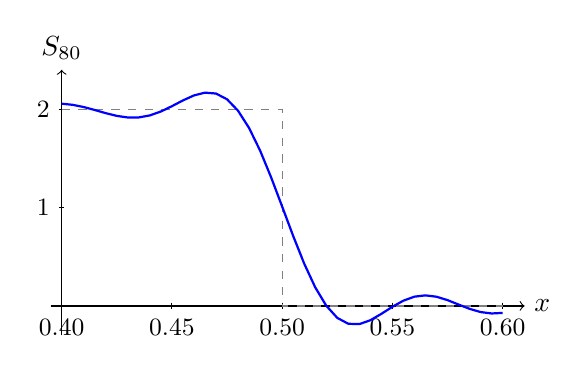
\begin{tikzpicture}[x=28cm,y=1.25cm]
\draw[->] (.395,0)--(.61,0) node[right]{$x$};
\draw[->] (.4,-.3)--(.4,2.4) node[above]{$S_{80}$};
\foreach \x/\lbl in {.4/0.40,.45/0.45,.5/0.50,.55/0.55,.6/0.60} {
 \draw (\x,.035)--(\x,-.035) node[below,font=\small]{$\lbl$};}
\foreach \y in {1,2} {
 \draw (.401,\y)--(.399,\y) node[left,font=\small]{$\y$};}
\draw[dashed,gray] (.4,2)--(.5,2)--(.5,0)--(.6,0);
\draw[blue,thick] plot coordinates {(0.400,2.0550217496) (0.405,2.0434445278) (0.410,2.0209666061) (0.415,1.9909228069) (0.420,1.9587255382) (0.425,1.9310739992) (0.430,1.9147899738) (0.435,1.9154450565) (0.440,1.9360026365) (0.445,1.9757226624) (0.450,2.0295599950) (0.455,2.0882266661) (0.460,2.1389909466) (0.465,2.1671654888) (0.470,2.1581122030) (0.475,2.0994848485) (0.480,1.9833622971) (0.485,1.8079117779) (0.490,1.5782694312) (0.495,1.3064319783) (0.500,1.0101041452) (0.505,0.7106182906) (0.510,0.4302063817) (0.515,0.1890300753) (0.520,0.0024369608) (0.525,-0.1211054656) (0.530,-0.1810437317) (0.535,-0.1845508447) (0.540,-0.1451340717) (0.545,-0.0802662162) (0.550,-0.0084458372) (0.555,0.0537999795) (0.560,0.0944412979) (0.565,0.1075546247) (0.570,0.0937421764) (0.575,0.0593150969) (0.580,0.0144351045) (0.585,-0.0293858766) (0.590,-0.0619021545) (0.595,-0.0763218939) (0.600,-0.0706167386)};
\end{tikzpicture}
\end{center}

The dashed line is the original step function; the solid line connects
all 41 requested computed values. On this grid the largest value is
$S_{80}(0.465)=2.1671654888\ldots$ and the smallest is
$S_{80}(0.535)=-0.1845508446\ldots$.
At the jump the partial sums tend to the midpoint value $1$: the same
computation gives $S_N(1/2)=1.0386$, $0.9893$, $1.0101$, $0.9972$,
$1.0026$ for $N=20$, $40$, $80$, $160$, $320$. The overshoot near the
jump, however, does not die out. On the grid
$x=0.40000(0.00001)0.50000$ (the same recurrence, in double precision)
the maximum of $S_{80}$ is $2.1690$, near $x=0.4665$, about $8.4\%$ of
the jump above $f=2$; for larger $N$ the maximum moves toward $x=1/2$,
while the overshoot approaches the Gibbs fraction of about $9\%$ of the
jump found for Fourier series in Section~19.3 ($S_{640}$ peaks at
$2.1797$ on the same grid). This is
the Gibbs phenomenon; it is not a failure of the exact coefficient
calculation.

\Needspace{5\baselineskip}
\par\bigskip
\noindent\textbf{15.2.24}\quad A plane wave may be expanded in a
series of spherical waves by the Rayleigh equation,
\[
e^{ikr\cos\gamma}=\sum_{n=0}^{\infty}a_{n}j_{n}(kr)P_{n}(\cos\gamma).
\]
Show that $a_{n}=i^{n}(2n+1)$.
\par\emph{Hint.}
\begin{enumerate}
\item[1.] Use the orthogonality of the $P_{n}$ to solve for
$a_{n}j_{n}(kr)$.
\item[2.] Differentiate $n$ times with respect to $(kr)$ and set
$r=0$ to eliminate the $r$-dependence.
\item[3.] Evaluate the remaining integral by Exercise~15.1.15.
\end{enumerate}
\par\emph{Note.}~This problem may also be treated by noting that both
sides of the equation satisfy the Helmholtz equation. The equality
can be established by showing that the solutions have the same
behavior at the origin and also behave alike at large distances.
\solution
Put $z=kr$ and $x=\cos\gamma$. Multiply the proposed expansion by
$P_n(x)$ and integrate over $-1\le x\le1$; by orthogonality,
$\int_{-1}^1P_mP_n\,dx=2\delta_{mn}/(2n+1)$, only the term $m=n$
survives:
\[
a_nj_n(z)=\frac{2n+1}{2}\int_{-1}^1e^{izx}P_n(x)dx.
\]
Expand $e^{izx}=\sum_{j\ge0}(iz)^jx^j/j!$; the series converges
uniformly for $-1\le x\le1$, so it may be integrated term by term.
All powers $x^j$ with $j<n$ have zero integral against $P_n$ by
Exercise 15.1.14, and for $j=n+1$ the integrand $x^{n+1}P_n$ is odd.
With the moment $\int_{-1}^1x^nP_n\,dx=2\cdot n!/(2n+1)!!$ of
Exercise 15.1.15, the right-hand side is therefore
\[
\frac{2n+1}{2}\frac{(iz)^n}{n!}
 \int_{-1}^1x^nP_n(x)dx+O(z^{n+2})
=\frac{(2n+1)i^nz^n}{(2n+1)!!}+O(z^{n+2}).
\]
The power series of $j_n$ (Section 14.7),
$j_n(z)=\sum_{k\ge0}(-1)^kz^{n+2k}/[2^kk!\,(2n+2k+1)!!]$, gives
$j_n(z)=z^n/(2n+1)!!+O(z^{n+2})$, so the left-hand side is
$a_nz^n/(2n+1)!!+O(z^{n+2})$. Comparing the coefficients of $z^n$ gives
\[
\boxed{a_n=i^n(2n+1)}.
\]
This is the procedure of the hint: differentiating both sides $n$ times
and setting $z=0$ removes all other terms and leaves
$a_n\,n!/(2n+1)!!=(2n+1)i^n\,n!/(2n+1)!!$; the common factor
$n!/(2n+1)!!$ cancels. Comparing power-series coefficients avoids any
division by $j_n(z)$, which has zeros. That the series with these
coefficients does sum to $e^{izx}$ is proved by the recurrence
argument in Exercise 15.2.25; Exercise 15.2.27 checks the coefficients
independently, by evaluating
$\frac{2n+1}2\int_{-1}^1e^{izx}P_n\,dx=i^n(2n+1)j_n(z)$ directly.

\Needspace{5\baselineskip}
\par\bigskip
\noindent\textbf{15.2.25}\quad Verify the Rayleigh equation of
Exercise~15.2.24 by starting with the following steps:
\begin{enumerate}
\item[(a)] Differentiate with respect to $(kr)$ to establish
\[
\sum_{n}a_{n}j'_{n}(kr)P_{n}(\cos\gamma)
=i\sum_{n}a_{n}j_{n}(kr)\cos\gamma\,P_{n}(\cos\gamma).
\]
\item[(b)] Use a recurrence relation to replace
$\cos\gamma\,P_{n}(\cos\gamma)$ by a linear combination of $P_{n-1}$
and $P_{n+1}$.
\item[(c)] Use a recurrence relation to replace $j'_{n}$ by a linear
combination of $j_{n-1}$ and $j_{n+1}$.
\end{enumerate}
\solution
Again put $z=kr$, $x=\cos\gamma$, and $F=\sum a_nj_n(z)P_n(x)$.
(a) If $F=e^{izx}$, then $F_z=ixF$. Differentiating the series term by
term (assumed in this derivation of the $a_n$; for the coefficients
found, it is justified in the sufficiency argument below) gives
$F_z=\sum_na_nj_n'(z)P_n(x)$, while
$ixF=i\sum_na_nj_n(z)\,xP_n(x)$; this is the displayed equation.

(b) Use the three-term recurrence
$xP_n=[(n+1)P_{n+1}+nP_{n-1}]/(2n+1)$:
\[
i\sum_na_nj_n\,xP_n
=i\sum_na_nj_n\left[\frac{n+1}{2n+1}P_{n+1}+\frac n{2n+1}P_{n-1}\right].
\]
A given $P_m$ comes from $n=m-1$ in the first term, with factor
$(n+1)/(2n+1)=m/(2m-1)$, and from $n=m+1$ in the second, with factor
$n/(2n+1)=(m+1)/(2m+3)$. So the coefficient of $P_m$ on the right is
\[
i\left[\frac{m\,a_{m-1}}{2m-1}j_{m-1}
+\frac{(m+1)a_{m+1}}{2m+3}j_{m+1}\right].
\]
The first term is absent for $m=0$.

(c) The spherical Bessel recurrence
$mj_{m-1}-(m+1)j_{m+1}=(2m+1)j_m'$ of Exercise 14.7.5 gives
\[
j_m'=\frac{m}{2m+1}j_{m-1}
-\frac{m+1}{2m+1}j_{m+1}
\]
for $m\ge1$; at $m=0$, where the coefficient of $j_{m-1}$ vanishes, it
reads $j_0'=-j_1$. Multiplying both sides of (a) by $P_m$ and
integrating over $-1\le x\le1$ (again term by term), orthogonality
shows that the coefficient $a_mj_m'$ of $P_m$ on the left must equal
the expression in (b). Inserting the recurrence and collecting terms,
\[
\left[\frac{m\,a_m}{2m+1}-\frac{i\,m\,a_{m-1}}{2m-1}\right]j_{m-1}
=\left[\frac{(m+1)a_m}{2m+1}+\frac{i(m+1)a_{m+1}}{2m+3}\right]j_{m+1}.
\]
Near $z=0$, $j_{m-1}$ and $j_{m+1}$ begin with the different powers
$z^{m-1}$ and $z^{m+1}$, so they are linearly independent and both
brackets vanish (for $m=0$ only the right one occurs). Dividing by $m$
and by $m+1$:
\[
\frac{a_m}{2m+1}=\frac{i\,a_{m-1}}{2m-1},\qquad
-\frac{a_m}{2m+1}=\frac{i\,a_{m+1}}{2m+3}.
\]
The first with $m$ replaced by $m+1$ reads $a_{m+1}/(2m+3)=ia_m/(2m+1)$;
the second, multiplied by $-i$ (and $-i\cdot i=1$), reads the same. So both
give the single recurrence $a_{m+1}=i(2m+3)a_m/(2m+1)$. Setting $z=0$
in the expansion, where $j_n(0)=\delta_{n0}$ and $P_0=1$, gives
$a_0=1$; and if $a_m=i^m(2m+1)$, then
$a_{m+1}=i(2m+3)i^m=i^{m+1}(2m+3)$. By induction $a_n=i^n(2n+1)$.

For sufficiency, insert these coefficients in $F$. The spherical
Bessel power series supplies a concrete uniform bound: for $|z|\le M$,
using $(2n+2k+1)!!\ge(2n+1)!!$,
\[
|j_n(z)|\le\sum_{k=0}^\infty
\frac{M^{n+2k}}{2^kk!(2n+2k+1)!!}
\le\frac{M^n}{(2n+1)!!}\sum_{k=0}^\infty\frac{(M^2/2)^k}{k!}
=\frac{M^n}{(2n+1)!!}e^{M^2/2}.
\]
After multiplication by $2n+1$, the ratio of consecutive bounds is
$M(2n-1)!!/(2n+1)!!=M/(2n+1)\to0$. Thus, by the ratio test and the
Weierstrass M test, $\sum(2n+1)|j_n(z)|$ converges uniformly on that
disk. The derivative recurrence above gives
$|j_n'|\le|j_{n-1}|+|j_{n+1}|$, hence the same conclusion for
$\sum(2n+1)|j_n'(z)|$, with $j_0'=-j_1$ handled separately.
Together with $|P_n(x)|\le1$, these bounds justify differentiating
$F$ term by term for $-1\le x\le1$.
The calculation above, read backwards, proves $F_z=ixF$. At zero,
$j_0(0)=1$ and $j_n(0)=0$ for $n>0$, so $F(0,x)=1$.
For fixed $x$, $\partial_z[e^{-izx}F]=e^{-izx}(F_z-ixF)=0$, so
$F(z,x)=F(0,x)e^{izx}=e^{izx}$, verifying the Rayleigh identity for all
finite $z$.

\Needspace{5\baselineskip}
\par\bigskip
\noindent\textbf{15.2.26}\quad From Exercise~15.2.24 show that
\[
j_{n}(kr)=\frac{1}{2i^{n}}\int_{-1}^{1}e^{ikr\mu}P_{n}(\mu)\,d\mu.
\]
This means that (apart from a constant factor) the spherical Bessel
function $j_{n}(kr)$ is an integral transform of the Legendre
polynomial $P_{n}(\mu)$.
\solution
Write the Rayleigh expansion of Exercise 15.2.24 with $z=kr$,
$\mu=\cos\gamma$ and $a_n=i^n(2n+1)$, multiply it by $P_m(\mu)$ and
integrate:
\[
\int_{-1}^1e^{iz\mu}P_m(\mu)d\mu
=\sum_{n\ge0}i^n(2n+1)j_n(z)
 \frac{2\delta_{nm}}{2n+1}
=2i^mj_m(z).
\]
Only $n=m$ survives, by the orthogonality relation
$\int_{-1}^1P_nP_m\,d\mu=2\delta_{nm}/(2n+1)$. Uniform convergence for
$\mu\in[-1,1]$ and fixed $z$ (Exercise 15.2.25: $\sum(2n+1)|j_n(z)|$
converges and $|P_n|\le1$) justifies the interchange of sum and
integral. Divide by $2i^m$ and rename the index:
\[
\boxed{j_n(z)=\frac1{2i^n}\int_{-1}^1e^{iz\mu}P_n(\mu)d\mu}.
\]
The integral is entire in $z$, so the formula also holds for complex
$z$ and at zero, with the usual removable values of $j_n$.

\Needspace{5\baselineskip}
\par\bigskip
\noindent\textbf{15.2.27}\quad Rewriting the formula of
Exercise~15.2.26 as
\[
j_{n}(z)=\frac{1}{2}(-i)^{n}\int_{0}^{\pi}e^{iz\cos\theta}
P_{n}(\cos\theta)\sin\theta\,d\theta,\qquad n=0,1,2,\ldots,
\]
verify it by transforming the right-hand side into
\[
\frac{z^{n}}{2^{n+1}n!}\int_{0}^{\pi}\cos(z\cos\theta)
\sin^{2n+1}\theta\,d\theta
\]
and using Exercise~14.7.9.
\solution
Call the right-hand side $I$. Put $x=\cos\theta$: then
$dx=-\sin\theta\,d\theta$, and $\theta=0,\pi$ become $x=1,-1$, so
reversing the limits absorbs the minus sign. Then insert Rodrigues'
formula, $P_n=D^n(x^2-1)^n/(2^nn!)$ with $D=d/dx$:
\[
I=\frac{(-i)^n}{2}\int_{-1}^1e^{izx}P_n(x)dx
=\frac{(-i)^n}{2^{n+1}n!}
 \int_{-1}^1e^{izx}D^n(x^2-1)^n dx.
\]
Integrate by parts $n$ times, moving one $D$ at a time onto the
exponential. As in Exercise 15.1.14, $D^k(x^2-1)^n$ vanishes at
$x=\pm1$ for $k<n$, so every boundary term vanishes, and since
$De^{izx}=ize^{izx}$ each step contributes a factor $-iz$:
\[
\int_{-1}^1e^{izx}D^n(x^2-1)^ndx
=(-iz)^n\int_{-1}^1e^{izx}(x^2-1)^ndx.
\]
Since $(-i)^n(-i)^n=(-1)^n$ and $(x^2-1)^n=(-1)^n(1-x^2)^n$, the two
signs cancel:
\[
I=\frac{z^n}{2^{n+1}n!}\int_{-1}^1e^{izx}(1-x^2)^n dx.
\]
Write $e^{izx}=\cos zx+i\sin zx$. The sine part is odd in $x$ and
integrates to zero, even for complex $z$. Returning to $\theta$ in the
cosine part ($1-x^2=\sin^2\theta$, $dx\to\sin\theta\,d\theta$ as
before) gives exactly
\[
I=\frac{z^n}{2^{n+1}n!}\int_0^\pi
\cos(z\cos\theta)\sin^{2n+1}\theta\,d\theta,
\]
the Poisson integral that Exercise 14.7.9 identifies with $j_n(z)$.
To verify the spherical Bessel value directly, expand
$\cos zx=\sum_k(-1)^kz^{2k}x^{2k}/(2k)!$ (uniformly convergent on
$[-1,1]$) and integrate each term; with $u=x^2$ on the even integrand,
\[
\int_{-1}^1x^{2k}(1-x^2)^ndx
=\int_0^1u^{k-1/2}(1-u)^n\,du
=B(k+\tfrac12,n+1)
=\frac{\Gamma(k+1/2)n!}{\Gamma(k+n+3/2)}.
\]
With $\Gamma(k+\frac12)=(2k)!\sqrt\pi/(4^kk!)$ and
$\Gamma(k+n+\frac32)=(2n+2k+1)!!\sqrt\pi/2^{k+n+1}$, the $k$th term of
$I$ is
\[
\frac{z^n}{2^{n+1}n!}\,\frac{(-1)^kz^{2k}}{(2k)!}\,
\frac{(2k)!\,n!}{4^kk!}\,\frac{2^{k+n+1}}{(2n+2k+1)!!}
=\frac{(-1)^kz^{n+2k}}{2^kk!\,(2n+2k+1)!!}.
\]
Therefore
\[
I=\sum_{k=0}^\infty
\frac{(-1)^kz^{n+2k}}{2^kk!(2n+2k+1)!!}=j_n(z),
\]
the power series of $j_n$ (Section 14.7). This reproduces the
Poisson representation of Exercise 14.7.9 without assuming it.

\Needspace{8\baselineskip}
\subsection*{15.3 Physical Interpretation of Generating Function}

\Needspace{5\baselineskip}
\par\bigskip
\noindent\textbf{15.3.1}\quad Develop the electrostatic potential for
the array of charges shown in Fig.~15.7. This is a linear electric
quadrupole.
\solution
In Fig.~15.7 the charges are $q,-2q,q$ at $z=-a,0,a$.
Coulomb's law therefore gives, at every point away from these charges,
\[
V=\frac{q}{4\pi\varepsilon_0}
\left[\frac1{\sqrt{r^2+a^2+2ar\cos\theta}}-\frac2r
+\frac1{\sqrt{r^2+a^2-2ar\cos\theta}}\right].
\]
For $r>a$, expand the two displaced charges with the generating
function, $t=\pm a/r$:
\[
\frac1{\sqrt{r^2+a^2\mp2ar\cos\theta}}
=\frac1r\Bigl[1\mp2\frac ar\cos\theta+\frac{a^2}{r^2}\Bigr]^{-1/2}
=\sum_{n=0}^\infty\frac{(\pm a)^n}{r^{n+1}}P_n(\cos\theta).
\]
Their $n$th coefficients add to $1+(-1)^n$, which is $0$ for odd $n$
and $2$ for even $n$. The $n=0$ term, $2/r$, cancels the central
charge's $-2/r$, and $n=2s$ leaves $2a^{2s}/r^{2s+1}$:
\[
\boxed{V=\frac{2q}{4\pi\varepsilon_0r}
\sum_{s=1}^\infty\left(\frac ar\right)^{2s}P_{2s}(\cos\theta)}.
\]
In particular,
\[
V=\frac{2qa^2}{4\pi\varepsilon_0r^3}P_2(\cos\theta)
+O(a^4/r^5)
=\frac{qa^2(3\cos^2\theta-1)}{4\pi\varepsilon_0r^3}
+O(a^4/r^5).
\]
The total charge and dipole moment are zero, while
$\sum q_i z_i^2=2qa^2\ne0$, identifying the leading quadrupole.

\Needspace{5\baselineskip}
\par\bigskip
\noindent\textbf{15.3.2}\quad Calculate the electrostatic potential of
the array of charges shown in Fig.~15.8. Here is an example of two
equal but oppositely directed quadrupoles. The quadrupole
contributions cancel. The octopole terms do not cancel.
\solution
Figure 15.8 has charges $-q,2q,-2q,q$ at $-2a,-a,a,2a$.
Thus the exact potential is
\[
V=\frac{q}{4\pi\varepsilon_0}
\left[-\frac1{|\mathbf r+2a\hat{\mathbf z}|}
+\frac2{|\mathbf r+a\hat{\mathbf z}|}
-\frac2{|\mathbf r-a\hat{\mathbf z}|}
+\frac1{|\mathbf r-2a\hat{\mathbf z}|}\right].
\]
For $r>2a$, expand each term with the generating function,
$1/|\mathbf r-c\hat{\mathbf z}|=\sum_nc^nP_n(\cos\theta)/r^{n+1}$ for
$|c|<r$, with $c=-2a,-a,a,2a$. The coefficient of
$(q/4\pi\varepsilon_0)a^nP_n(\cos\theta)/r^{n+1}$ is
\[
-(-2)^n+2(-1)^n-2+2^n
=[1-(-1)^n](2^n-2).
\]
For even $n$ the four terms cancel in pairs; for odd $n$ they give
$2^{n+1}-4=2(2^n-2)$. So the coefficient is zero for every even $n$ and
also for $n=1$. Putting $n=2s+1$ leaves
\[
\boxed{V=\frac{2q}{4\pi\varepsilon_0r}
\sum_{s=1}^\infty(2^{2s+1}-2)
\left(\frac ar\right)^{2s+1}P_{2s+1}(\cos\theta)}.
\]
The leading term ($s=1$, with $2^3-2=6$) is
\[
\boxed{V_{\rm oct}=\frac{12qa^3}{4\pi\varepsilon_0r^4}
P_3(\cos\theta)}.
\]
This also follows from the axial moments $\mu_n=\sum_iq_iz_i^n$, in
terms of which the same expansion reads
$V=\sum_n\mu_nP_n(\cos\theta)/(4\pi\varepsilon_0r^{n+1})$:
$\mu_0=\mu_1=\mu_2=0$ and
$\mu_3=q[-(-2)^3+2(-1)^3-2+2^3]a^3=q[8-2-2+8]a^3=12qa^3$.

\Needspace{5\baselineskip}
\par\bigskip
\noindent\textbf{15.3.3}\quad Show that the electrostatic potential
produced by a charge $q$ at $z=a$ for $r<a$ is
\[
\varphi(r)=\frac{q}{4\pi\varepsilon_{0}a}
\sum_{n=0}^{\infty}\left(\frac{r}{a}\right)^{n}P_{n}(\cos\theta).
\]
\solution
The source-point distance is
$|\mathbf r-a\hat{\mathbf z}|=\sqrt{a^2+r^2-2ar\cos\theta}$.
For $0\le r<a$, factor out $a$ and use the generating function with
$t=r/a$:
\[
\varphi=\frac{q}{4\pi\varepsilon_0a}
\left[1-2\frac ra\cos\theta+\left(\frac ra\right)^2\right]^{-1/2}
=\boxed{\frac{q}{4\pi\varepsilon_0a}
\sum_{n=0}^\infty\left(\frac ra\right)^nP_n(\cos\theta)}.
\]
For each fixed $r<a$ the series converges uniformly in $\theta$, since
$|P_n(\cos\theta)|\le1$ bounds its terms by those of the geometric
series $\sum_n(r/a)^n$. At $r=0$ the value is
$q/(4\pi\varepsilon_0a)$, with all higher terms vanishing.

\Needspace{5\baselineskip}
\par\bigskip
\noindent\textbf{15.3.4}\quad Using $\mathbf{E}=-\nabla\varphi$,
determine the components of the electric field corresponding to the
(pure) electric dipole potential,
\[
\varphi(r)=\frac{2aq\,P_{1}(\cos\theta)}{4\pi\varepsilon_{0}r^{2}}.
\]
Here it is assumed that $r\gg a$.
\par\nobreak\hfill\emph{ANS.}\enspace
$E_{r}=+\dfrac{4aq\cos\theta}{4\pi\varepsilon_{0}r^{3}}$,\quad
$E_{\theta}=+\dfrac{2aq\sin\theta}{4\pi\varepsilon_{0}r^{3}}$,\quad
$E_{\varphi}=0$.
\solution
Since $P_1(\cos\theta)=\cos\theta$, put $C=2aq/(4\pi\varepsilon_0)$
and write $\varphi=C r^{-2}\cos\theta$.
The spherical gradient gives
\[
E_r=-\partial_r\varphi=2Cr^{-3}\cos\theta,\qquad
E_\theta=-\frac1r\partial_\theta\varphi=Cr^{-3}\sin\theta,
\qquad E_\varphi=-\frac1{r\sin\theta}\partial_\varphi\varphi=0.
\]
Substituting $C$ yields all three stated components. For a pair of
charges separated by $2a$ these are its leading $r\gg a$ terms;
for an ideal point dipole of fixed moment $2aq$ they are exact at $r>0$.

\Needspace{5\baselineskip}
\par\bigskip
\noindent\textbf{15.3.5}\quad Operating in spherical polar
coordinates, show that \erratum{for $r>0$}
\[
\frac{\partial}{\partial z}\left[\frac{P_{l}(\cos\theta)}{r^{l+1}}\right]
=-(l+1)\frac{P_{l+1}(\cos\theta)}{r^{l+2}}.
\]
This is the key step in the mathematical argument that the derivative
of one multipole leads to the next higher multipole.
\par\emph{Hint.}~Compare with Exercise~3.10.28.
\solution
At fixed Cartesian $x,y$, write $\rho=\sqrt{x^2+y^2}$,
$r=\sqrt{\rho^2+z^2}$ and $u=z/r=\cos\theta$. Then
\[
\frac{\partial r}{\partial z}=\frac zr=u,\qquad
\frac{\partial u}{\partial z}=\frac1r-\frac z{r^2}\frac{\partial r}{\partial z}
=\frac1r-\frac{z^2}{r^3}=\frac{1-u^2}{r}.
\]
Hence, by the product and chain rules,
\begin{align*}
\partial_z\!\left[r^{-l-1}P_l(u)\right]
&=-(l+1)r^{-l-2}u\,P_l(u)+r^{-l-1}P_l'(u)\frac{1-u^2}r\\
&=r^{-l-2}\left[-(l+1)uP_l(u)+(1-u^2)P_l'(u)\right].
\end{align*}
Exercise 15.1.7 gives
$(1-u^2)P_l'=(l+1)(uP_l-P_{l+1})$.
The $uP_l$ terms cancel, leaving
\[
\boxed{\partial_z\!\left[\frac{P_l(\cos\theta)}{r^{l+1}}\right]
=-(l+1)\frac{P_{l+1}(\cos\theta)}{r^{l+2}}},\qquad r>0.
\]
Both sides are singular at the origin, where $\theta$ is undefined;
hence the restriction $r>0$ added to the statement.
This chain-rule calculation is equivalent to
$\partial_z=\cos\theta\,\partial_r-(\sin\theta/r)\partial_\theta$.

\Needspace{5\baselineskip}
\par\bigskip
\noindent\textbf{15.3.6}\quad A point electric dipole of strength
$p^{(1)}$ is placed at $z=a$; a second point electric dipole of equal
but opposite strength is at the origin. Keeping the product
$p^{(1)}a$ constant, let $a\to0$. Show that this results in a point
electric quadrupole.
\par\emph{Hint.}~Exercise~15.3.5 (when proved) will be helpful.
\solution
Define $F_1(\mathbf r)=P_1(\cos\theta)/r^2$.
The positive $z$ dipole at $a\hat{\mathbf z}$ and its negative at zero
have combined potential
\[
V_a(\mathbf r)=\frac{p^{(1)}}{4\pi\varepsilon_0}
[F_1(\mathbf r-a\hat{\mathbf z})-F_1(\mathbf r)].
\]
At each fixed point away from the origin, Taylor expansion in $a$ gives
$F_1(\mathbf r-a\hat{\mathbf z})-F_1(\mathbf r)
=-a\,\partial_zF_1+O(a^2)$.
Exercise 15.3.5 with $l=1$ evaluates $\partial_zF_1=-2P_2/r^3$, so
\[
V_a=\frac{p^{(1)}}{4\pi\varepsilon_0}
\left[\frac{2aP_2(\cos\theta)}{r^3}+O(a^2)\right]
=\frac{2p^{(1)}a\,P_2(\cos\theta)}{4\pi\varepsilon_0r^3}
+p^{(1)}O(a^2).
\]
Holding $K=p^{(1)}a$ fixed, the error is $p^{(1)}O(a^2)=O(Ka)\to0$, so
\[
\boxed{V_{\rm quad}=\frac{2K}{4\pi\varepsilon_0r^3}
P_2(\cos\theta)}.
\]
In the convention $V_{\rm quad}=p^{(2)}P_2/(4\pi\varepsilon_0r^3)$,
the resulting quadrupole strength is $p^{(2)}=2ap^{(1)}$.
The dipole terms cancel, while a nonzero $r^{-3}P_2$ term remains.

\Needspace{5\baselineskip}
\par\bigskip
\noindent\textbf{15.3.7}\quad A point electric octupole may be
constructed by placing a point electric quadrupole (pole strength
$p^{(2)}$ in the $z$-direction) at $z=a$ and an equal but opposite
point electric quadrupole at $z=0$ and then letting $a\to0$, subject
to $p^{(2)}a=\mathrm{constant}$. Find the electrostatic potential
corresponding to a point electric octupole. Show from the
construction of the point electric octupole that the corresponding
potential may be obtained by differentiating the point quadrupole
potential.
\solution
Use the same strength convention:
$V^{(2)}=p^{(2)}P_2(\cos\theta)/(4\pi\varepsilon_0r^3)$.
For a positive quadrupole displaced to $z=a$ and its negative at zero,
\[
V_a^{(3)}=\frac{p^{(2)}}{4\pi\varepsilon_0}
\left[F_2(\mathbf r-a\hat{\mathbf z})-F_2(\mathbf r)\right],
\qquad F_2=\frac{P_2(\cos\theta)}{r^3}.
\]
The Taylor difference is $-a\partial_zF_2+O(a^2)$, and
Exercise 15.3.5 with $l=2$ gives $\partial_zF_2=-3P_3/r^4$, so
$V_a^{(3)}=3ap^{(2)}P_3/(4\pi\varepsilon_0r^4)+p^{(2)}O(a^2)$.
Therefore, keeping $K_2=ap^{(2)}$ fixed and using
$P_3=\frac12(5\cos^3\theta-3\cos\theta)$,
\[
\boxed{V^{(3)}=\frac{3K_2}{4\pi\varepsilon_0r^4}P_3(\cos\theta)
=\frac{3K_2}{8\pi\varepsilon_0r^4}(5\cos^3\theta-3\cos\theta)}.
\]
Thus $p^{(3)}=3ap^{(2)}$ in this convention, and the construction
is precisely $V^{(3)}=-a\,\partial_zV^{(2)}$ in the limiting sense.
The sign is set by putting the positive source at $+a$.
\erratum{The Instructor's Manual, p.~245, instead writes $48a^3q$ for
the numerator of the octupole moment, although this exercise supplies
$p^{(2)}$, not a charge $q$. In the stated strength convention the
moment is $3ap^{(2)}$. That form would agree only after the
additional, unstated assignment $p^{(2)}=16a^2q$.}

\Needspace{5\baselineskip}
\par\bigskip
\noindent\textbf{15.3.8}\quad A point charge $q$ is in the interior of
a hollow conducting sphere of radius $r_{0}$. The charge $q$ is
displaced a distance \erratum{$0<a<r_0$} from the center of the sphere. If the
conducting sphere is grounded, show that the potential in the
interior produced by $q$ and the distributed induced charge is the
same as that produced by $q$ and its image charge $q'$. The image
charge is at a distance $a'=r_{0}^{2}/a$ from the center, collinear
with $q$ and the origin (Fig.~15.9).
\par\emph{Hint.}~Calculate the electrostatic potential for
$a<r_{0}<a'$. Show that the potential vanishes for $r=r_{0}$ if we
take $q'=-qr_{0}/a$.
\solution
For $0<a<r_0$, place $q'=-qr_0/a$ at $a'=r_0^2/a>r_0$.
The restriction added to the statement is needed: for $a=0$ there is
no image point $a'$ (that case is treated as a limit at the end), and
$a<r_0$ puts $q$ inside the sphere and its image outside.
Consider
\[
V(\mathbf r)=\frac1{4\pi\varepsilon_0}
\left[\frac q{|\mathbf r-a\hat{\mathbf z}|}
-\frac{qr_0/a}{|\mathbf r-a'\hat{\mathbf z}|}\right].
\]
On $r=r_0$, $|\mathbf r-a\hat{\mathbf z}|^2=r_0^2+a^2-2ar_0\cos\theta$,
and the two distances satisfy
\[
|\mathbf r-a'\hat{\mathbf z}|^2
=r_0^2+\frac{r_0^4}{a^2}-\frac{2r_0^3}{a}\cos\theta
=\frac{r_0^2}{a^2}|\mathbf r-a\hat{\mathbf z}|^2.
\]
Their positive square roots therefore satisfy
$|\mathbf r-a'\hat{\mathbf z}|=(r_0/a)|\mathbf r-a\hat{\mathbf z}|$,
and the two potential terms cancel exactly.

The Legendre version of the same cancellation uses expansions valid
for $a<r<a'$, a range that contains the sphere $r=r_0$.
There $r>a$ and $r<a'$, so the generating function gives
$1/|\mathbf r-a\hat{\mathbf z}|=\sum_na^nP_n/r^{n+1}$ and
$1/|\mathbf r-a'\hat{\mathbf z}|=\sum_nr^nP_n/(a')^{n+1}$ (as in
Exercise 15.3.3), hence
\[
V=\frac1{4\pi\varepsilon_0}\sum_{n=0}^\infty
\left[\frac{qa^n}{r^{n+1}}+
\frac{q'r^n}{(a')^{n+1}}\right]P_n(\cos\theta).
\]
At $r=r_0$, inserting $q'=-qr_0/a$ and
$(a')^{n+1}=r_0^{2n+2}/a^{n+1}$ makes each bracket zero:
\[
\frac{q'r_0^n}{(a')^{n+1}}
=-\frac{qr_0}a\,\frac{r_0^n\,a^{n+1}}{r_0^{2n+2}}
=-\frac{qa^n}{r_0^{n+1}}.
\]
The image term is harmonic everywhere inside the sphere, because its
source is outside; the real charge has exactly the required Coulomb
singularity. The difference from any other grounded solution is
harmonic, including across the canceled source singularity, and zero
on the boundary. Uniqueness for the Dirichlet problem proves the result
throughout the interior, including $r<a$, where the first expansion
diverges.
For $a=0$, take the limit directly: as $a\to0$, $a'\to\infty$ and the
image term tends to $-(qr_0/a)/a'=-q/r_0$, so
$V=q(1/r-1/r_0)/(4\pi\varepsilon_0)$.

\Needspace{8\baselineskip}
\subsection*{15.4 Associated Legendre Equation}

\Needspace{5\baselineskip}
\par\bigskip
\noindent\textbf{15.4.1}\quad Apply the Frobenius method to
Eq.~(15.72) to obtain Eq.~(15.73) and verify that the numerator of
that equation becomes zero if $\lambda=l(l+1)$ and $j=l-m$.
\solution
Write $U$ for the factor multiplying $(1-x^2)^{m/2}$ in the associated
Legendre function; Eq. (15.72) is
\[
(1-x^2)U''-2(m+1)xU'+[\lambda-m(m+1)]U=0.
\]
For $U=\sum_{j\ge0}a_jx^{j+k}$, the lowest power $x^{k-2}$
has coefficient $k(k-1)a_0$, so $k=0$ or $1$.
The next power, $x^{k-1}$, has coefficient $k(k+1)a_1$.
Thus $k=1$ forces $a_1=0$, whereas $k=0$ leaves $a_0,a_1$
independent; these are the even and odd branches at the ordinary
point $x=0$.
In general, $x^{j+k}$ receives
$(j+k+2)(j+k+1)a_{j+2}-(j+k)(j+k-1)a_j$ from $(1-x^2)U''$ (the first
part from the term $a_{j+2}x^{j+k+2}$), $-2(m+1)(j+k)a_j$ from
$-2(m+1)xU'$, and $[\lambda-m(m+1)]a_j$ from the last term. So the
coefficient of $x^{j+k}$ is
\[
(j+k+2)(j+k+1)a_{j+2}
+\{\lambda-m(m+1)-(j+k)(j+k-1)-2(m+1)(j+k)\}a_j.
\]
Set it to zero, using
$(j+k)(j+k-1)+2(m+1)(j+k)=(j+k)^2+(2m+1)(j+k)$:
\[
a_{j+2}=
\frac{(j+k)^2+(2m+1)(j+k)-\lambda+m(m+1)}
{(j+k+1)(j+k+2)}a_j.
\]
For $k=0$ the numerator is $j^2+(2m+1)j+m(m+1)-\lambda
=(j+m)(j+m+1)-\lambda$, and this is exactly Eq. (15.73).
If $\lambda=l(l+1)$, put $p=j+m$; the numerator factors as
\[
p(p+1)-l(l+1)=(p-l)(p+l)+(p-l)=(j+m-l)(j+m+l+1),
\]
which vanishes at $j=l-m$. The parity of $l-m$ selects the even
or odd power series. For nonnegative integers $m\le l$, that branch
terminates in a polynomial of degree $l-m$.

\Needspace{5\baselineskip}
\par\bigskip
\noindent\textbf{15.4.2}\quad Starting from the entries for $P_{2}^{2}$
and $P_{2}^{1}$ in Table~15.3, apply a recurrence formula to obtain
$P_{2}^{0}$ (which is $P_{2}$), $P_{2}^{-1}$, and $P_{2}^{-2}$.
Compare your results with the value of $P_{2}$ from Table~15.1 and
with values of $P_{2}^{-1}$ and $P_{2}^{-2}$ obtained by applying
Eq.~(15.81) to entries from Table~15.3.
\solution
Put $s=\sqrt{1-x^2}$ on $-1<x<1$.
Table 15.3 gives $P_2^2=3(1-x^2)=3s^2$ and $P_2^1=-3xs$.
Use the fixed-degree recurrence of Exercise 15.4.8 with $l=2$, so
that $l(l+1)=6$:
\[
P_2^{m+1}+\frac{2mx}{s}P_2^m+[6-m(m-1)]P_2^{m-1}=0.
\]
At $m=1$, this gives
$3s^2+\frac{2x}{s}(-3xs)+6P_2^0=3s^2-6x^2+6P_2^0=0$, so
$P_2^0=x^2-\frac12(1-x^2)$, i.e.
\[
\boxed{P_2^0=\frac{3x^2-1}{2}},
\]
which is $P_2$ of Table 15.1.
At $m=0$ the middle term is absent and $6-0=6$:
$P_2^1+6P_2^{-1}=0$, so
\[
\boxed{P_2^{-1}=-\frac16(-3xs)=\frac12xs}.
\]
At $m=-1$, $6-(-1)(-2)=4$ and
$P_2^0-(2x/s)P_2^{-1}+4P_2^{-2}=0$.
Substituting the two results, $(2x/s)(xs/2)=x^2$ and
$4P_2^{-2}=x^2-(3x^2-1)/2=(1-x^2)/2=s^2/2$, so
\[
\boxed{P_2^{-2}=\frac18(1-x^2)}.
\]
For the comparison the exercise asks for, Eq. (15.81),
$P_l^{-m}=(-1)^m[(l-m)!/(l+m)!]P_l^m$, applied to the Table 15.3
entries predicts
$P_2^{-1}=-(1!/3!)P_2^1=xs/2$ and
$P_2^{-2}=(0!/4!)P_2^2=3s^2/24=s^2/8$, in agreement.
(For $P_2^{-1}$ and $P_2^{-2}$ this is a consistency check rather than
an independent derivation, since Exercise 15.4.8 proves the recurrence
for $m\le0$ from Eq. (15.81), in the form of Exercise 15.4.3.)
The endpoint values follow by continuity.

\Needspace{5\baselineskip}
\par\bigskip
\noindent\textbf{15.4.3}\quad Prove that, \erratum{for integers $0\le m\le l$ and
$-1<x<1$},
\[
P_{l}^{-m}(x)=(-1)^{m}\frac{(l-m)!}{(l+m)!}\,P_{l}^{m}(x),
\]
where $P_{l}^{m}(x)$ is defined by
\[
P_{l}^{m}(x)=\frac{(-1)^{m}}{2^{l}l!}(1-x^{2})^{m/2}
\frac{d^{l+m}}{dx^{l+m}}(x^{2}-1)^{l}.
\]
\par\emph{Hint.}~One approach is to apply Leibniz's formula to
$(x+1)^{l}(x-1)^{l}$.
\solution
Let $F=(x-1)^l(x+1)^l$, $D=d/dx$, and take integers $0\le m\le l$.
Leibniz's rule, $D^N(fg)=\sum_i\binom Ni D^if\,D^{N-i}g$, with
$D^i(x\mp1)^l=\frac{l!}{(l-i)!}(x\mp1)^{l-i}$ for $i\le l$ (and zero for
$i>l$), gives for $N=l-m$, with $i=j$,
\[
D^{l-m}F=\sum_{j=0}^{l-m}
\frac{(l-m)!(l!)^2(x-1)^{l-j}(x+1)^{m+j}}
{j!(l-m-j)!(l-j)!(m+j)!}.
\]
For $D^{l+m}F$, the number $i$ of derivatives on the first factor
must lie between $m$ and $l$, because neither factor survives more than
$l$ derivatives. Write $i=m+j$, so the second factor receives $l-j$
derivatives:
\[
D^{l+m}F=\sum_{j=0}^{l-m}
\frac{(l+m)!(l!)^2(x-1)^{l-m-j}(x+1)^j}
{(m+j)!(l-j)!(l-m-j)!j!}.
\]
Multiplication of the second sum by $(x^2-1)^m=(x-1)^m(x+1)^m$ makes
its powers $(x-1)^{l-j}(x+1)^{m+j}$, exactly those of the first sum.
The remaining factors $(l!)^2/[j!(l-m-j)!(l-j)!(m+j)!]$ are the same in
both sums, so the coefficients differ only by the ratio
$(l-m)!/(l+m)!$. Thus
\[
D^{l-m}F=\frac{(l-m)!}{(l+m)!}(x^2-1)^mD^{l+m}F.
\]
Insert this identity into the Rodrigues definition with order $-m$,
where $(-1)^{-m}=(-1)^m$ and $(x^2-1)^m=(-1)^m(1-x^2)^m$:
\begin{align*}
P_l^{-m}
&=\frac{(-1)^m}{2^ll!}(1-x^2)^{-m/2}
 \frac{(l-m)!}{(l+m)!}(-1)^m(1-x^2)^mD^{l+m}F\\
&=(-1)^m\frac{(l-m)!}{(l+m)!}\,
 \frac{(-1)^m}{2^ll!}(1-x^2)^{m/2}D^{l+m}F
=\boxed{(-1)^m\frac{(l-m)!}{(l+m)!}P_l^m}.
\end{align*}
On $(-1,1)$ choose the positive square root of $1-x^2$.
The restrictions added to the statement are needed: for $m>l$ the
definition of $P_l^{-m}$ would require a derivative of negative order
$l-m$, and $(l-m)!$ is undefined; at $x=\pm1$ its factor
$(1-x^2)^{-m/2}$ is undefined for $m\ge1$, although both sides extend
continuously there. (Orders $-l\le m<0$ give the same identity solved
for $P_l^{|m|}$.)
The identity also extends with any consistently chosen complex branch.

\Needspace{5\baselineskip}
\par\bigskip
\noindent\textbf{15.4.4}\quad Show that
\begin{align*}
P_{2l}^{1}(0)&=0,\\
P_{2l+1}^{1}(0)&=(-1)^{l+1}\frac{(2l+1)!!}{(2l)!!},
\end{align*}
by each of these three methods:
\begin{enumerate}
\item[(a)] Use of recurrence relations,
\item[(b)] Expansion of the generating function,
\item[(c)] Rodrigues formula.
\end{enumerate}
\solution
Write the index of the statement as $s$, so the claims are
$P_{2s}^1(0)=0$ and $P_{2s+1}^1(0)=(-1)^{s+1}(2s+1)!!/(2s)!!$.

(a) The fixed-order recurrence
$(2l+1)xP_l^m=(l+m)P_{l-1}^m+(l-m+1)P_{l+1}^m$ (also used in
Exercise 15.4.12) at $x=0$, with $m=1$, gives
\[
lP_{l+1}^1(0)=-(l+1)P_{l-1}^1(0),\qquad l\ge1.
\]
The starting values are $P_0^1(0)=0$ and $P_1^1(0)=-1$, from
$P_0^1=0$ and $P_1^1=-\sqrt{1-x^2}$.
Odd $l$ link the even indices, so every even-index value is zero.
For the odd subsequence, $l=2k$ gives
$P_{2k+1}^1(0)=-\frac{2k+1}{2k}P_{2k-1}^1(0)$; using
$k=1,2,\ldots,s$ in turn,
\[
P_{2s+1}^1(0)=(-1)^s\frac{3\cdot5\cdots(2s+1)}
{2\cdot4\cdots2s}P_1^1(0)
=\boxed{(-1)^{s+1}\frac{(2s+1)!!}{(2s)!!}}.
\]

(b) Differentiate the generating function
$\sum_lP_l(x)t^l=(1-2xt+t^2)^{-1/2}$ with respect to $x$:
$\sum_lP_l'(x)t^l=t(1-2xt+t^2)^{-3/2}$. At $x=0$,
$P_l^1(0)=-\sqrt{1-0}\,P_l'(0)=-P_l'(0)$, so the binomial series
gives
\[
\sum_{l\ge0}P_l^1(0)t^l=-t(1+t^2)^{-3/2}
=-\sum_{s\ge0}(-1)^s\frac{(2s+1)!!}{2^ss!}t^{2s+1},
\]
because
\[
\binom{-3/2}{s}=\frac{(-\frac32)(-\frac52)\cdots(-\frac{2s+1}2)}{s!}
=(-1)^s\frac{(2s+1)!!}{2^ss!}.
\]
There are no even powers, and $2^ss!=(2s)!!$, so the coefficient of
$t^{2s+1}$ is $(-1)^{s+1}(2s+1)!!/(2s)!!$: the same values.

(c) Since $P_n^1(0)=-P_n'(0)$, which is minus the coefficient of $x$
in $P_n$, Rodrigues' formula gives
\[
P_n^1(0)=-\frac1{2^nn!}D^{n+1}(x^2-1)^n\Big|_{x=0},\qquad
(x^2-1)^n=\sum_{k=0}^n\binom nk(-1)^{n-k}x^{2k}.
\]
At $x=0$, $D^{n+1}x^{2k}$ is nonzero only for $2k=n+1$, when it equals
$(n+1)!$. For $n=2s$ no such $k$ exists, so $P_{2s}^1(0)=0$. For
$n=2s+1$ the term is $k=s+1$, with $(-1)^{n-k}=(-1)^s$:
\[
P_{2s+1}^1(0)=-\frac{(-1)^s}{2^{2s+1}(2s+1)!}
\binom{2s+1}{s+1}(2s+2)!
=(-1)^{s+1}\frac{(2s+2)!}{2^{2s+1}s!\,(s+1)!}.
\]
With $(2s+2)!=(2s+1)!!\,(2s+2)!!=(2s+1)!!\,2^{s+1}(s+1)!$ this is
$(-1)^{s+1}(2s+1)!!/(2^ss!)=(-1)^{s+1}(2s+1)!!/(2s)!!$.
This proves both formulas by the third requested method.

\Needspace{5\baselineskip}
\par\bigskip
\noindent\textbf{15.4.5}\quad Evaluate $P_{l}^{m}(0)$ for \erratum{integers $-l\le m\le l$}.
\par\nobreak\hfill\emph{ANS.}\enspace
$P_{l}^{m}(0)=\begin{cases}
(-1)^{(l+m)/2}\dfrac{(l+m-1)!!}{(l-m)!!}, & l+m\text{ even},\\[10pt]
0, & l+m\text{ odd}.
\end{cases}$
\solution
For integers $0\le m\le l$, the definition
$P_l^m=(-1)^m(1-x^2)^{m/2}D^mP_l$ ($D=d/dx$) gives
$P_l^m(0)=(-1)^mP_l^{(m)}(0)$, and by Taylor's formula
$P_l^{(m)}(0)=m!\,c_m$, where $c_m$ is the coefficient of $x^m$ in $P_l$.
The powers in $P_l$ are $l,l-2,\ldots$ (Exercise 15.1.2), so $c_m=0$
when $l+m$ is odd.
If $l+m$ is even, the power $x^{l-2k}=x^m$ of Exercise 15.1.2 has
$k=(l-m)/2$, so that $2l-2k=l+m$, $l-k=(l+m)/2$ and $l-2k=m$:
\[
c_m=(-1)^{(l-m)/2}\frac{(l+m)!}{2^l[(l-m)/2]!\,[(l+m)/2]!\,m!}.
\]
Multiplying by $(-1)^mm!$ and using
$(-1)^m(-1)^{(l-m)/2}=(-1)^{(l+m)/2}$ gives
\[
P_l^m(0)=
(-1)^{(l+m)/2}
\frac{(l+m)!}{2^l[(l-m)/2]![(l+m)/2]!}.
\]
Write $2^l=2^{(l+m)/2}\,2^{(l-m)/2}$ and split the factorials into even
and odd factors, $(l+m)!=(l+m)!!\,(l+m-1)!!$ with
$(l+m)!!=2^{(l+m)/2}[(l+m)/2]!$:
\[
\frac{(l+m)!}{2^{(l+m)/2}[(l+m)/2]!}=(l+m-1)!!,\qquad
2^{(l-m)/2}[(l-m)/2]!=(l-m)!!.
\]
Hence the stated nonzero value is
\[
\boxed{P_l^m(0)=(-1)^{(l+m)/2}\frac{(l+m-1)!!}{(l-m)!!}}.
\]
For $m=0$ this is $P_l(0)=(-1)^{l/2}(l-1)!!/l!!$ for even $l$, as in
Exercise 15.1.12, and $m=1$ reproduces Exercise 15.4.4.

Negative orders need no separate formula. For $m=-\mu$ with
$1\le\mu\le l$, Exercise 15.4.3 gives
$P_l^{-\mu}(0)=(-1)^\mu\frac{(l-\mu)!}{(l+\mu)!}P_l^\mu(0)$, which
vanishes when $l+\mu$, and hence $l+m=l-\mu$, is odd. Otherwise, by
$(l-\mu)!/(l-\mu)!!=(l-\mu-1)!!$, $(l+\mu)!/(l+\mu-1)!!=(l+\mu)!!$ and
$(-1)^{\mu+(l+\mu)/2}=(-1)^{(l-\mu)/2+2\mu}=(-1)^{(l-\mu)/2}$,
\[
P_l^{-\mu}(0)=(-1)^\mu\frac{(l-\mu)!}{(l+\mu)!}\,
(-1)^{(l+\mu)/2}\frac{(l+\mu-1)!!}{(l-\mu)!!}
=(-1)^{(l-\mu)/2}\frac{(l-\mu-1)!!}{(l+\mu)!!},
\]
which is the boxed formula with $m=-\mu$.
The restriction $|m|\le l$ in the statement is needed: for integer
$m>l$ the defining derivative makes $P_l^m=0$, while for even $l+m$ the
factorial expression would contain $(l-m)!!$ with $l-m<0$; for $m<-l$
the Rodrigues definition would require a derivative of negative order
$l+m$.

\Needspace{5\baselineskip}
\par\bigskip
\noindent\textbf{15.4.6}\quad Starting from the potential of a finite
dipole, Eq.~(15.65), verify the formulas for the electric field
components given as Eqs.~(15.130) and (15.131).
\solution
For charges $\pm q$ at $z=\pm a$,
$V=(q/4\pi\varepsilon_0)[|\mathbf r-a\hat{\mathbf z}|^{-1}
-|\mathbf r+a\hat{\mathbf z}|^{-1}]$; the generating-function expansions
(as in Exercise 15.3.1) have $n$th coefficients
$[1-(-1)^n]a^n/r^{n+1}$, so only odd $n=2s+1$ survive, with a factor
$2$. This is Eq. (15.65), the convergent finite-dipole expansion
\[
V=\frac{2q}{4\pi\varepsilon_0}
\sum_{s=0}^\infty\frac{a^{2s+1}}{r^{2s+2}}
P_{2s+1}(\cos\theta),\qquad r>a.
\]
Radial differentiation, $-\partial_rr^{-2s-2}=(2s+2)r^{-2s-3}$, with
$2q(2s+2)/(4\pi\varepsilon_0)=q(s+1)/(\pi\varepsilon_0)$, gives
\[
E_r=-\partial_rV=\frac{q}{\pi\varepsilon_0}
\sum_{s\ge0}(s+1)\frac{a^{2s+1}}{r^{2s+3}}P_{2s+1}
=\boxed{\frac{qa}{\pi\varepsilon_0r^3}
\left[P_1+2(a/r)^2P_3+3(a/r)^4P_5+\cdots\right]}.
\]
For the angular derivative,
$dP_l(\cos\theta)/d\theta=-\sin\theta\,P_l'(\cos\theta)
=P_l^1(\cos\theta)$, by $P_l^1(x)=-\sqrt{1-x^2}\,P_l'(x)$ with
$\sqrt{1-x^2}=\sin\theta$. Since
$(1/r)\,2q/(4\pi\varepsilon_0)=q/(2\pi\varepsilon_0r)$, therefore
\[
E_\theta=-\frac1r\partial_\theta V
=-\frac q{2\pi\varepsilon_0}\sum_{s\ge0}\frac{a^{2s+1}}{r^{2s+3}}
P_{2s+1}^1
=\boxed{-\frac{qa}{2\pi\varepsilon_0r^3}
\left[P_1^1+(a/r)^2P_3^1+(a/r)^4P_5^1+\cdots\right]}.
\]
These are Eqs. (15.130) and (15.131), with $E_\varphi=0$ since $V$
does not depend on $\varphi$.
Because $P_1^1(\cos\theta)=-\sin\theta$, the leading terms are
$E_r=qa\cos\theta/(\pi\varepsilon_0r^3)$ and
$E_\theta=qa\sin\theta/(2\pi\varepsilon_0r^3)$: the components found in
Exercise 15.3.4 for the dipole moment $2aq$, since
$4aq/(4\pi\varepsilon_0)=qa/(\pi\varepsilon_0)$ and
$2aq/(4\pi\varepsilon_0)=qa/(2\pi\varepsilon_0)$. For positive $qa$ the
leading $E_\theta$ points in the positive $\theta$ direction, since
$\sin\theta\ge0$, while the leading $E_r$ has the sign of $\cos\theta$:
outward for $\theta<\pi/2$ and inward for $\theta>\pi/2$.

\Needspace{5\baselineskip}
\par\bigskip
\noindent\textbf{15.4.7}\quad Show that
\[
P_{l}^{l}(\cos\theta)=(-1)^{l}(2l-1)!!\,\sin^{l}\theta,
\qquad l=0,1,2,\ldots,\quad \erratum{0\le\theta\le\pi}.
\]
\solution
The Rodrigues definition at $m=l$ involves $D^{2l}(x^2-1)^l$
($D=d/dx$). Only the leading monomial $x^{2l}$ of this polynomial of
degree $2l$ survives the $2l$ derivatives, with value $(2l)!$. Thus,
using $2^ll!=(2l)!!$ and $(2l)!=(2l)!!\,(2l-1)!!$,
\[
P_l^l(x)=\frac{(-1)^l(2l)!}{2^ll!}(1-x^2)^{l/2}
=(-1)^l(2l-1)!!(1-x^2)^{l/2}.
\]
For $x=\cos\theta$ and $0\le\theta\le\pi$,
$\sqrt{1-x^2}=\sin\theta\ge0$, so
\[
\boxed{P_l^l(\cos\theta)=(-1)^l(2l-1)!!\sin^l\theta}.
\]
The convention $(-1)!!=1$ includes $l=0$.

\Needspace{5\baselineskip}
\par\bigskip
\noindent\textbf{15.4.8}\quad Derive the associated Legendre recurrence
relation, \erratum{for $-1<x<1$ and integer orders
$-l\le m\le l$, $l\ge1$, with $P_l^{l+1}=0$ and, at $m=-l$, the
zero-coefficient term of order $-l-1$ omitted},
\[
P_{l}^{m+1}(x)+\frac{2mx}{(1-x^{2})^{1/2}}P_{l}^{m}(x)
+\big[l(l+1)-m(m-1)\big]P_{l}^{m-1}(x)=0.
\]
\solution
For $m\ge1$, differentiate the ordinary Legendre equation
$(1-x^2)P_l''-2xP_l'+l(l+1)P_l=0$ a total of $m-1$ times, and put
$u=D^{m-1}P_l$ ($D=d/dx$). Leibniz's rule, with the derivatives
$-2x$, $-2$ of $1-x^2$ and $2$ of $2x$, gives
\[
\begin{aligned}
D^{m-1}[(1-x^2)P_l'']&=(1-x^2)u''-2(m-1)xu'-(m-1)(m-2)u,\\
D^{m-1}[2xP_l']&=2xu'+2(m-1)u,
\end{aligned}
\]
where $-(m-1)(m-2)$ is $\binom{m-1}2(-2)$. Subtracting and adding
$l(l+1)u$,
\[
(1-x^2)u''-2mxu'+[l(l+1)-m(m-1)]u=0,
\]
because the $u'$ coefficient is $-2(m-1)x-2x=-2mx$ and the $u$
subtraction is $(m-1)(m-2)+2(m-1)=m(m-1)$.
Multiply this equation by $(-1)^{m+1}(1-x^2)^{(m-1)/2}$ and recall
$P_l^k=(-1)^k(1-x^2)^{k/2}D^kP_l$. Since $u''=D^{m+1}P_l$, $u'=D^mP_l$,
$(-1)^{m+1}=-(-1)^m$ and $(1-x^2)^{(m-1)/2}=(1-x^2)^{m/2}/\sqrt{1-x^2}$,
its three terms become, respectively,
\[
P_l^{m+1},\qquad
\frac{2mx}{\sqrt{1-x^2}}P_l^m,\qquad
[l(l+1)-m(m-1)]P_l^{m-1}.
\]
Their sum is zero, proving the recurrence.
For the extension to negative orders, denote the displayed left-hand
side by $R_m$ and write
$c_k=(-1)^k(l-k)!/(l+k)!$, so $P_l^{-k}=c_kP_l^k$ (Exercise 15.4.3).
For $1\le k<l$, the adjacent ratios are
\[
c_{k-1}=-(l+k)(l-k+1)c_k,\qquad
(l-k)(l+k+1)c_{k+1}=-c_k,
\]
since $(l-k+1)!/(l+k-1)!=(l+k)(l-k+1)\,(l-k)!/(l+k)!$ and
$(l-k-1)!/(l+k+1)!=(l-k)!/[(l+k)!\,(l-k)(l+k+1)]$.
In $R_{-k}$ the last coefficient is
$l(l+1)-(-k)(-k-1)=(l-k)(l+k+1)$, so
\[
R_{-k}=c_{k-1}P_l^{k-1}-\frac{2kx}{\sqrt{1-x^2}}c_kP_l^k
+(l-k)(l+k+1)c_{k+1}P_l^{k+1}.
\]
Substituting the ratios and using
$(l+k)(l-k+1)=l(l+1)-k(k-1)$ gives
\[
R_{-k}=-c_k\left\{P_l^{k+1}+\frac{2kx}{\sqrt{1-x^2}}P_l^k
+[l(l+1)-k(k-1)]P_l^{k-1}\right\}=-c_kR_k=0.
\]
At $m=0$ the recurrence is $P_l^1+l(l+1)P_l^{-1}=0$,
which is exactly the negative-order formula, since
$c_1=-1/[l(l+1)]$. At $m=l$, Rodrigues's formula gives $P_l^{l+1}=0$,
so $R_l=(2lx/\sqrt{1-x^2})P_l^l+2lP_l^{l-1}=0$. At $m=-l$ the
coefficient $l(l+1)-l(l+1)$ of the out-of-range order $-l-1$ is zero
and that term is omitted; with $c_{l-1}=-2l\,c_l$,
\[
R_{-l}=c_{l-1}P_l^{l-1}-\frac{2lx}{\sqrt{1-x^2}}c_lP_l^l
=-c_l\left[2lP_l^{l-1}+\frac{2lx}{\sqrt{1-x^2}}P_l^l\right]
=-c_lR_l=0.
\]
The $l=0$ case is simply $P_0^1=0$.
At $x=\pm1$ the factor $2mx/\sqrt{1-x^2}$ is infinite, but for $m\ne0$
its product with $P_l^m$, which is $(1-x^2)^{|m|/2}$ times a polynomial
(for $m<0$ by Exercise 15.4.3), tends to a finite limit; every term
extends continuously to $x=\pm1$, and the recurrence holds there in
that limiting sense.

\Needspace{5\baselineskip}
\par\bigskip
\noindent\textbf{15.4.9}\quad Develop a recurrence relation that will
yield $P_{l}^{1}(x)$, \erratum{for $l\ge1$ and $-1<x<1$}, as
\[
P_{l}^{1}(x)=f_{1}(x,l)P_{l}(x)+f_{2}(x,l)P_{l-1}(x).
\]
Follow either of the procedures (a) or (b):
\begin{enumerate}
\item[(a)] Derive a recurrence relation of the preceding form. Give
$f_{1}(x,l)$ and $f_{2}(x,l)$ explicitly.
\item[(b)] Find the appropriate recurrence relation in print.
\begin{enumerate}
\item[(1)] Give the source.
\item[(2)] Verify the recurrence relation.
\end{enumerate}
\end{enumerate}
\par\nobreak\hfill\emph{ANS.}\enspace
(a) $P_{l}^{1}(x)=\dfrac{lx}{(1-x^{2})^{1/2}}P_{l}
-\dfrac{l}{(1-x^{2})^{1/2}}P_{l-1}$.
\solution
Use the derivation option (a). The defining relation is
$P_l^1=-\sqrt{1-x^2}P_l'=-(1-x^2)P_l'/\sqrt{1-x^2}$, while the
ordinary recurrence, Eq. (15.25), gives
$(1-x^2)P_l'=lP_{l-1}-lxP_l$.
Divide the latter by $\sqrt{1-x^2}$ and reverse the sign:
\[
\boxed{P_l^1(x)=\frac{lx}{\sqrt{1-x^2}}P_l(x)
-\frac{l}{\sqrt{1-x^2}}P_{l-1}(x)},\qquad -1<x<1,\quad l\ge1.
\]
Thus $f_1=lx/\sqrt{1-x^2}$ and $f_2=-l/\sqrt{1-x^2}$.
The numerator $l[xP_l-P_{l-1}]$ vanishes at $x=\pm1$, because
$P_l(\pm1)=(\pm1)^l$; there the associated function, which is zero,
is recovered as a limit. For $l=0$, $P_0^1=0$ directly.

\Needspace{5\baselineskip}
\par\bigskip
\noindent\textbf{15.4.10}\quad Show that, \erratum{for $0\le\theta\le\pi$},
$\sin\theta\dfrac{d}{d\cos\theta}P_{n}(\cos\theta)
=\erratum{-}P_{n}^{1}(\cos\theta)$.
\solution
For $0\le\theta\le\pi$, set $x=\cos\theta$ in
$P_n^1(x)=-\sqrt{1-x^2}\,dP_n/dx$.
Because the square root is $\sin\theta$, this gives
\[
\boxed{\sin\theta\frac{d}{d\cos\theta}P_n(\cos\theta)
=-P_n^1(\cos\theta)}.
\]
\erratum{The minus sign is the published erratum for textbook p.~754,
listed in the Instructor's Manual dated 6 April 2012. It is required
by the book's Condon--Shortley definition.}
For instance $n=1$ gives $\sin\theta=-(-\sin\theta)$.

\Needspace{5\baselineskip}
\par\bigskip
\noindent\textbf{15.4.11}\quad Show that \erratum{for nonnegative integer degrees and
admissible orders $|m|\le\min(l,l')$ in part (a)}
\begin{enumerate}
\item[(a)] $\displaystyle\int_{0}^{\pi}
\left(\frac{dP_{l}^{m}}{d\theta}\frac{dP_{l'}^{m}}{d\theta}
+\frac{m^{2}P_{l}^{m}P_{l'}^{m}}{\sin^{2}\theta}\right)
\sin\theta\,d\theta
=\frac{2l(l+1)}{2l+1}\frac{(l+m)!}{(l-m)!}\,\delta_{ll'}$,
\item[(b)] $\displaystyle\int_{0}^{\pi}
\left(\frac{P_{l}^{1}}{\sin\theta}\frac{dP_{l'}^{1}}{d\theta}
+\frac{P_{l'}^{1}}{\sin\theta}\frac{dP_{l}^{1}}{d\theta}\right)
\sin\theta\,d\theta=0$.
\end{enumerate}
These integrals occur in the theory of scattering of electromagnetic
waves by spheres.
\solution
(a) Put $u=P_l^m(\cos\theta)$, $v=P_{l'}^m(\cos\theta)$.
Primes on $u$ and $v$ denote $d/d\theta$, while $P_l'$ denotes
$dP_l/dx$. The self-adjoint angular equation for $u$ is
\[
(\sin\theta\,u')'
+\left[l(l+1)\sin\theta-\frac{m^2}{\sin\theta}\right]u=0.
\]
This is the associated Legendre equation in the self-adjoint form
$[(1-x^2)P']'+[l(l+1)-m^2/(1-x^2)]P=0$ (Exercise 15.4.14) written in
$\theta$: for $x=\cos\theta$, $d/dx=-(\sin\theta)^{-1}d/d\theta$ and
$1-x^2=\sin^2\theta$, so $(1-x^2)\,dP/dx=-\sin\theta\,u'$ and
$[(1-x^2)P']'=(\sin\theta)^{-1}(\sin\theta\,u')'$; multiply by
$\sin\theta$.
Multiply by $v$ and integrate over $0\le\theta\le\pi$. Integration by
parts, $\int_0^\pi(\sin\theta\,u')'v\,d\theta
=[\sin\theta\,u'v]_0^\pi-\int_0^\pi\sin\theta\,u'v'\,d\theta$, then
yields
\[
\int_0^\pi\left(u'v'+\frac{m^2uv}{\sin^2\theta}\right)\sin\theta\,d\theta
=l(l+1)\int_0^\pi uv\sin\theta\,d\theta
+[\sin\theta\,u'v]_0^\pi.
\]
For admissible integer orders, the boundary term is zero.
For $m=0$, $u'=-\sin\theta\,P_l'(\cos\theta)=O(\sin\theta)$. For
$|m|>0$, both functions have the form $\sin^{|m|}\theta$ times a
polynomial in $\cos\theta$ (for negative orders by
Exercise 15.4.3), so $u'=O(\sin^{|m|-1}\theta)$ and
$\sin\theta\,u'v=O(\sin^{2|m|}\theta)$.
The fixed-$m$ orthogonality and normalization,
$\int_0^\pi uv\sin\theta\,d\theta
=\frac2{2l+1}\frac{(l+m)!}{(l-m)!}\delta_{ll'}$, give
\[
\boxed{\int_0^\pi\left(u'v'+\frac{m^2uv}{\sin^2\theta}\right)
\sin\theta\,d\theta
=\frac{2l(l+1)}{2l+1}\frac{(l+m)!}{(l-m)!}\delta_{ll'}}.
\]

(b) With $u=P_l^1(\cos\theta)$, $v=P_{l'}^1(\cos\theta)$, the
denominators $\sin\theta$ cancel the integration weight $\sin\theta$.
The integrand becomes $uv'+vu'=(uv)'$:
\[
\int_0^\pi(uv'+vu')d\theta=[uv]_0^\pi=0,
\]
because both order-one functions contain the factor $\sin\theta$ and
vanish at the two poles.

\Needspace{5\baselineskip}
\par\bigskip
\noindent\textbf{15.4.12}\quad As a repeat of Exercise~15.2.9, show,
using associated Legendre functions, that \erratum{for integers
$n\ge2$ and $m\ge0$}
\begin{align*}
\int_{-1}^{1}x(1-x^{2})P'_{n}(x)P'_{m}(x)\,dx
&=\frac{n+1}{2n+1}\frac{2}{2n-1}\frac{n!}{(n-2)!}\,\delta_{m,n-1}\\
&\quad+\frac{n}{2n+1}\frac{2}{2n+3}\frac{(n+2)!}{n!}\,\delta_{m,n+1}.
\end{align*}
\solution
Since $P_n^1=-\sqrt{1-x^2}P_n'$, we have
$(1-x^2)P_n'P_m'=P_n^1P_m^1$, so the required integral is
$I_{nm}=\int_{-1}^1xP_n^1P_m^1\,dx$.
The fixed-order recurrence
$(2l+1)xP_l^k=(l+k)P_{l-1}^k+(l-k+1)P_{l+1}^k$ with $k=1$, $l=n$ gives
\[
(2n+1)xP_n^1=(n+1)P_{n-1}^1+nP_{n+1}^1.
\]
Multiply by $P_m^1$ and integrate. The order-one functions are
orthogonal for different degrees, with
$\int_{-1}^1(P_j^1)^2dx=\frac2{2j+1}\frac{(j+1)!}{(j-1)!}
=\frac{2j(j+1)}{2j+1}$, so only two norms remain:
\begin{align*}
I_{nm}
&=\frac{n+1}{2n+1}
\frac{2(n-1)n}{2n-1}\delta_{m,n-1}\\
&\quad+\frac n{2n+1}
\frac{2(n+1)(n+2)}{2n+3}\delta_{m,n+1}.
\end{align*}
Here the norm was used with $j=n-1$ and $j=n+1$, after dividing the
recurrence by $2n+1$.
Writing $n(n-1)=n!/(n-2)!$ and $(n+1)(n+2)=(n+2)!/n!$
gives exactly the displayed formula.
\erratum{The factorial form of its first term assumes $n\ge2$.
The polynomial form above remains meaningful at $n=0,1$ and gives
the correct zero term, without a negative factorial.}

\Needspace{5\baselineskip}
\par\bigskip
\noindent\textbf{15.4.13}\quad Evaluate
$\displaystyle\int_{0}^{\pi}\sin^{2}\theta\,P_{n}^{1}(\cos\theta)\,d\theta$.
\solution
Insert $P_n^1(\cos\theta)=-\sin\theta\,P_n'(\cos\theta)$ and
then put $x=\cos\theta$:
\[
I_n=-\int_0^\pi\sin^3\theta\,P_n'(\cos\theta)d\theta
=-\int_{-1}^1(1-x^2)P_n'(x)dx.
\]
Integration by parts has a zero endpoint term, since $1-x^2=0$ at
$x=\pm1$:
\[
\int_{-1}^1(1-x^2)P_n'\,dx=\Bigl[(1-x^2)P_n\Bigr]_{-1}^1
+\int_{-1}^12xP_n\,dx,\qquad
I_n=-2\int_{-1}^1xP_n(x)dx.
\]
Because $x=P_1$ and $\int_{-1}^1P_1P_n\,dx=\frac23\delta_{n1}$,
\[
\boxed{I_n=-\frac43\,\delta_{n1}},\qquad n=0,1,2,\ldots.
\]
In particular, $P_1^1=-\sin\theta$ directly gives
$-\int_0^\pi\sin^3\theta\,d\theta=-4/3$.
\erratum{The Instructor's Manual's answer on p.~251 has the opposite
sign, $+4\delta_{n1}/3$. The negative sign follows from the book's
$P_1^1=-\sin\theta$ convention and the direct $n=1$ integral.}

\Needspace{5\baselineskip}
\par\bigskip
\noindent\textbf{15.4.14}\quad The associated Legendre function
$P_{l}^{m}(x)$ satisfies the self-adjoint ODE
\[
(1-x^{2})\frac{d^{2}P_{l}^{m}(x)}{dx^{2}}-2x\frac{dP_{l}^{m}(x)}{dx}
+\left[l(l+1)-\frac{m^{2}}{1-x^{2}}\right]P_{l}^{m}(x)=0.
\]
From the differential equations for $P_{l}^{m}(x)$ and $P_{l}^{k}(x)$
show that for \erratum{integer orders $0\le m,k\le l$ with $k\ne m$},
\[
\int_{-1}^{1}P_{l}^{m}(x)P_{l}^{k}(x)\frac{dx}{1-x^{2}}=0.
\]
\solution
\erratum{The eigenvalue that is compared is $m^2$, so the required
condition is $k^2\ne m^2$, or distinct nonnegative orders.
If $k=-m\ne0$, the two functions are proportional and the stated
zero integral is false.}
Let $u=P_l^m$, $v=P_l^k$, with nonnegative integer orders
$m,k\le l$ and $m\ne k$. In self-adjoint form their equations are
\[
[(1-x^2)u']'+\left[l(l+1)-\frac{m^2}{1-x^2}\right]u=0
\]
and the analogous equation for $v$, with $k$ in place of $m$.
Multiply the first by $v$, the second by $u$, and subtract. The
$l(l+1)uv$ terms cancel, and
$v[(1-x^2)u']'-u[(1-x^2)v']'=\frac d{dx}[(1-x^2)(vu'-uv')]$ because
the terms $(1-x^2)u'v'$ cancel in the derivative on the right. So
\[
\frac d{dx}[(1-x^2)(vu'-uv')]
+\frac{k^2-m^2}{1-x^2}uv=0.
\]
At least one order is positive. The endpoint products in the bracket
vanish: an order-$m$ function is $(1-x^2)^{m/2}$ times a polynomial,
so $u=O((1-x^2)^{m/2})$ and, for $m\ge1$,
$u'=O((1-x^2)^{m/2-1})$ (for $m=0$, $u'$ is bounded); likewise for
$v$ with $k$. Hence the weighted Wronskian $(1-x^2)(vu'-uv')$ is
$O((1-x^2)^{(m+k)/2})$ and tends to zero at $x=\pm1$.
Also $uv/(1-x^2)=O((1-x^2)^{(m+k)/2-1})$, which is integrable
because $(m+k)/2-1>-1$, i.e. $m+k>0$.
Integration over $-1<x<1$ therefore gives
\[
(k^2-m^2)\int_{-1}^1\frac{P_l^mP_l^k}{1-x^2}dx=0.
\]
Division by the nonzero eigenvalue difference proves the result.
As a concrete excluded case,
$P_1^1=-\sqrt{1-x^2}$ and $P_1^{-1}=\sqrt{1-x^2}/2$ give
integral $-1$, not zero.

\Needspace{5\baselineskip}
\par\bigskip
\noindent\textbf{15.4.15}\quad Determine the vector potential and the
magnetic induction field of a magnetic quadrupole by differentiating
the magnetic dipole potential.
\par\nobreak\hfill\emph{ANS.}\enspace
$\mathbf{A}_{MQ}=-\dfrac{\mu_{0}}{2}(Ia^{2})(dz)
\dfrac{P_{2}^{1}(\cos\theta)}{r^{3}}\,\hat{\mathbf{e}}_{\varphi}$
+ higher-order terms,\par\nobreak\hfill
$\mathbf{B}_{MQ}=\mu_{0}(Ia^{2})(dz)\left[
\dfrac{3P_{2}(\cos\theta)}{r^{4}}\hat{\mathbf{e}}_{r}
-\dfrac{P_{2}^{1}(\cos\theta)}{r^{4}}\hat{\mathbf{e}}_{\theta}
+\cdots\right]$.
\par This corresponds to placing a current loop of radius $a$ at
$z\to dz$ and an oppositely directed current loop at $z\to -dz$. The
vector potential and magnetic induction field of a point \erratum{quadrupole} are
given by the leading terms in these expansions if we take the limit
$dz\to0$, $a\to0$, and $I\to\infty$ subject to $Ia^{2}dz=\mathrm{constant}$.
\solution
Take a positive current loop at $+h$ and the opposite loop at $-h$,
where $h=dz$ in the question. A small loop at the origin has, to
leading order in $a/r$ (the first term of the series of
Example 15.4.2, i.e.\ the dipole potential of Exercise 15.4.17 with
$\mathbf m=I\pi a^2\hat{\mathbf z}$, since
$\hat{\mathbf z}\times\mathbf r=r\sin\theta\,\hat{\mathbf e}_\varphi$),
\[
A_\varphi^{(D)}=\frac{\mu_0Ia^2}{4}\frac{\sin\theta}{r^2}
=-\frac{\mu_0Ia^2}{4}\frac{P_1^1(\cos\theta)}{r^2}.
\]
Translation along the $z$ axis does not rotate $\hat{\mathbf e}_\varphi$.
In cylindrical coordinates $(\rho,\varphi,z)$ the two translated
potentials are $A_\varphi^{(D)}(\rho,z-h)$ and
$-A_\varphi^{(D)}(\rho,z+h)$; Taylor expansion in $h$ cancels the even
powers, so their sum is
$-2h\,\partial_zA_\varphi^{(D)}+O(h^3)$.
For fixed cylindrical radius $\rho$,
$\sin\theta/r^2=\rho/r^3=\rho(\rho^2+z^2)^{-3/2}$, so, with
$P_2^1(\cos\theta)=-3\cos\theta\sin\theta$,
\[
\partial_z(\sin\theta/r^2)=-\frac{3\rho z}{r^5}
=-\frac{3\sin\theta\cos\theta}{r^3}
=\frac{P_2^1(\cos\theta)}{r^3}.
\]
Thus $A_\varphi=-2h(\mu_0Ia^2/4)P_2^1/r^3$; writing $C=\mu_0Ia^2h/2$,
\[
\boxed{\mathbf A_{MQ}=-C\frac{P_2^1(\cos\theta)}{r^3}
\hat{\mathbf e}_\varphi}.
\]
The axisymmetric curl has components
$B_r=(r\sin\theta)^{-1}\partial_\theta(\sin\theta A_\varphi)$ and
$B_\theta=-r^{-1}\partial_r(rA_\varphi)$.
With $x=\cos\theta$, $\sin\theta\,P_l^1(\cos\theta)=-(1-x^2)P_l'(x)$
and $d/d\theta=-\sin\theta\,d/dx$; the Legendre ODE
$[(1-x^2)P_l']'=-l(l+1)P_l$ then gives
$\partial_\theta(\sin\theta P_l^1)=-l(l+1)\sin\theta P_l$, and for
$l=2$, $\partial_\theta(\sin\theta P_2^1)=-6\sin\theta P_2$.
Consequently
\[
B_r=\frac{-C}{r^4\sin\theta}(-6\sin\theta P_2)=\frac{6C}{r^4}P_2,\qquad
B_\theta=\frac{C P_2^1}r\,\partial_r(r^{-2})=-\frac{2C}{r^4}P_2^1,
\qquad B_\varphi=0.
\]
These are exactly the stated coefficients after substituting $C$.
For fixed observation points away from the origin, the next
translation term is $O(Ia^2h^3)=O((Ia^2h)h^2)$, and the next
finite-radius loop term is $O(Ia^4h)=O((Ia^2h)a^2)$.
Both vanish in the simultaneous point limit at fixed $Ia^2h$.
\erratum{The final sentence of the problem calls this a point dipole.
This construction and its $r^{-4}$ field describe a point quadrupole.}

\Needspace{5\baselineskip}
\par\bigskip
\noindent\textbf{15.4.16}\quad A single circular wire loop of radius
$a$ carries a constant current $I$.
\erratum{Model the wire as a line of zero cross section; choose
$I>0$ counterclockwise when seen from $+z$, with the flux normal
along $+z$.}
\begin{enumerate}
\item[(a)] Find the magnetic induction $\mathbf{B}$ for $r<a$,
$\theta=\pi/2$.
\item[(b)] Calculate the integral of the magnetic flux
($\mathbf{B}\cdot d\boldsymbol{\sigma}$) over the area of the current
loop, that is,
\[
\int_{0}^{a}r\,dr\int_{0}^{2\pi}d\varphi\,
B_{z}\left(r,\theta=\frac{\pi}{2}\right).
\]
\end{enumerate}
\par\nobreak\hfill\emph{ANS.}\enspace$\infty$.
\par The Earth is within such a ring current, in which $I$
approximates millions of amperes arising from the drift of charged
particles in the Van Allen belt.
\solution
Let $\rho=r/a<1$ in the equatorial plane. To obtain an interior
expansion, first use the exact (Biot--Savart) field on the axis and
the binomial series, with
$\binom{-3/2}{n}=(-1)^n(2n+1)!!/(2^nn!)=(-1)^n(2n+1)!!/(2n)!!$ as in
Exercise 15.4.4(b):
\[
B_z(z)=\frac{\mu_0Ia^2}{2(a^2+z^2)^{3/2}}
=\frac{\mu_0I}{2a}(1+z^2/a^2)^{-3/2}
=\frac{\mu_0I}{2a}\sum_{n=0}^\infty
(-1)^n\frac{(2n+1)!!}{(2n)!!}(z/a)^{2n},\quad |z|<a.
\]
In the source-free ball $r<a$, write $\mathbf B=-\nabla\Psi$ with
$\Psi$ harmonic, axially symmetric and regular, so
$\Psi=\sum_lA_lr^lP_l(\cos\theta)$, and on the positive axis
($P_l(1)=1$) $\Psi=\sum_lA_lz^l$. Choosing $\Psi(0)=0$ and
integrating $-d\Psi/dz=B_z$ term by term, with
$(2n+1)!!/(2n+1)=(2n-1)!!$,
\[
\Psi(z)=-\frac{\mu_0I}{2}\sum_{n=0}^\infty
(-1)^n\frac{(2n-1)!!}{(2n)!!}\left(\frac za\right)^{2n+1}.
\]
These axis values fix the $A_l$, so replacing $z^{2n+1}$ by
$r^{2n+1}P_{2n+1}(\cos\theta)$ gives
\[
\Psi=-\frac{\mu_0I}{2}\sum_{n=0}^\infty
(-1)^n\frac{(2n-1)!!}{(2n)!!}
\left(\frac ra\right)^{2n+1}P_{2n+1}(\cos\theta).
\]

(a) At the equator $P_{2n+1}(0)=0$, so $B_r=-\partial_r\Psi=0$.
For $B_\theta=-r^{-1}\partial_\theta\Psi$, use
$\partial_\theta P_l(\cos\theta)=P_l^1(\cos\theta)$ (as in
Exercise 15.4.6) and, from Exercise 15.4.4,
$P_{2n+1}^1(0)=(-1)^{n+1}(2n+1)!!/(2n)!!$:
\[
B_\theta(r,\tfrac\pi2)=\frac{\mu_0I}{2r}\sum_{n=0}^\infty
(-1)^n\frac{(2n-1)!!}{(2n)!!}\rho^{2n+1}
(-1)^{n+1}\frac{(2n+1)!!}{(2n)!!}
=-\frac{\mu_0I}{2a}\sum_{n=0}^\infty
(2n+1)\left[\frac{(2n-1)!!}{(2n)!!}\right]^2\rho^{2n}.
\]
With $(2n-1)!!/(2n)!!=\binom{2n}{n}/4^n$ and
$\hat{\mathbf z}=-\hat{\mathbf e}_\theta$ on the equator, this gives
\[
\boxed{\mathbf B(r,\pi/2)=
\frac{\mu_0I}{2a}\sum_{n=0}^\infty
(2n+1)\left[\frac{\binom{2n}{n}}{4^n}\right]^2
\rho^{2n}\,\hat{\mathbf z}}.
\]
The first terms are
$\mu_0I[1+\tfrac34\rho^2+\tfrac{45}{64}\rho^4+\cdots]/(2a)$.

(b) All coefficients $c_n=(2n+1)[\binom{2n}{n}/4^n]^2$ are positive,
so for $I>0$ every term of the series for $B_z$ is positive. Tonelli's
theorem (monotone convergence) permits
integrating term by term up to the edge, as an extended nonnegative
integral; with $\int_0^ar(r/a)^{2n}dr=a^2/(2n+2)$,
\[
\Phi=2\pi\int_0^arB_z\,dr
=2\pi\frac{\mu_0I}{2a}\sum_{n=0}^\infty c_n\frac{a^2}{2n+2}
=\pi\mu_0Ia\sum_{n=0}^\infty\frac{c_n}{2n+2}.
\]
Stirling's formula gives $\binom{2n}{n}/4^n\sim1/\sqrt{\pi n}$, so
$c_n\sim(2n+1)/(\pi n)\to2/\pi$, and the summand is asymptotic
to $1/(\pi n)$. Comparison with the harmonic series proves
\[
\boxed{\Phi=+\infty\quad(I>0)}
\]
for an ideal zero-thickness wire, with the sign reversed if the
current or surface orientation is reversed.
For $r<a$ the field itself is finite; the divergence occurs only
when the flux integral reaches the wire.

\Needspace{5\baselineskip}
\par\bigskip
\noindent\textbf{15.4.17}\quad The vector potential $\mathbf{A}$ of a
magnetic dipole, dipole moment $\mathbf{m}$, is given by
$\mathbf{A}(\mathbf{r})=(\mu_{0}/4\pi)(\mathbf{m}\times\mathbf{r}/r^{3})$.
Show by direct computation that the magnetic induction
$\mathbf{B}=\nabla\times\mathbf{A}$ is given, \erratum{for $r>0$}, by
\[
\mathbf{B}=\frac{\mu_{0}}{4\pi}
\frac{3\hat{\mathbf{r}}(\hat{\mathbf{r}}\cdot\mathbf{m})-\mathbf{m}}{r^{3}}.
\]
\solution
The formula describes points $r>0$. Put $\mathbf F=\mathbf r/r^3$.
For constant $\mathbf m$, the vector identity
$\nabla\times(\mathbf a\times\mathbf b)=\mathbf a(\nabla\cdot\mathbf b)
-\mathbf b(\nabla\cdot\mathbf a)+(\mathbf b\cdot\nabla)\mathbf a
-(\mathbf a\cdot\nabla)\mathbf b$ loses the two terms that
differentiate $\mathbf m$:
\[
\nabla\times(\mathbf m\times\mathbf F)
=\mathbf m(\nabla\cdot\mathbf F)-(\mathbf m\cdot\nabla)\mathbf F.
\]
The required derivatives can be computed componentwise, with
$\partial_jr_i=\delta_{ij}$ and $\partial_jr=r_j/r$, so
$\partial_jr^{-3}=-3r_j/r^5$:
\[
\partial_jF_i=\frac{\delta_{ij}}{r^3}-\frac{3r_ir_j}{r^5},
\qquad
\nabla\cdot\mathbf F=\frac3{r^3}-\frac{3r^2}{r^5}=0.
\]
Therefore, summing over $j$,
\[
[(\mathbf m\cdot\nabla)\mathbf F]_i=m_j\partial_jF_i
=\frac{m_i}{r^3}-\frac{3r_i(\mathbf m\cdot\mathbf r)}{r^5}.
\]
Multiplying its negative by $\mu_0/(4\pi)$ and writing
$\mathbf r=r\hat{\mathbf r}$ yields
\[
\boxed{\mathbf B=
\frac{\mu_0}{4\pi r^3}
[3\hat{\mathbf r}(\hat{\mathbf r}\cdot\mathbf m)-\mathbf m]}.
\]
\erratum{The ordinary-function field excludes $r=0$. Its distributional
curl contains an additional contact term, not a value assigned to
$r^{-3}$ at the origin.} To find that term explicitly, apply
$\partial_jF_i$ to a smooth test function $\phi$:
$\langle\partial_jF_i,\phi\rangle=-\int F_i\partial_j\phi\,d^3r$.
Integrate $-F_i\partial_j\phi$ outside a sphere of radius $\epsilon$
and integrate by parts. This leaves $\int_{r>\epsilon}\phi\,\partial_jF_i\,d^3r$
plus a surface term on $r=\epsilon$, where the outward normal of the
region is $-\hat{\mathbf r}$, $F_i=\hat r_i/\epsilon^2$ and
$dS=\epsilon^2d\Omega$; so the surface term is
$\int\hat r_i\hat r_j\phi\,d\Omega$, which tends to
\[
\phi(0)\int_{S^2}\hat r_i\hat r_j\,d\Omega
=\frac{4\pi}{3}\delta_{ij}\phi(0).
\]
The off-diagonal integrals vanish by reflection; the three diagonal
integrals are equal and sum to $\int d\Omega=4\pi$. Therefore
\[
\partial_jF_i=\operatorname{PV}\!\left(
\frac{\delta_{ij}}{r^3}-\frac{3r_ir_j}{r^5}\right)
+\frac{4\pi}{3}\delta_{ij}\delta(\mathbf r),
\]
where the principal value uses spherical exclusions. Its trace is
$\nabla\cdot\mathbf F=4\pi\delta(\mathbf r)$. In the curl formula,
the two source terms combine as
$\mu_0(4\pi-4\pi/3)\mathbf m\delta/(4\pi)
=\erratum{(2\mu_0/3)\mathbf m\delta(\mathbf r)}$, in addition
to the principal value of the displayed field.

\Needspace{5\baselineskip}
\par\bigskip
\noindent\textbf{15.4.18}
\begin{enumerate}
\item[(a)] Show that in the point dipole limit the magnetic induction
field of the current loop becomes
\begin{align*}
B_{r}(r,\theta)&=\frac{\mu_{0}m}{2\pi r^{3}}\,P_{1}(\cos\theta),\\
B_{\theta}(r,\theta)&=-\frac{\mu_{0}m}{\erratum{4}\pi r^{3}}\,P_{1}^{1}(\cos\theta),
\end{align*}
with $m=I\pi a^{2}$ and \erratum{$r>0$}.
\item[(b)] Compare these results with the magnetic induction of the
point magnetic dipole of Exercise~15.4.17. Take
$\mathbf{m}=\hat{\mathbf{z}}m$.
\end{enumerate}
\solution
(a) The leading term of the loop's exterior vector potential (the
first term of the series of Example 15.4.2) is
$A_\varphi=\mu_0Ia^2\sin\theta/(4r^2)
=\mu_0m\sin\theta/(4\pi r^2)$, where $m=I\pi a^2$. The following
terms carry additional factors $(a/r)^2$, so they vanish in the
point-dipole limit $a\to0$ at fixed $m$ and fixed $r>0$.
The curl of the leading term gives
\[
B_r=\frac1{r\sin\theta}\partial_\theta(\sin\theta A_\varphi)
=\frac{\mu_0m}{4\pi r^3\sin\theta}\,2\sin\theta\cos\theta
=\frac{\mu_0m}{2\pi r^3}\cos\theta,
\]
\[
B_\theta=-\frac1r\partial_r(rA_\varphi)
=-\frac{\mu_0m\sin\theta}{4\pi r}\,\partial_r\frac1r
=\frac{\mu_0m}{4\pi r^3}\sin\theta.
\]
Thus, with $P_1(\cos\theta)=\cos\theta$ and
$P_1^1(\cos\theta)=-\sin\theta$,
\[
\boxed{B_r=\frac{\mu_0m}{2\pi r^3}P_1(\cos\theta),\qquad
B_\theta=-\frac{\mu_0m}{4\pi r^3}P_1^1(\cos\theta)}.
\]
\erratum{The printed $B_\theta$ denominator $2\pi$ must be $4\pi$.
Its value as written is too large by a factor of two.}

(b) Insert $\mathbf m=m\hat{\mathbf z}$ into Exercise 15.4.17
and use $\hat{\mathbf r}\cdot\mathbf m=m\cos\theta$ and
$\hat{\mathbf z}=\cos\theta\,\hat{\mathbf e}_r
-\sin\theta\,\hat{\mathbf e}_\theta$. Then
\[
3\hat{\mathbf r}(\hat{\mathbf r}\cdot\mathbf m)-\mathbf m
=3m\cos\theta\,\hat{\mathbf e}_r-m\hat{\mathbf z}
=2m\cos\theta\,\hat{\mathbf e}_r
+m\sin\theta\,\hat{\mathbf e}_\theta,
\]
so $B_r=\mu_0m\cos\theta/(2\pi r^3)$ and
$B_\theta=\mu_0m\sin\theta/(4\pi r^3)$, which agrees with both
components of (a), including the corrected $B_\theta$: the point-dipole
limit of the loop is the point magnetic dipole.

\Needspace{5\baselineskip}
\par\bigskip
\noindent\textbf{15.4.19}\quad A uniformly charged spherical shell is
rotating with constant angular velocity.
\begin{enumerate}
\item[(a)] Calculate the magnetic induction $\mathbf{B}$ along the
axis of rotation outside the sphere.
\item[(b)] Using the vector potential series of Example~15.4.2, find
$\mathbf{A}$ and then $\mathbf{B}$ for all points outside the sphere.
\end{enumerate}
\solution
Let the shell radius be $a$, its uniform surface charge density be
$\sigma$, and its angular velocity be $\omega\hat{\mathbf z}$.
The strip between the polar angles $\alpha$ and $\alpha+d\alpha$ has
circumference $2\pi a\sin\alpha$ and width $a\,d\alpha$, hence charge
$dq=2\pi\sigma a^2\sin\alpha\,d\alpha$. This charge passes a fixed
point once per period $2\pi/\omega$, so the strip carries the current
$dI=(\omega/2\pi)dq=\sigma\omega a^2\sin\alpha\,d\alpha$.
It is a circular loop of radius $a\sin\alpha$ centered on the axis at
$z=a\cos\alpha$.

(a) By the Biot--Savart law, a circular loop of radius $R$ carrying
current $I$ produces on its axis, at distance $d$ from its center, the
field $B_z=\mu_0IR^2/[2(R^2+d^2)^{3/2}]$. For the strip, $R=a\sin\alpha$,
$d=z-a\cos\alpha$, and
$R^2+d^2=z^2+a^2-2az\cos\alpha$. Adding the strips and putting
$u=\cos\alpha$, $du=-\sin\alpha\,d\alpha$, $\sin^2\alpha=1-u^2$
(the limits $\alpha=0,\pi$ become $u=1,-1$),
\[
B_z(z)=\int_0^\pi\frac{\mu_0\sigma\omega a^4\sin^3\alpha\,d\alpha}
{2(z^2+a^2-2az\cos\alpha)^{3/2}}
=\frac{\mu_0\sigma\omega a^4}{2}
\int_{-1}^1\frac{1-u^2}{(z^2+a^2-2azu)^{3/2}}du,\qquad z>a.
\]
Set $t=z^2+a^2-2azu$. Then $du=-dt/(2az)$, the limits $u=-1$ and
$u=1$ become $t=(z+a)^2$ and $t=(z-a)^2$, and
$1-u^2=[4a^2z^2-(z^2+a^2-t)^2]/(4a^2z^2)$, so the integral becomes
\[
\frac1{8a^3z^3}\int_{(z-a)^2}^{(z+a)^2}
[4a^2z^2-(z^2+a^2-t)^2]t^{-3/2}dt.
\]
Since $(z^2+a^2)^2-4a^2z^2=(z^2-a^2)^2$, the integrand is
$-(z^2-a^2)^2t^{-3/2}+2(z^2+a^2)t^{-1/2}-t^{1/2}$, with the
antiderivative
\[
2(z^2-a^2)^2t^{-1/2}
+4(z^2+a^2)t^{1/2}-\frac23t^{3/2}.
\]
Since $z>a$, the endpoint square roots are $z+a$ and $z-a$.
With $1/(z+a)-1/(z-a)=-2a/(z^2-a^2)$ and
$(z+a)^3-(z-a)^3=6az^2+2a^3$, the difference of the antiderivative
values is
\begin{align*}
&2(z^2-a^2)^2\left(\frac1{z+a}-\frac1{z-a}\right)
+8a(z^2+a^2)-\frac23[(z+a)^3-(z-a)^3]\\
&\quad=-4a(z^2-a^2)+8a(z^2+a^2)-4az^2-\frac43a^3
=\frac{32a^3}{3}.
\end{align*}
Multiplication by $1/(8a^3z^3)$ leaves $4/(3z^3)$. Therefore
\[
\boxed{\mathbf B(z\hat{\mathbf z})
=\frac{2\mu_0\sigma\omega a^4}{3|z|^3}\hat{\mathbf z}},
\qquad |z|>a.
\]
For $z<-a$ the integral representation of $B_z$ still holds, and
replacing $z$ by $-z$ and $u$ by $-u$ leaves it unchanged; so $B_z$
depends only on $|z|$.

(b) Outside the shell, $r>a$, there is no current, so use the same
decaying vector-potential expansion as for the current loop of
Example 15.4.2:
\[
A_\varphi=\sum_{l\ge1}c_lr^{-l-1}P_l^1(\cos\theta).
\]
With $x=\cos\theta$, $P_l^1(x)=-(1-x^2)^{1/2}P_l'(x)$ and
$\partial_\theta=-\sin\theta\,d/dx$, we have
$\sin\theta\,P_l^1=-(1-x^2)P_l'$ and, by Legendre's equation,
\[
\partial_\theta[\sin\theta\,P_l^1(\cos\theta)]
=\sin\theta\,\frac{d}{dx}[(1-x^2)P_l'(x)]
=-l(l+1)\sin\theta\,P_l(x).
\]
Hence the radial component of the curl is
\[
B_r=\frac1{r\sin\theta}\partial_\theta(\sin\theta A_\varphi)
=-\sum_{l\ge1}l(l+1)c_lr^{-l-2}P_l(\cos\theta).
\]
On the positive axis ($\theta=0$, $r=z$), $B_r=B_z$ and $P_l(1)=1$,
so part (a) requires
$-\sum_ll(l+1)c_lz^{-l-2}=2\mu_0\sigma\omega a^4/(3z^3)$ for all $z>a$.
Uniqueness of the power series in $1/z$ therefore gives
$-2c_1=2\mu_0\sigma\omega a^4/3$ and $l(l+1)c_l=0$ for $l>1$, that is,
$c_1=-\mu_0\sigma\omega a^4/3$ and $c_l=0$ for $l>1$. Consequently,
for $r>a$ and with $P_1^1(\cos\theta)=-\sin\theta$,
\[
\boxed{A_\varphi=-\frac{\mu_0\sigma\omega a^4}{3r^2}P_1^1
=\frac{\mu_0\sigma\omega a^4}{3r^2}\sin\theta}.
\]
The radial component is $B_r=-2c_1r^{-3}\cos\theta$, and
\[
B_\theta=-\frac1r\partial_r(rA_\varphi)
=-\frac{\mu_0\sigma\omega a^4\sin\theta}{3r}\,\partial_r\frac1r
=\frac{\mu_0\sigma\omega a^4}{3r^3}\sin\theta,
\]
while $B_\varphi=r^{-1}[\partial_r(rA_\theta)-\partial_\theta A_r]=0$
because $A_r=A_\theta=0$. Thus, for $r>a$,
\[
\boxed{B_r=\frac{2\mu_0\sigma\omega a^4}{3r^3}\cos\theta,\qquad
B_\theta=\frac{\mu_0\sigma\omega a^4}{3r^3}\sin\theta,\qquad B_\varphi=0}.
\]
Comparison with the point-dipole field of Exercise 15.4.18,
$B_r=\mu_0m\cos\theta/(2\pi r^3)$,
$B_\theta=\mu_0m\sin\theta/(4\pi r^3)$, shows that this is exactly a
dipole field with
$m=4\pi\sigma\omega a^4/3=Q\omega a^2/3$, $Q=4\pi a^2\sigma$.
\erratum{In the Instructor's Manual, p.~252, the solution of part (a)
has an extra factor $3$ in its denominator: its displayed coefficient
is $2/9$ instead of $2/3$. This also conflicts with its own radial field on the
positive axis. In its expressions in terms of $P_1^1$, both
$A_\varphi$ and $B_\theta$ require a minus sign. The printed positive
signs conflict with $P_1^1=-\sin\theta$ and with the printed positive
radial field.}

\Needspace{5\baselineskip}
\par\bigskip
\noindent\textbf{15.4.20}\quad In the liquid-drop model of the nucleus,
a spherical nucleus is subjected to small deformations. Consider a
sphere of radius $r_{0}$ that is deformed so that its new surface is
given by
\[
r=r_{0}\big[1+\alpha_{2}P_{2}(\cos\theta)\big].
\]
Find the area of the deformed sphere through terms of order
$\alpha_{2}^{2}$.
\par\emph{Hint.}
\[
dA=\left[r^{2}+\left(\frac{dr}{d\theta}\right)^{2}\right]^{1/2}
r\sin\theta\,d\theta\,d\varphi.
\]
\par\nobreak\hfill\emph{ANS.}\enspace
$A=4\pi r_{0}^{2}\left[1+\dfrac{4}{5}\alpha_{2}^{2}
+O\big(\alpha_{2}^{3}\big)\right]$.
\par\emph{Note.}~The area element $dA$ follows from noting that the
line element $ds$ for fixed $\varphi$ is given by
\[
ds=(r^{2}d\theta^{2}+dr^{2})^{1/2}
=\left[r^{2}+\left(\frac{dr}{d\theta}\right)^{2}\right]^{1/2}d\theta.
\]
\solution
Put $\alpha=\alpha_2$, $P=P_2(\cos\theta)$ and
$\dot P=dP_2(\cos\theta)/d\theta$. Then
$r=r_0(1+\alpha P)$ and $r_\theta\equiv dr/d\theta=r_0\alpha\dot P$.
For small $\alpha$ the radius is positive and $r_\theta/r=O(\alpha)$.
The binomial series $\sqrt{1+\varepsilon}=1+\varepsilon/2+O(\varepsilon^2)$
with $\varepsilon=(r_\theta/r)^2=O(\alpha^2)$, together with
$r^2=r_0^2(1+2\alpha P+\alpha^2P^2)$ and
$r_\theta^2=r_0^2\alpha^2\dot P^2$, gives the area integrand
\begin{align*}
r\sqrt{r^2+r_\theta^2}
&=r^2\sqrt{1+(r_\theta/r)^2}\\
&=r^2+\frac12r_\theta^2+O(\alpha^3)\\
&=r_0^2[1+2\alpha P+\alpha^2(P^2+\tfrac12\dot P^2)]
+O(\alpha^3).
\end{align*}
With $x=\cos\theta$, $\sin\theta\,d\theta=-dx$, each
$\int_0^\pi(\cdots)\sin\theta\,d\theta$ becomes
$\int_{-1}^1(\cdots)dx$. The zeroth-order term gives
$\int_{-1}^1dx=2$. The first-order integral vanishes because
$\int_{-1}^1P_2dx=0$ (orthogonality to $P_0=1$).
The norm $2/(2l+1)$ gives $\int_{-1}^1P_2^2dx=2/5$. Also, from
$P=(3\cos^2\theta-1)/2$,
$\dot P=-3\cos\theta\sin\theta$, so $\dot P^2=9x^2(1-x^2)$, whence
\[
\int_0^\pi\dot P^2\sin\theta\,d\theta
=9\int_{-1}^1(x^2-x^4)dx
=9\left(\frac23-\frac25\right)=\frac{12}{5}.
\]
Integrating over $\varphi$ (a factor $2\pi$) now gives, with
$\tfrac12\cdot\tfrac{12}5=\tfrac65$,
\[
A=2\pi r_0^2\left[2+\alpha^2\left(\frac25+\frac65\right)
+O(\alpha^3)\right]
=\boxed{4\pi r_0^2[1+\tfrac45\alpha_2^2+O(\alpha_2^3)]}.
\]
Here $r_0$ is the fixed constant of the given surface equation; no
volume-conserving readjustment of $r_0$ is made.

\Needspace{8\baselineskip}
\subsection*{15.5 Spherical Harmonics}

\Needspace{5\baselineskip}
\par\bigskip
\noindent\textbf{15.5.1}\quad Show that the parity of
$Y_{l}^{m}(\theta,\varphi)$ is $(-1)^{l}$. Note the disappearance of
any $m$ dependence.
\par\emph{Hint.}~For the parity operation in spherical polar
coordinates, see Exercise~3.10.25.
\solution
Spatial parity sends $\mathbf r$ to $-\mathbf r$, so, by
Exercise 3.10.25, $(\theta,\varphi)\mapsto(\pi-\theta,\varphi+\pi)$
and $x=\cos\theta\mapsto\cos(\pi-\theta)=-x$.
In Rodrigues's formula (as in Exercise 15.4.3), valid for integers
$-l\le m\le l$,
\[
P_l^m(x)=\frac{(-1)^m}{2^ll!}(1-x^2)^{m/2}
\frac{d^{l+m}}{dx^{l+m}}(x^2-1)^l,
\]
the factor $(1-x^2)^{m/2}$ is even, while $(x^2-1)^l$ is even, so its
$(l+m)$th derivative has parity $(-1)^{l+m}$ (each derivative reverses
the parity). Hence $P_l^m(-x)=(-1)^{l+m}P_l^m(x)$.
The azimuthal factor changes by
$e^{im(\varphi+\pi)}=e^{im\pi}e^{im\varphi}=(-1)^me^{im\varphi}$.
The normalization constant is unchanged. Multiplying the two signs,
\[
\boxed{Y_l^m(\pi-\theta,\varphi+\pi)
=(-1)^{l+2m}Y_l^m(\theta,\varphi)
=(-1)^lY_l^m(\theta,\varphi)}.
\]
Thus it is spatial parity, rather than $\theta$ reflection alone,
that removes the $m$ dependence.

\Needspace{5\baselineskip}
\par\bigskip
\noindent\textbf{15.5.2}\quad Prove that
$Y_{l}^{m}(0,\varphi)=\left(\dfrac{2l+1}{4\pi}\right)^{1/2}\delta_{m0}$.
\solution
At $\theta=0$, $x=\cos\theta=1$, so the definition, Eq. (15.137)
(displayed in Exercise 15.5.3), gives
\[
Y_l^m(0,\varphi)=\sqrt{\frac{2l+1}{4\pi}\frac{(l-m)!}{(l+m)!}}\,
P_l^m(1)e^{im\varphi}.
\]
For $m>0$, $P_l^m(x)=(-1)^m(1-x^2)^{m/2}P_l^{(m)}(x)$, where
$P_l^{(m)}=d^mP_l/dx^m$.
The derivative is a finite polynomial, so at $x=1$ the factor
$(1-x^2)^{m/2}$ forces $P_l^m(1)=0$.
For $m<0$, Exercise 15.4.3 makes $P_l^m$ a constant multiple of
$P_l^{|m|}$, which gives the same zero.
For $m=0$, $P_l(1)=1$, the factorial normalization ratio
$(l-m)!/(l+m)!$ is one, and the azimuthal exponential is one.
Therefore
\[
\boxed{Y_l^m(0,\varphi)=\sqrt{\frac{2l+1}{4\pi}}\delta_{m0}}.
\]
The result is independent of the otherwise undefined azimuthal
coordinate at the pole.

\Needspace{5\baselineskip}
\par\bigskip
\noindent\textbf{15.5.3}\quad In the theory of Coulomb excitation of
nuclei we encounter $Y_{l}^{m}(\pi/2,0)$. Show that
\begin{align*}
Y_{l}^{m}\left(\frac{\pi}{2},0\right)
&=\left(\frac{2l+1}{4\pi}\right)^{1/2}
\frac{[(l-m)!\,(l+m)!]^{1/2}}{(l-m)!!\,(l+m)!!}\,
(-1)^{\erratum{(l+m)/2}},\quad l+m\text{ even},\\
&=0,\qquad l+m\text{ odd}.
\end{align*}
\solution
The book's definition, Eq. (15.137), is
\[
Y_l^m(\theta,\varphi)=
\sqrt{\frac{2l+1}{4\pi}\frac{(l-m)!}{(l+m)!}}\,
P_l^m(\cos\theta)e^{im\varphi},
\]
with the Condon--Shortley sign already in $P_l^m$.
At the point in question, $x=\cos(\pi/2)=0$ and the exponential
equals one, so only $P_l^m(0)$ is needed; Exercise 15.4.5 gives it
for all integers $-l\le m\le l$.
If $l+m$ is odd, Exercise 15.4.5 gives zero.
If $l+m$ is even, substitution of
$P_l^m(0)=(-1)^{(l+m)/2}(l+m-1)!!/(l-m)!!$ gives
\[
Y_l^m(\tfrac\pi2,0)=
(-1)^{(l+m)/2}
\sqrt{\frac{2l+1}{4\pi}\frac{(l-m)!}{(l+m)!}}\,
\frac{(l+m-1)!!}{(l-m)!!}.
\]
Use $(l+m)!=(l+m)!!(l+m-1)!!$, that is,
$(l+m-1)!!=(l+m)!/(l+m)!!$, to rewrite the magnitude:
\[
\sqrt{\frac{(l-m)!}{(l+m)!}}\,\frac{(l+m)!}{(l+m)!!\,(l-m)!!}
=\frac{\sqrt{(l-m)!(l+m)!}}{(l-m)!!(l+m)!!},
\]
so that
\[
\boxed{Y_l^m(\tfrac\pi2,0)=
(-1)^{(l+m)/2}\sqrt{\frac{2l+1}{4\pi}}\,
\frac{\sqrt{(l-m)!(l+m)!}}{(l-m)!!(l+m)!!}}.
\]
Since Exercise 15.4.5 covers negative orders, the result holds for
$-l\le m<0$ as well.
\erratum{The printed phase $(-1)^{(l-m)/2}$ differs by $(-1)^m$
from the phase required by the book's own definition. For $l=m=1$,
$Y_1^1(\pi/2,0)=-\sqrt{3/(8\pi)}$, which directly disproves the
printed positive sign. The Instructor's Manual obtains the correct
$(l+m)/2$ phase before claiming agreement with the printed result.}

\Needspace{5\baselineskip}
\par\bigskip
\noindent\textbf{15.5.4}\quad The orthogonal azimuthal functions yield
a useful representation of the Dirac delta function. Show that \erratum{as a distribution on the circle}
\[
\delta(\varphi_{1}-\varphi_{2})
=\frac{1}{2\pi}\sum_{m=-\infty}^{\infty}e^{im(\varphi_{1}-\varphi_{2})}.
\]
\par\emph{Note.}~This formula assumes that $\varphi_{1}$ and
$\varphi_{2}$ are restricted to $0\le\varphi<2\pi$. Without this
restriction there will be additional delta-function contributions at
intervals of $2\pi$ in $\varphi_{1}-\varphi_{2}$.
\solution
On the circle, the normalized functions are
$\phi_m(\varphi)=e^{im\varphi}/\sqrt{2\pi}$, and the proposed kernel
is the sum of $\phi_m(\varphi_1)\phi_m(\varphi_2)^*$ over all $m$.
For a smooth periodic $f$, its Fourier coefficients are
$c_m=(2\pi)^{-1}\int_0^{2\pi}f(\varphi_2)e^{-im\varphi_2}d\varphi_2$.
Pair the proposed kernel with $f$, taking the sum as the limit of the
symmetric partial sums $|m|\le N$ and integrating each of these term
by term:
\[
\int_0^{2\pi}\frac1{2\pi}\sum_{|m|\le N}
e^{im(\varphi_1-\varphi_2)}f(\varphi_2)d\varphi_2
=\sum_{|m|\le N}c_me^{im\varphi_1}\longrightarrow f(\varphi_1)
\quad(N\to\infty).
\]
For the limit, let $f$ be twice continuously differentiable. Two
integrations by parts, whose boundary terms cancel by periodicity, give
$c_m=-(2\pi m^2)^{-1}\int_0^{2\pi}f''(\varphi_2)e^{-im\varphi_2}
d\varphi_2$ for $m\ne0$, so $|c_m|\le\max|f''|/m^2$. The Fourier
series of $f$ therefore converges absolutely and uniformly, and by
Dirichlet's theorem for Fourier series (Chapter 19) its sum is $f$.
This proves the periodic delta identity. The series itself converges
at no point, since its terms all have modulus $1/(2\pi)$; it has a
meaning only through this action on test functions, as the qualification
in the statement records.

One explicit regularization is to insert $\rho^{|m|}$ with
$0<\rho<1$. Summing the geometric series over $m\ge0$ and over
$m\le-1$ separately ($|\rho e^{\pm iu}|=\rho<1$) gives
\[
\frac1{1-\rho e^{iu}}+\frac{\rho e^{-iu}}{1-\rho e^{-iu}}
=\frac{1-\rho e^{-iu}+\rho e^{-iu}-\rho^2}
{(1-\rho e^{iu})(1-\rho e^{-iu})},
\]
whose numerator is $1-\rho^2$ and whose denominator is
$1-\rho(e^{iu}+e^{-iu})+\rho^2=1-2\rho\cos u+\rho^2$, so that
\[
K_\rho(u)\equiv\frac1{2\pi}\sum_m\rho^{|m|}e^{imu}
=\frac{1-\rho^2}{2\pi(1-2\rho\cos u+\rho^2)},\quad 0<\rho<1.
\]
It is nonnegative, since $1-2\rho\cos u+\rho^2\ge(1-\rho)^2>0$. Its
integral over a period is one, since the series converges uniformly
in $u$ and integrating term by term leaves only $m=0$. It tends
uniformly to zero away from $u=0$ modulo $2\pi$: for fixed
$0<\eta<\pi$ and $\eta\le|u|\le\pi$,
$1-2\rho\cos u+\rho^2=(1-\rho)^2+2\rho(1-\cos u)\ge2\rho(1-\cos\eta)$,
so $K_\rho(u)\le(1-\rho^2)/[4\pi\rho(1-\cos\eta)]\to0$.
Consequently, for continuous periodic $f$, substitute
$u=\varphi_1-\varphi_2$, which turns $\int_0^{2\pi}d\varphi_2$ into
$\int_{\varphi_1-2\pi}^{\varphi_1}du$; the integrand is $2\pi$-periodic
in $u$, so this interval may be shifted to $[-\pi,\pi]$. Writing
$f(\varphi_1)=\int_{-\pi}^{\pi}K_\rho(u)f(\varphi_1)\,du$ (unit
integral) then gives
\[
\int_0^{2\pi}K_\rho(\varphi_1-\varphi_2)f(\varphi_2)d\varphi_2
-f(\varphi_1)
=\int_{-\pi}^{\pi}K_\rho(u)[f(\varphi_1-u)-f(\varphi_1)]du.
\]
Since $K_\rho\ge0$ has unit integral, the part $|u|<\eta$ is at most
$\max_{|u|<\eta}|f(\varphi_1-u)-f(\varphi_1)|$, which is small for
small $\eta$ by continuity, and the part $|u|\ge\eta$ is at most
$4\pi\max|f|$ times the bound on $K_\rho$, which tends to zero.
Choosing first $\eta$ and then $\rho$ close to $1$ makes both parts
arbitrarily small; hence $K_\rho$ tends to the periodic delta as
$\rho\uparrow1$.
On the real line the same distribution is
$\delta_{2\pi}(u)\equiv\sum_{k\in\mathbb Z}\delta(u-2\pi k)$, one delta
in each period, in agreement with the note.

\Needspace{5\baselineskip}
\par\bigskip
\noindent\textbf{15.5.5}\quad Derive the spherical harmonic closure
relation \erratum{as an identity of distributions for spherical
area measure, using $0<\theta_1<\pi$ in its coordinate form and
the periodic delta in azimuth}:
\begin{align*}
\sum_{l=0}^{\infty}\sum_{m=-l}^{+l}
Y_{l}^{m}(\theta_{1},\varphi_{1})
\big[Y_{l}^{m}(\theta_{2},\varphi_{2})\big]^{*}
&=\frac{1}{\sin\theta_{1}}\,\delta(\theta_{1}-\theta_{2})\,
\delta(\varphi_{1}-\varphi_{2})\\
&=\delta(\cos\theta_{1}-\cos\theta_{2})\,
\delta(\varphi_{1}-\varphi_{2}).
\end{align*}
\solution
Let $d\Omega=\sin\theta\,d\theta\,d\varphi$ and define
\[
K(\Omega_1,\Omega_2)=\sum_{l,m}
Y_l^m(\Omega_1)Y_l^m(\Omega_2)^*.
\]
For a smooth function $f=\sum f_{lm}Y_l^m$, with
$f_{lm}=\int Y_l^m(\Omega)^*f(\Omega)d\Omega$, integration term by term
gives
\[
\int K(\Omega_1,\Omega_2)f(\Omega_2)d\Omega_2
=\sum_{l,m}Y_l^m(\Omega_1)\int Y_l^m(\Omega_2)^*f(\Omega_2)d\Omega_2
=\sum_{l,m}f_{lm}Y_l^m(\Omega_1)=f(\Omega_1).
\]
Thus $K$ is the delta distribution for spherical area measure.

For completeness of the basis used here, first expand in Fourier
modes in $\varphi$. At fixed $m$, the polar factors
$P_l^m$, $l=|m|,|m|+1,\ldots$, are
$(1-x^2)^{|m|/2}$ times polynomials of successive degrees
$0,1,2,\ldots$ in $x=\cos\theta$, and $d\Omega=dx\,d\varphi$.
If an $L^2$ function of $x$ is orthogonal on $[-1,1]$ to every such
factor, its product with $(1-x^2)^{|m|/2}$ is orthogonal to every
polynomial. Polynomial density (Weierstrass) makes that product zero
almost everywhere, and since $(1-x^2)^{|m|/2}>0$ for $|x|<1$, the
original function is zero almost everywhere.
This proves completeness of each polar family. Now let $F$ be
orthogonal to every $Y_l^m$. Then, for each $m$, its Fourier
coefficient $F_m(x)=\int_0^{2\pi}F e^{-im\varphi}d\varphi$ is
orthogonal to every $P_l^m$ with $l\ge|m|$, hence zero almost
everywhere; by completeness of the $e^{im\varphi}$, $F=0$ almost
everywhere. So the spherical harmonics are complete.

The distributional passage to the infinite kernel can be made
without assuming pointwise convergence of an arbitrary $L^2$ series.
Let $K_N$ retain degrees $l\le N$, so integration against $f$ gives
its orthogonal projection $S_Nf$. For every smooth test function $h$,
the Cauchy--Schwarz inequality and completeness (Parseval:
$\|S_Nf-f\|_2^2=\sum_{l>N}\sum_m|f_{lm}|^2\to0$) give
\[
\left|\int h^*(\Omega_1)
\left[\int K_N(\Omega_1,\Omega_2)f(\Omega_2)d\Omega_2
-f(\Omega_1)\right]d\Omega_1\right|
\le\|h\|_2\|S_Nf-f\|_2\longrightarrow0.
\]
Thus the limiting kernel acts as the identity when tested in both
variables, which is precisely the delta kernel. For smooth $f$ this
agrees with the evaluation formula used above.

The coordinate kernel that reproduces the same test-function action is,
with the periodic delta $\delta_{2\pi}$ of Exercise 15.5.4,
\[
\boxed{K=\frac{\delta(\theta_1-\theta_2)
\delta_{2\pi}(\varphi_1-\varphi_2)}{\sin\theta_1}
=\delta(\cos\theta_1-\cos\theta_2)
\delta_{2\pi}(\varphi_1-\varphi_2)}.
\]
Indeed, for $0<\theta_1<\pi$,
\[
\int_0^{2\pi}\!\!\int_0^\pi
\frac{\delta(\theta_1-\theta_2)\delta_{2\pi}(\varphi_1-\varphi_2)}
{\sin\theta_1}f(\theta_2,\varphi_2)\sin\theta_2\,d\theta_2\,d\varphi_2
=f(\theta_1,\varphi_1),
\]
and, since $g(\theta_2)=\cos\theta_1-\cos\theta_2$ has the single zero
$\theta_2=\theta_1$ in $(0,\pi)$ with $g'(\theta_1)=\sin\theta_1>0$,
$\delta(\cos\theta_1-\cos\theta_2)=\delta(\theta_1-\theta_2)/\sin\theta_1$:
the Jacobian of $d(\cos\theta)=-\sin\theta\,d\theta$ cancels.
\erratum{The closure formula is a distributional identity. Its polar
coordinate form is used for $0<\theta_1<\pi$; at a pole the invariant
spherical delta, rather than division by a zero sine, specifies its meaning.}

\Needspace{5\baselineskip}
\par\bigskip
\noindent\textbf{15.5.6}\quad In some circumstances it is desirable to
replace the imaginary exponential of our spherical harmonic by sine
or cosine. Morse and Feshbach (see Additional Readings) define
\begin{align*}
\overset{e}{Y}_{ml}&=P_{l}^{m}(\cos\theta)\cos m\varphi,\qquad m\ge0,\\
\overset{o}{Y}_{ml}&=P_{l}^{m}(\cos\theta)\sin m\varphi,\qquad m>0,
\end{align*}
and their normalization integrals are
\begin{align*}
\int_{0}^{2\pi}\!\!\int_{0}^{\pi}
\big[\overset{e\text{ or }o}{Y}_{mn}(\theta,\varphi)\big]^{2}
\sin\theta\,d\theta\,d\varphi
&=\frac{4\pi}{2(2n+1)}\frac{(n+m)!}{(n-m)!},
\qquad \erratum{1\le m\le n},\\
&=\erratum{\frac{4\pi}{2n+1}},\qquad
\erratum{m=0,\ n\ge1\quad\text{(cosine family)}},\\
&=4\pi,\qquad n=0.
\end{align*}
These spherical harmonics are often named according to the patterns
of their positive and negative regions on the surface of a sphere:
zonal harmonics for $m=0$, sectoral harmonics for $m=n$, and tesseral
harmonics for $0<m<n$. For $\overset{e}{Y}_{mn}$, $n=4$, $m=0,2,4$,
indicate on a diagram of a hemisphere (one diagram for each spherical
harmonic) the regions in which the spherical harmonic is positive.
\solution
In the two definitions the degree is written $l$; it is the $n$ of the
normalization integrals and of the rest of the statement, and we write
$n$ throughout. We also write $Y^e_{mn}$ and $Y^o_{mn}$ for
$\overset{e}{Y}_{mn}$ and $\overset{o}{Y}_{mn}$, and
$\|Y\|^2=\int_0^{2\pi}\!\int_0^\pi Y^2\sin\theta\,d\theta\,d\varphi$
for a normalization integral. Since each $Y$ is a function of $\theta$
times a function of $\varphi$, this integral is the product of a polar
and an azimuthal integral. With $x=\cos\theta$,
the polar one is the associated Legendre normalization
$\int_{-1}^1[P_n^m(x)]^2dx=2(n+m)!/[(2n+1)(n-m)!]$. For $m>0$, both
$\int_0^{2\pi}\cos^2m\varphi\,d\varphi$ and its sine counterpart
equal $\pi$ (write $\cos^2m\varphi=(1+\cos2m\varphi)/2$ and
$\sin^2m\varphi=(1-\cos2m\varphi)/2$; the $\cos2m\varphi$ term
integrates to zero), giving the stated value
\[
\pi\,\frac{2(n+m)!}{(2n+1)(n-m)!}
=\frac{4\pi}{2(2n+1)}\frac{(n+m)!}{(n-m)!},\qquad 1\le m\le n.
\]
For $m=0$, the cosine factor is identically one, its square integrates
to $2\pi$, and the polar integral is $2/(2n+1)$, so
\[
\boxed{\|Y^e_{0n}\|^2=\frac{4\pi}{2n+1}}.
\]
\erratum{The printed normalization for $n\ge1$ is valid for $m>0$.
For the included $m=0$ harmonics it is smaller than the correct
norm by a factor of two. The separate $n=0$ value $4\pi$ is correct.}

For $n=4$, use $P_4^m=(-1)^m(1-x^2)^{m/2}d^mP_4/dx^m$ with
$P_4=(35x^4-30x^2+3)/8$ and $x=\cos\theta$; the sign $(-1)^m$ is $+1$
for even $m$. Since
$d^2P_4/dx^2=(420x^2-60)/8=\frac{15}2(7x^2-1)$ and
$d^4P_4/dx^4=35\cdot24/8=105$, the three real functions are
\[
Y^e_{04}=\frac18(35x^4-30x^2+3),\quad
Y^e_{24}=\frac{15}{2}(1-x^2)(7x^2-1)\cos2\varphi,\quad
Y^e_{44}=105(1-x^2)^2\cos4\varphi.
\]
\erratum{The first polynomial in the Instructor's Manual, p.~253, prints
$35\cos^2\theta$ in the leading term. It must be
$35\cos^4\theta$, as in $P_4$ above; the squared power would
incorrectly reduce this degree-four polynomial to degree two.}
On the north hemisphere, viewed from above, put $\rho=\sin\theta$,
so its orthographic projection is the unit disk. In the diagrams
blue regions are positive and white regions negative; the dashed
curves are the zeros, the solid circle is the equator, and the
meridian $\varphi=0$ points to the right.
\begin{center}
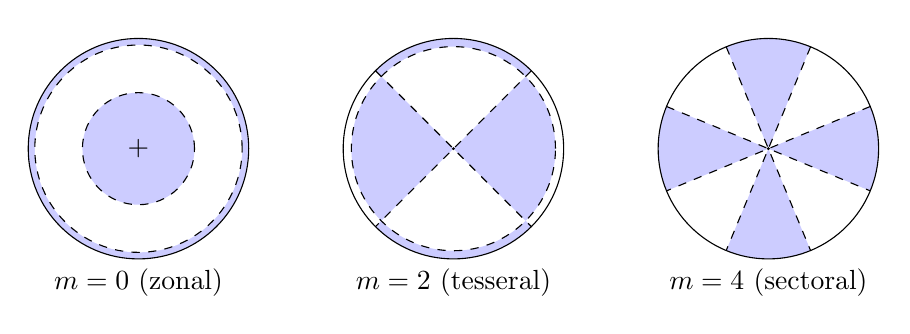
\begin{tikzpicture}
\begin{scope}
\fill[blue!20] (0,0) circle (1.4);
\fill[white] (0,0) circle ({1.4*sqrt(1-(15-2*sqrt(30))/35)});
\fill[blue!20] (0,0) circle ({1.4*sqrt(1-(15+2*sqrt(30))/35)});
\draw (0,0) circle (1.4);
\draw[dashed] (0,0) circle ({1.4*sqrt(1-(15-2*sqrt(30))/35)});
\draw[dashed] (0,0) circle ({1.4*sqrt(1-(15+2*sqrt(30))/35)});
\node at (0,0) {$+$};
\node at (0,-1.7) {$m=0$ (zonal)};
\end{scope}
\begin{scope}[xshift=4cm]
\foreach \s in {-45,135} {
\fill[blue!20] (0,0)--(\s:{1.4*sqrt(6/7)})
 arc[start angle=\s,end angle=\s+90,radius={1.4*sqrt(6/7)}]--cycle;}
\foreach \s in {45,225} {
\fill[blue!20] (\s:1.4)
 arc[start angle=\s,end angle=\s+90,radius=1.4]
 --(\s+90:{1.4*sqrt(6/7)})
 arc[start angle=\s+90,end angle=\s,radius={1.4*sqrt(6/7)}]--cycle;}
\draw (0,0) circle (1.4);
\draw[dashed] (0,0) circle ({1.4*sqrt(6/7)});
\draw[dashed] (45:1.4)--(225:1.4) (135:1.4)--(315:1.4);
\fill (0,0) circle (.02);
\node at (0,-1.7) {$m=2$ (tesseral)};
\end{scope}
\begin{scope}[xshift=8cm]
\foreach \s in {-22.5,67.5,157.5,247.5} {
\fill[blue!20] (0,0)--(\s:1.4)
 arc[start angle=\s,end angle=\s+45,radius=1.4]--cycle;}
\draw (0,0) circle (1.4);
\foreach \s in {22.5,67.5,112.5,157.5} {
\draw[dashed] (\s:1.4)--(\s+180:1.4);}
\fill (0,0) circle (.02);
\node at (0,-1.7) {$m=4$ (sectoral)};
\end{scope}
\end{tikzpicture}
\end{center}
For $m=0$, the latitude zeros solve $35y^2-30y+3=0$ with $y=x^2$, so
$x^2=(30\pm\sqrt{900-420})/70=(15\pm2\sqrt{30})/35$, that is,
$x\approx0.861$ and $0.340$ ($\theta\approx30.6^\circ$ and
$70.1^\circ$, $\rho\approx0.508$ and $0.940$). Since $P_4(1)=1>0$ and
$P_4(0)=3/8>0$, the polar cap and the equatorial band
are positive, and the band between them is negative.
For $m=2$, the factor $7x^2-1$ gives the latitude zero $x=1/\sqrt7$
($\rho=\sqrt{6/7}$), and the zeros of $\cos2\varphi$ give the
meridians $\varphi=\pi/4+j\pi/2$. Inside that latitude
circle ($x>1/\sqrt7$, where $7x^2-1>0$) the sign is that of
$\cos2\varphi$; outside it the sign reverses.
For $m=4$ there are no interior latitude zeros, and positivity is
$\cos4\varphi>0$, namely sectors centered at $\varphi=j\pi/2$
of half-width $\pi/8$. The pole is also a zero for $m=2,4$.
Since $n+m$ is even in all three cases, each function is even in $x$
($P_n^m(-x)=(-1)^{n+m}P_n^m(x)$, Exercise 15.5.1), so the southern
hemisphere has the same pattern.

\Needspace{5\baselineskip}
\par\bigskip
\noindent\textbf{15.5.7}\quad Suppose $f(r,\theta,\varphi)$ has the regular Laplace
series below, \erratum{converging uniformly on the closed ball
under consideration}:
\[
f(r,\theta,\varphi)=\sum_{l,m}a_{lm}r^{l}Y_{l}^{m}(\theta,\varphi).
\]
Letting $\langle\cdots\rangle_{\mathrm{sphere}}$ denote the average
over a sphere centered on the origin, show that
\[
\big\langle f(r,\theta,\varphi)\big\rangle_{\mathrm{sphere}}=f(0,0,0).
\]
\solution
Use $Y_0^0=1/\sqrt{4\pi}$ and orthogonality:
\[
\int Y_l^m\,d\Omega
=\sqrt{4\pi}\int Y_l^m(Y_0^0)^*d\Omega
=\sqrt{4\pi}\,\delta_{l0}\delta_{m0}.
\]
The average over the sphere of radius $r$ is
$\langle f\rangle_{\rm sphere}=(4\pi)^{-1}\int f(r,\theta,\varphi)\,d\Omega$.
Integrating the regular solid-harmonic expansion term by term, which the
assumed uniform convergence permits, therefore leaves only its constant
term:
\[
\langle f\rangle_{\rm sphere}
=\frac1{4\pi}\sum_{l,m}a_{lm}r^l\int Y_l^m\,d\Omega
=\frac{a_{00}}{\sqrt{4\pi}}.
\]
At the origin every $r^lY_l^m$ with $l>0$ vanishes, whereas
the $l=0$ term has the same value $a_{00}Y_0^0=a_{00}/\sqrt{4\pi}$.
Thus
\[
\boxed{\langle f\rangle_{\rm sphere}=f(0,0,0)}.
\]
\erratum{This is the mean-value property for the assumed regular
harmonic expansion. It does not hold for an arbitrary function;
for example, $f=r^2$ has sphere average $r^2$ but $f(0)=0$.}

\Needspace{8\baselineskip}
\subsection*{15.6 Legendre Functions of the Second Kind}

\Needspace{5\baselineskip}
\par\bigskip
\noindent\textbf{15.6.1}\quad \erratum{Use the real branches specified in the solution, with
$x\in\mathbb R\setminus\{-1,1\}$ and integer $l\ge0$.}
Show that if $l$ is even,
$Q_{l}(-x)=-Q_{l}(x)$, and that if $l$ is odd, $Q_{l}(-x)=Q_{l}(x)$.
\solution
Use the real Legendre functions with
\[
Q_0(x)=\frac12\ln\left|\frac{1+x}{1-x}\right|,\qquad
Q_1(x)=xQ_0(x)-1,\qquad x\ne\pm1.
\]
Replacing $x$ by $-x$ replaces the argument $|(1+x)/(1-x)|$ of the
logarithm by its reciprocal:
$Q_0(-x)=\frac12\ln|(1-x)/(1+x)|=-Q_0(x)$, so $Q_0$ is odd, and then
$Q_1(-x)=(-x)(-Q_0(x))-1=Q_1(x)$, so $Q_1$ is even. Thus
$Q_l(-x)=(-1)^{l+1}Q_l(x)$ holds for $l=0,1$.
The $Q_l$ obey the same three-term recurrence as the $P_l$,
$(n+1)Q_{n+1}(x)=(2n+1)xQ_n(x)-nQ_{n-1}(x)$.
Assume $Q_n(-x)=(-1)^{n+1}Q_n(x)$ and
$Q_{n-1}(-x)=(-1)^nQ_{n-1}(x)$ for some $n\ge1$. Then the
recurrence at $-x$ and $-(-1)^{n+1}=(-1)^{n+2}=(-1)^n$ give
\begin{align*}
(n+1)Q_{n+1}(-x)
&=-(2n+1)x(-1)^{n+1}Q_n(x)-n(-1)^nQ_{n-1}(x)\\
&=(-1)^{n+2}[(2n+1)xQ_n(x)-nQ_{n-1}(x)]\\
&=(-1)^{n+2}(n+1)Q_{n+1}(x).
\end{align*}
Induction proves
\[
\boxed{Q_l(-x)=(-1)^{l+1}Q_l(x)}.
\]
In particular even degree gives an odd function and odd degree an
even function. The assertion refers to these real functions (the
usual real $Q_l$ both for $|x|<1$ and for $|x|>1$); another choice of
branch of the logarithm would add a multiple of $P_l$, whose parity
$(-1)^l$ is the opposite one.

\Needspace{5\baselineskip}
\par\bigskip
\noindent\textbf{15.6.2}\quad Show that, \erratum{for nonnegative integers $p$ and
the real analytic $Q_l$ branch at $x=0$},
\begin{enumerate}
\item[(a)]
$\begin{aligned}[t]
Q_{2p}(x)=(-1)^{p}2^{2p}&\sum_{s=0}^{p}(-1)^{s}
\frac{(p+s)!\,(p-s)!}{(2s+1)!\,(2p-2s)!}\,x^{2s+1}\\
&+2^{2p}\sum_{s=p+1}^{\infty}
\frac{(p+s)!\,(2s-2p)!}{(2s+1)!\,(s-p)!}\,x^{2s+1},\qquad|x|<1,
\end{aligned}$
\item[(b)]
$\begin{aligned}[t]
Q_{2p+1}(x)=(-1)^{p+1}2^{2p}&\sum_{s=0}^{p}(-1)^{s}
\frac{(p+s)!\,(p-s)!}{(2s)!\,(2p-2s+1)!}\,x^{2s}\\
&+2^{2p+1}\sum_{s=p+1}^{\infty}
\frac{(p+s)!\,(2s-2p-2)!}{(2s)!\,(s-p-1)!}\,x^{2s},\qquad|x|<1.
\end{aligned}$
\end{enumerate}
\solution
Use the real analytic branch at $x=0$. As in Exercise 15.6.1, another
branch of the logarithm would add a multiple of $P_l$ (for example,
the exterior $Q_l$ continued onto $-1<x<1$ from above or below the
real axis equals this real function $\mp\frac{i\pi}2P_l(x)$), and
$P_l$ has only powers of the parity that is absent from the stated
series. Substituting
$y=\sum_ja_jx^j$ into $(1-x^2)y''-2xy'+l(l+1)y=0$, the coefficient of
$x^j$ is $(j+2)(j+1)a_{j+2}-j(j-1)a_j-2ja_j+l(l+1)a_j$, so the Legendre
equation gives the coefficient recurrence for any Taylor solution:
\[
(j+2)(j+1)a_{j+2}
=[j(j+1)-l(l+1)]a_j.
\]
By Exercise 15.6.1, $Q_{2p}$ is odd and $Q_{2p+1}$ is even, so their
Taylor series contain only odd and only even powers, respectively, and
the recurrence determines them from $Q'_{2p}(0)$ and $Q_{2p+1}(0)$.
These initial scales follow from $Q_0=x+\cdots$, $Q_1=-1+\cdots$
and the degree recurrences:
\[
Q'_{2p}(0)=(-1)^p\frac{(2p)!!}{(2p-1)!!},\qquad
Q_{2p+1}(0)=(-1)^{p+1}\frac{(2p)!!}{(2p+1)!!}.
\]
For the odd-degree values, the three-term recurrence
$(n+1)Q_{n+1}=(2n+1)xQ_n-nQ_{n-1}$ at $x=0$ with $n=2p$ gives
$(2p+1)Q_{2p+1}(0)=-2pQ_{2p-1}(0)$; iterating down to $Q_1(0)=-1$,
\[
Q_{2p+1}(0)=\prod_{k=1}^p\left(-\frac{2k}{2k+1}\right)Q_1(0)
=(-1)^{p+1}\frac{(2p)!!}{(2p+1)!!}.
\]
For the even-degree derivative, the identity
$(1-x^2)Q'_n=n(Q_{n-1}-xQ_n)$, which the $Q_n$ share with the $P_n$,
gives with $n=2p$ at $x=0$, and the odd-degree value for
$2p-1=2(p-1)+1$,
\[
Q'_{2p}(0)=2pQ_{2p-1}(0)
=(-1)^p\frac{2p(2p-2)!!}{(2p-1)!!}
=(-1)^p\frac{(2p)!!}{(2p-1)!!}\quad(p\ge1).
\]
The case $p=0$ comes from $Q_0$. With $(2p)!!=2^pp!$,
$(2p-1)!!=(2p)!/(2^pp!)$ and $(2p+1)!!=(2p+1)!/(2^pp!)$, these are
the values $C_0$ and $D_0$ below.

(a) Write $Q_{2p}=\sum_{s\ge0}C_sx^{2s+1}$.
For $j=2s+1$ and $l=2p$,
$(2s+1)(2s+2)-2p(2p+1)=2(s+p+1)(2s-2p+1)$, so
the Taylor recurrence is
\[
\frac{C_{s+1}}{C_s}
=\frac{(s+p+1)(2s-2p+1)}{(s+1)(2s+3)},\qquad
C_0=(-1)^p2^{2p}\frac{(p!)^2}{(2p)!}.
\]
For $0\le s\le p$, its product gives
\[
C_s=(-1)^{p+s}2^{2p}
\frac{(p+s)!(p-s)!}{(2s+1)!(2p-2s)!},
\]
which equals $C_0$ at $s=0$.
To check the product explicitly, the factorial ratio between adjacent
terms of this formula ($0\le s\le p-1$) is, with $(2p-2s)/(p-s)=2$,
\[
-\frac{p+s+1}{p-s}
\frac{(2p-2s)(2p-2s-1)}{(2s+3)(2s+2)}
=\frac{(p+s+1)(2s-2p+1)}{(s+1)(2s+3)}.
\]
At the transition, the formula gives $C_p=2^{2p}/(2p+1)$, and the
recurrence with $s=p$ gives
$C_{p+1}=C_p(2p+1)/[(p+1)(2p+3)]=2^{2p}/[(p+1)(2p+3)]$.
For $s\ge p+1$, the all-positive continuation is
\[
C_s=2^{2p}\frac{(p+s)!(2s-2p)!}{(2s+1)!(s-p)!},
\]
which reproduces $C_{p+1}$ at $s=p+1$. Its adjacent ratio,
\[
\frac{(p+s+1)(2s-2p+2)(2s-2p+1)}{(2s+3)(2s+2)(s-p+1)},
\]
reduces to the same recurrence by canceling
$2s-2p+2=2(s-p+1)$ against $s-p+1$. These formulas give exactly the two
sums in part (a).

(b) Put $Q_{2p+1}=\sum_{s\ge0}D_sx^{2s}$. This time $j=2s$,
$l=2p+1$, and
$2s(2s+1)-(2p+1)(2p+2)=2(s+p+1)(2s-2p-1)$, so
\[
\frac{D_{s+1}}{D_s}
=\frac{(s+p+1)(2s-2p-1)}{(s+1)(2s+1)},\qquad
D_0=(-1)^{p+1}2^{2p}\frac{(p!)^2}{(2p+1)!}.
\]
For $0\le s\le p$, repeated multiplication gives
\[
D_s=(-1)^{p+1+s}2^{2p}
\frac{(p+s)!(p-s)!}{(2s)!(2p-2s+1)!},
\]
which equals $D_0$ at $s=0$.
Its ratio ($0\le s\le p-1$) is
$-(p+s+1)(2p-2s+1)(2p-2s)/
[(p-s)(2s+2)(2s+1)]$, equal to the required ratio after canceling
$(2p-2s)/(p-s)=2$ against $2s+2=2(s+1)$ and writing
$-(2p-2s+1)=2s-2p-1$.
At the transition, the formula gives $D_p=-2^{2p}$, and the recurrence
with $s=p$ gives $D_{p+1}=D_p(2p+1)(-1)/[(p+1)(2p+1)]=2^{2p}/(p+1)$.
For the positive tail,
\[
D_s=2^{2p+1}\frac{(p+s)!(2s-2p-2)!}{(2s)!(s-p-1)!},
\qquad s\ge p+1,
\]
which reproduces $D_{p+1}=2^{2p+1}/(2p+2)$ at $s=p+1$. Its adjacent
ratio is
$(p+s+1)(2s-2p)(2s-2p-1)/[(2s+2)(2s+1)(s-p)]$, and canceling
$2s-2p=2(s-p)$ against $s-p$ again gives the same recurrence.
The initial values, the ratios within each range and the transition
values therefore establish both requested sums for every $s\ge0$.
Their term ratios tend to $x^2$, proving convergence
for $|x|<1$; uniqueness of the Taylor solution identifies them with $Q_l$.

\Needspace{5\baselineskip}
\par\bigskip
\noindent\textbf{15.6.3}
\begin{enumerate}
\item[(a)] \erratum{Use integer $l\ge0$ and the exterior $Q_l$
branch decaying at infinity, on $|x|>1$.} Starting with the assumed form
\[
Q_{l}(x)=\sum_{j=0}^{\infty}b_{lj}x^{k-j},
\]
show that
\[
Q_{l}(x)=b_{l0}x^{-l-1}\sum_{s=0}^{\infty}
\frac{(l+s)!\,(l+2s)!\,(2l+1)!}{s!\,(l!)^{2}(2l+2s+1)!}\,x^{-2s}.
\]
\item[(b)] The standard choice of $b_{l0}$ is
\[
b_{l0}=\frac{2^{l}(l!)^{2}}{(2l+1)!},
\]
leading to the final result
\[
Q_{l}(x)=x^{-l-1}\sum_{s=0}^{\infty}
\frac{(l+2s)!}{(2s)!!\,(2l+2s+1)!!}\,x^{-2s}.
\]
Show that this choice of $b_{l0}$ brings this negative power-series
form of $Q_{n}(x)$ into agreement with the closed-form solutions.
\end{enumerate}
\solution
(a) For a monomial $x^\alpha$, the Legendre operator
$L_l=(1-x^2)\,d^2/dx^2-2x\,d/dx+l(l+1)$ gives
$(1-x^2)\alpha(\alpha-1)x^{\alpha-2}-2\alpha x^\alpha+l(l+1)x^\alpha$,
that is,
\[
L_l[x^\alpha]=\alpha(\alpha-1)x^{\alpha-2}
+[l(l+1)-\alpha(\alpha+1)]x^\alpha.
\]
The leading term $b_{l0}x^k$ ($b_{l0}\ne0$) of the proposed series
gives the highest power $x^k$, with coefficient
$[l(l+1)-k(k+1)]b_{l0}$; the equation therefore requires
$k(k+1)=l(l+1)$, giving $k=l$ or $k=-l-1$.
The solution that decays at infinity uses the latter root.
The power $x^{k-j}=x^{-l-1-j}$ then receives
$[l(l+1)-(l+j)(l+j+1)]b_{lj}=-j(2l+j+1)b_{lj}$ from the term $j$, and,
through $\alpha(\alpha-1)x^{\alpha-2}$ with $\alpha=-l-j+1$,
$(l+j-1)(l+j)b_{l,j-2}$ from the term $j-2$. Hence
\[
j(2l+j+1)b_{lj}=(l+j)(l+j-1)b_{l,j-2},\qquad b_{l,-1}=0.
\]
At $j=1$, the power $x^{-l-2}$, this says
$2(l+1)b_{l1}=0$.
It follows that $b_{l1}=0$, and the recurrence then makes every
odd $j$ vanish. Set $c_s=b_{l,2s}$.
At power $x^{-l-1-2s}$ ($j=2s$) the equation gives
\[
2s(2l+2s+1)c_s=(l+2s)(l+2s-1)c_{s-1}.
\]
Hence
\[
\frac{c_s}{c_0}
=\prod_{q=1}^s\frac{(l+2q)(l+2q-1)}{2q(2l+2q+1)}
=\frac{(l+s)!(l+2s)!(2l+1)!}
{s!(l!)^2(2l+2s+1)!}.
\]
For the last equality, the numerator product is
$(l+1)(l+2)\cdots(l+2s)=(l+2s)!/l!$,
while the denominator product is
$2^ss!\,(2l+3)(2l+5)\cdots(2l+2s+1)=2^ss!\,(2l+2s+1)!!/(2l+1)!!$;
with $(2N+1)!!=(2N+1)!/(2^NN!)$ for $N=l+s$ and $N=l$, this is
$s!\,l!(2l+2s+1)!/[(l+s)!(2l+1)!]$.
This proves the requested series. Since
$c_s/c_{s-1}=(l+2s)(l+2s-1)/[2s(2l+2s+1)]\to1$, the ratio of
successive terms tends to $x^{-2}$, and the series converges for
$|x|>1$.

(b) The normalization can be checked against the closed logarithmic
solutions for every degree by the integral
\[
R_l(z)=\frac12\int_{-1}^1\frac{P_l(t)}{z-t}dt,\qquad |z|>1.
\]
Directly, since $-\operatorname{Log}(z-t)$ is an antiderivative of
$1/(z-t)$,
$R_0=\tfrac12[\operatorname{Log}(z+1)-\operatorname{Log}(z-1)]
=\tfrac12\operatorname{Log}[(z+1)/(z-1)]$ with the branch
vanishing at infinity (for real $z>1$ this is
$\frac12\ln[(z+1)/(z-1)]=Q_0(z)$), and, with $t/(z-t)=z/(z-t)-1$,
$R_1=\frac12\int_{-1}^1[z/(z-t)-1]dt=zR_0-1=Q_1(z)$.
For $l\ge1$, multiply the polynomial degree recurrence
$(l+1)P_{l+1}(t)=(2l+1)tP_l(t)-lP_{l-1}(t)$ by
$1/[2(z-t)]$, integrate over $[-1,1]$, and use
$t/(z-t)=z/(z-t)-1$ and $\int_{-1}^1P_l\,dt=0$; the middle term
becomes $(2l+1)[zR_l-\frac12\int_{-1}^1P_l\,dt]=(2l+1)zR_l$. This gives
\[
(l+1)R_{l+1}=(2l+1)zR_l-lR_{l-1}.
\]
The closed forms $Q_l$ obey the same recurrence and have the same
first two members, so $R_l=Q_l$ for every $l$ by induction.
For $|t|\le1<|z|$ the geometric series
$1/(z-t)=\sum_{j\ge0}t^jz^{-j-1}$ converges uniformly in $t$, so it may
be integrated term by term under the finite integral:
$R_l(z)=\sum_{j\ge0}z^{-j-1}\,\frac12\int_{-1}^1t^jP_l(t)dt$.
All moments with $j<l$ vanish by orthogonality ($t^j$ is a combination
of $P_0,\ldots,P_j$), so the series starts with $z^{-l-1}$, as in part
(a), and its leading coefficient is the moment with $j=l$. Since $P_l$
has leading coefficient $(2l)!/[2^l(l!)^2]$, $t^l$ equals
$2^l(l!)^2P_l(t)/(2l)!$ plus a polynomial of lower degree; with
$\int_{-1}^1P_l^2dt=2/(2l+1)$,
\[
b_{l0}=\frac12\int_{-1}^1t^lP_l(t)dt
=\frac{2^l(l!)^2}{(2l)!}\,\frac1{2l+1}
=\boxed{\frac{2^l(l!)^2}{(2l+1)!}}.
\]
Because $R_l=Q_l$ satisfies Legendre's equation and, for $|z|>1$,
equals this convergent series in descending powers beginning with
$z^{-l-1}$ (the form assumed in part (a), with $k=-l-1$), the
recurrence of part (a) applies to its coefficients; they are therefore
$b_{l0}$ times the coefficients found there:
\[
b_{l0}\frac{(l+s)!(l+2s)!(2l+1)!}{s!(l!)^2(2l+2s+1)!}
=\frac{2^l(l+s)!(l+2s)!}{s!(2l+2s+1)!},
\]
and splitting even and odd factorials,
$(2l+2s+1)!=2^{l+s}(l+s)!\,(2l+2s+1)!!$ and $2^ss!=(2s)!!$, gives
\[
\boxed{Q_l(z)=z^{-l-1}\sum_{s=0}^\infty
\frac{(l+2s)!}{(2s)!!(2l+2s+1)!!}z^{-2s}},\qquad |z|>1.
\]
For example, for $l=0$ the coefficients are
$(2s)!/[(2s)!!(2s+1)!!]=(2s)!/(2s+1)!=1/(2s+1)$, and
$\sum_sz^{-2s-1}/(2s+1)=\frac12\ln[(z+1)/(z-1)]$ is the familiar
expansion of $Q_0$.
For complex $z$ with $|z|>1$ the integral $R_l$ and the series define
the same branch of $Q_l$, the one that is analytic outside $[-1,1]$ and
vanishes at infinity.

\Needspace{5\baselineskip}
\par\bigskip
\noindent\textbf{15.6.4}
\begin{enumerate}
\item[(a)] Using the recurrence relations, prove (independent of the
Wronskian relation) that, \erratum{for integers $n\ge1$ on a common
consistent branch away from $x=\pm1$},
\[
n\big[P_{n}(x)Q_{n-1}(x)-P_{n-1}(x)Q_{n}(x)\big]
=P_{1}(x)Q_{0}(x)-P_{0}(x)Q_{1}(x).
\]
\item[(b)] By direct substitution show that the right-hand side of
this equation equals 1.
\end{enumerate}
\solution
(a) Let $D_n=P_nQ_{n-1}-P_{n-1}Q_n$. For $n\ge2$, both families obey
the three-term recurrence (with $n$ shifted to $n-1$)
\[
nF_n=(2n-1)xF_{n-1}-(n-1)F_{n-2}.
\]
Substitute this for $nP_n$ and $nQ_n$ in $nD_n=(nP_n)Q_{n-1}-P_{n-1}(nQ_n)$;
the terms $\pm(2n-1)xP_{n-1}Q_{n-1}$ cancel:
\begin{align*}
nD_n
&=[(2n-1)xP_{n-1}-(n-1)P_{n-2}]Q_{n-1}\\
&\quad-P_{n-1}[(2n-1)xQ_{n-1}-(n-1)Q_{n-2}]\\
&=(n-1)[P_{n-1}Q_{n-2}-P_{n-2}Q_{n-1}]\\
&=(n-1)D_{n-1}.
\end{align*}
Repeating gives $nD_n=(n-1)D_{n-1}=(n-2)D_{n-2}=\cdots=1\cdot D_1$,
which is the stated identity, since $D_1=P_1Q_0-P_0Q_1$; the case
$n=1$ is trivially included.

(b) Finally $P_0=1$, $P_1=x$, and $Q_1=xQ_0-1$, so
\[
D_1=xQ_0-(xQ_0-1)=1.
\]
Therefore
\[
\boxed{n[P_nQ_{n-1}-P_{n-1}Q_n]=1}.
\]
The argument uses only degree recurrences and starting values, as
requested, and is valid on any common consistent branch away from
the singular endpoints.
